% generated from JIRA project LVV
% using template at /usr/share/miniconda/envs/docsteady-env/lib/python3.12/site-packages/docsteady/templates/tpr.latex.jinja2.
% using docsteady version 0.0.0
% Please do not edit -- update information in Jira instead
\documentclass[DM,lsstdraft,STR,toc]{lsstdoc}
\usepackage{geometry}
\usepackage{longtable,booktabs}
\usepackage{enumitem}
\usepackage{arydshln}
\usepackage{attachfile}
\usepackage{array}
\usepackage{dashrule}
\usepackage{pdfpages}

\newcolumntype{L}[1]{>{\raggedright\let\newline\\\arraybackslash\hspace{0pt}}p{#1}}

\input{meta.tex}

\newcommand{\attachmentsUrl}{https://github.com/\gitorg/\lsstDocType-\lsstDocNum/blob/\gitref/attachments}
\providecommand{\tightlist}{
  \setlength{\itemsep}{0pt}\setlength{\parskip}{0pt}}

\setcounter{tocdepth}{4}

\providecommand{\ul}[1]{\textbf{#1}}

\begin{document}

\def\milestoneName{Data Management Acceptance Test Campaign, Fall 2023}
\def\milestoneId{}
\def\product{Acceptance}

\setDocCompact{true}

\title{LVV-P106: Data Management Acceptance Test Campaign, Fall 2023 Test Plan and Report}
\setDocRef{\lsstDocType-\lsstDocNum}
\date{ 2023-10-20 }
\author{ Jeffrey Carlin }

% Most recent last
\setDocChangeRecord{
\addtohist{}{2023-07-01}{First draft}{Jeffrey Carlin}
\addtohist{}{2024-04-08}{Test campaign LVV-P106 completed and results approved. DM-40311}{Jeffrey Carlin}
}

\setDocCurator{Jeffrey Carlin}
\setDocUpstreamLocation{\url{https://github.com/lsst-dm/\lsstDocType-\lsstDocNum}}
\setDocUpstreamVersion{\vcsRevision}



\setDocAbstract{
This is the test plan and report for
\textbf{ Data Management Acceptance Test Campaign, Fall 2023},
an LSST milestone pertaining to the Data Management Subsystem.\\
This document is based on content automatically extracted from the Jira test database on \docDate.
The most recent change to the document repository was on \vcsDate.
}


\maketitle

\section{Introduction}
\label{sect:intro}


\subsection{Objectives}
\label{sect:objectives}

 The primary goal of this DM acceptance test campaign will be to verify
priority 1a DMSR (\citeds{LSE-61}) requirements that have not been verified as
part of prior testing and milestones. Any priority 1b, 2, or 3
requirements that have been completed will also be verified.



\subsection{System Overview}
\label{sect:systemoverview}

 This test campaign is intended to verify that the DM system satisfies at
least half of the priority 1a requirements outlined in the Data
Management System Requirements (DMSR;
\href{https://lse-61.lsst.io/}{LSE-61} ), ensuring that we are
progressing toward readiness for the installation and operation of
LSSTCam. Additional DMSR requirements will be verified in later
Acceptance Test Campaigns.\\
\strut \\
\textbf{Applicable Documents:}\\
\citeds{LSE-61}: Data Management System (DMS) Requirements\\
\citeds{LDM-503} Data Management Test Plan\\
\citeds{LDM-639}: Data Management Acceptance Test Specification\\
\strut \\
Tests in this campaign will use data products and artifacts from Data
Preview 0.2, which consists of DESC Data Challenge 2 (DC2) simulated
data reprocessed using the LSST Science Pipelines. Additional on-sky
data from auxTel imaging campaigns, and camera test-stand data, will be
used when appropriate.


\subsection{Document Overview}
\label{sect:docoverview}

This document was generated from Jira, obtaining the relevant information from the
\href{https://jira.lsstcorp.org/secure/Tests.jspa\#/testPlan/LVV-P106}{LVV-P106}
~Jira Test Plan and related Test Cycles (
\href{https://jira.lsstcorp.org/secure/Tests.jspa\#/testCycle/LVV-C260}{LVV-C260}
).

Section \ref{sect:intro} provides an overview of the test campaign, the system under test (\product{}),
the applicable documentation, and explains how this document is organized.
Section \ref{sect:testplan} provides additional information about the test plan, like for example the configuration
used for this test or related documentation.
Section \ref{sect:personnel} describes the necessary roles and lists the individuals assigned to them.

Section \ref{sect:overview} provides a summary of the test results, including an overview in Table \ref{table:summary},
an overall assessment statement and suggestions for possible improvements.
Section \ref{sect:detailedtestresults} provides detailed results for each step in each test case.

The current status of test plan \href{https://jira.lsstcorp.org/secure/Tests.jspa\#/testPlan/LVV-P106}{LVV-P106} in Jira is \textbf{ Approved }.

\subsection{References}
\label{sect:references}
\renewcommand{\refname}{}
\bibliography{lsst,refs,books,refs_ads,local}


\newpage
\section{Test Plan Details}
\label{sect:testplan}


\subsection{Data Collection}

  Observing is not required for this test campaign.

\subsection{Verification Environment}
\label{sect:hwconf}
  Most testing will be performed using the Rubin Science Platform (RSP)
and the development cluster at the USDF. In particular, we will use
version 26 of the Pipelines for most tests; some tests will use more
recent weekly builds of the Pipelines.




\subsection{Related Documentation}


No additional documentation provided.


\subsection{PMCS Activity}

Primavera milestones related to the test campaign:
\begin{itemize}
\item None
\end{itemize}


\newpage
\section{Personnel}
\label{sect:personnel}

The personnel involved in the test campaign is shown in the following table.

{\small
\begin{longtable}{p{3cm}p{3cm}p{3cm}p{6cm}}
\hline
\multicolumn{2}{r}{T. Plan \href{https://jira.lsstcorp.org/secure/Tests.jspa\#/testPlan/LVV-P106}{LVV-P106} owner:} &
\multicolumn{2}{l}{\textbf{ Jeffrey Carlin } }\\\hline
\multicolumn{2}{r}{T. Cycle \href{https://jira.lsstcorp.org/secure/Tests.jspa\#/testCycle/LVV-C260}{LVV-C260} owner:} &
\multicolumn{2}{l}{\textbf{
Jeffrey Carlin }
} \\\hline
\textbf{Test Cases} & \textbf{Assigned to} & \textbf{Executed by} & \textbf{Additional Test Personnel} \\ \hline
\href{https://jira.lsstcorp.org/secure/Tests.jspa#/testCase/LVV-T1240}{LVV-T1240}
& {\small Jim Bosch } & {\small Jeffrey Carlin } &
\begin{minipage}[]{6cm}
\smallskip
{\small  }
\medskip
\end{minipage}
\\ \hline
\href{https://jira.lsstcorp.org/secure/Tests.jspa#/testCase/LVV-T191}{LVV-T191}
& {\small Leanne Guy } & {\small  } &
\begin{minipage}[]{6cm}
\smallskip
{\small  }
\medskip
\end{minipage}
\\ \hline
\href{https://jira.lsstcorp.org/secure/Tests.jspa#/testCase/LVV-T1986}{LVV-T1986}
& {\small Leanne Guy } & {\small  } &
\begin{minipage}[]{6cm}
\smallskip
{\small  }
\medskip
\end{minipage}
\\ \hline
\href{https://jira.lsstcorp.org/secure/Tests.jspa#/testCase/LVV-T159}{LVV-T159}
& {\small Leanne Guy } & {\small  } &
\begin{minipage}[]{6cm}
\smallskip
{\small  }
\medskip
\end{minipage}
\\ \hline
\href{https://jira.lsstcorp.org/secure/Tests.jspa#/testCase/LVV-T132}{LVV-T132}
& {\small Leanne Guy } & {\small  } &
\begin{minipage}[]{6cm}
\smallskip
{\small  }
\medskip
\end{minipage}
\\ \hline
\href{https://jira.lsstcorp.org/secure/Tests.jspa#/testCase/LVV-T62}{LVV-T62}
& {\small Jim Bosch } & {\small Jeffrey Carlin } &
\begin{minipage}[]{6cm}
\smallskip
{\small  }
\medskip
\end{minipage}
\\ \hline
\href{https://jira.lsstcorp.org/secure/Tests.jspa#/testCase/LVV-T168}{LVV-T168}
& {\small Leanne Guy } & {\small  } &
\begin{minipage}[]{6cm}
\smallskip
{\small  }
\medskip
\end{minipage}
\\ \hline
\href{https://jira.lsstcorp.org/secure/Tests.jspa#/testCase/LVV-T41}{LVV-T41}
& {\small Jim Bosch } & {\small Jeffrey Carlin } &
\begin{minipage}[]{6cm}
\smallskip
{\small  }
\medskip
\end{minipage}
\\ \hline
\href{https://jira.lsstcorp.org/secure/Tests.jspa#/testCase/LVV-T97}{LVV-T97}
& {\small Kian-Tat Lim } & {\small  } &
\begin{minipage}[]{6cm}
\smallskip
{\small  }
\medskip
\end{minipage}
\\ \hline
\href{https://jira.lsstcorp.org/secure/Tests.jspa#/testCase/LVV-T2177}{LVV-T2177}
& {\small Leanne Guy } & {\small  } &
\begin{minipage}[]{6cm}
\smallskip
{\small  }
\medskip
\end{minipage}
\\ \hline
\href{https://jira.lsstcorp.org/secure/Tests.jspa#/testCase/LVV-T1755}{LVV-T1755}
& {\small Jeffrey Carlin } & {\small  } &
\begin{minipage}[]{6cm}
\smallskip
{\small  }
\medskip
\end{minipage}
\\ \hline
\href{https://jira.lsstcorp.org/secure/Tests.jspa#/testCase/LVV-T2176}{LVV-T2176}
& {\small Leanne Guy } & {\small  } &
\begin{minipage}[]{6cm}
\smallskip
{\small  }
\medskip
\end{minipage}
\\ \hline
\href{https://jira.lsstcorp.org/secure/Tests.jspa#/testCase/LVV-T1754}{LVV-T1754}
& {\small Jeffrey Carlin } & {\small  } &
\begin{minipage}[]{6cm}
\smallskip
{\small  }
\medskip
\end{minipage}
\\ \hline
\href{https://jira.lsstcorp.org/secure/Tests.jspa#/testCase/LVV-T376}{LVV-T376}
& {\small Leanne Guy } & {\small  } &
\begin{minipage}[]{6cm}
\smallskip
{\small  }
\medskip
\end{minipage}
\\ \hline
\href{https://jira.lsstcorp.org/secure/Tests.jspa#/testCase/LVV-T1946}{LVV-T1946}
& {\small Jeffrey Carlin } & {\small  } &
\begin{minipage}[]{6cm}
\smallskip
{\small  }
\medskip
\end{minipage}
\\ \hline
\href{https://jira.lsstcorp.org/secure/Tests.jspa#/testCase/LVV-T1947}{LVV-T1947}
& {\small Jeffrey Carlin } & {\small  } &
\begin{minipage}[]{6cm}
\smallskip
{\small  }
\medskip
\end{minipage}
\\ \hline
\href{https://jira.lsstcorp.org/secure/Tests.jspa#/testCase/LVV-T28}{LVV-T28}
& {\small Colin Slater } & {\small  } &
\begin{minipage}[]{6cm}
\smallskip
{\small  }
\medskip
\end{minipage}
\\ \hline
\href{https://jira.lsstcorp.org/secure/Tests.jspa#/testCase/LVV-T124}{LVV-T124}
& {\small Jeffrey Carlin } & {\small  } &
\begin{minipage}[]{6cm}
\smallskip
{\small  }
\medskip
\end{minipage}
\\ \hline
\href{https://jira.lsstcorp.org/secure/Tests.jspa#/testCase/LVV-T142}{LVV-T142}
& {\small Colin Slater } & {\small  } &
\begin{minipage}[]{6cm}
\smallskip
{\small  }
\medskip
\end{minipage}
\\ \hline
\href{https://jira.lsstcorp.org/secure/Tests.jspa#/testCase/LVV-T1748}{LVV-T1748}
& {\small Jeffrey Carlin } & {\small  } &
\begin{minipage}[]{6cm}
\smallskip
{\small  }
\medskip
\end{minipage}
\\ \hline
\href{https://jira.lsstcorp.org/secure/Tests.jspa#/testCase/LVV-T1759}{LVV-T1759}
& {\small Jeffrey Carlin } & {\small Jeffrey Carlin } &
\begin{minipage}[]{6cm}
\smallskip
{\small  }
\medskip
\end{minipage}
\\ \hline
\href{https://jira.lsstcorp.org/secure/Tests.jspa#/testCase/LVV-T1758}{LVV-T1758}
& {\small Jeffrey Carlin } & {\small Jeffrey Carlin } &
\begin{minipage}[]{6cm}
\smallskip
{\small  }
\medskip
\end{minipage}
\\ \hline
\href{https://jira.lsstcorp.org/secure/Tests.jspa#/testCase/LVV-T149}{LVV-T149}
& {\small Leanne Guy } & {\small Jeffrey Carlin } &
\begin{minipage}[]{6cm}
\smallskip
{\small  }
\medskip
\end{minipage}
\\ \hline
\href{https://jira.lsstcorp.org/secure/Tests.jspa#/testCase/LVV-T40}{LVV-T40}
& {\small Jeffrey Carlin } & {\small Jeffrey Carlin } &
\begin{minipage}[]{6cm}
\smallskip
{\small  }
\medskip
\end{minipage}
\\ \hline
\href{https://jira.lsstcorp.org/secure/Tests.jspa#/testCase/LVV-T129}{LVV-T129}
& {\small Jeffrey Carlin } & {\small  } &
\begin{minipage}[]{6cm}
\smallskip
{\small  }
\medskip
\end{minipage}
\\ \hline
\href{https://jira.lsstcorp.org/secure/Tests.jspa#/testCase/LVV-T115}{LVV-T115}
& {\small Kian-Tat Lim } & {\small  } &
\begin{minipage}[]{6cm}
\smallskip
{\small  }
\medskip
\end{minipage}
\\ \hline
\href{https://jira.lsstcorp.org/secure/Tests.jspa#/testCase/LVV-T1862}{LVV-T1862}
& {\small Jeffrey Carlin } & {\small  } &
\begin{minipage}[]{6cm}
\smallskip
{\small  }
\medskip
\end{minipage}
\\ \hline
\href{https://jira.lsstcorp.org/secure/Tests.jspa#/testCase/LVV-T89}{LVV-T89}
& {\small Eli Rykoff } & {\small  } &
\begin{minipage}[]{6cm}
\smallskip
{\small  }
\medskip
\end{minipage}
\\ \hline
\href{https://jira.lsstcorp.org/secure/Tests.jspa#/testCase/LVV-T88}{LVV-T88}
& {\small Eli Rykoff } & {\small  } &
\begin{minipage}[]{6cm}
\smallskip
{\small  }
\medskip
\end{minipage}
\\ \hline
\href{https://jira.lsstcorp.org/secure/Tests.jspa#/testCase/LVV-T85}{LVV-T85}
& {\small Jeffrey Carlin } & {\small  } &
\begin{minipage}[]{6cm}
\smallskip
{\small  }
\medskip
\end{minipage}
\\ \hline
\href{https://jira.lsstcorp.org/secure/Tests.jspa#/testCase/LVV-T83}{LVV-T83}
& {\small Jeffrey Carlin } & {\small  } &
\begin{minipage}[]{6cm}
\smallskip
{\small  }
\medskip
\end{minipage}
\\ \hline
\end{longtable}
}

\newpage

\section{Test Campaign Overview}
\label{sect:overview}

\subsection{Summary}
\label{sect:summarytable}

{\small
\begin{longtable}{p{2cm}cp{2.3cm}p{8.6cm}p{2.3cm}}
\toprule
\multicolumn{2}{r}{ T. Plan \href{https://jira.lsstcorp.org/secure/Tests.jspa\#/testPlan/LVV-P106}{LVV-P106}:} &
\multicolumn{2}{p{10.9cm}}{\textbf{ Data Management Acceptance Test Campaign, Fall 2023 }} & Approved \\\hline
\multicolumn{2}{r}{ T. Cycle \href{https://jira.lsstcorp.org/secure/Tests.jspa\#/testCycle/LVV-C260}{LVV-C260}:} &
\multicolumn{2}{p{10.9cm}}{\textbf{ Data Management Acceptance Test Campaign, Fall 2023 }} & In Progress \\\hline
\textbf{Test Cases} &  \textbf{Ver.} & \textbf{Status} & \textbf{Comment} & \textbf{Issues} \\\toprule
\href{https://jira.lsstcorp.org/secure/Tests.jspa#/testCase/LVV-T1240}{LVV-T1240}
&  1
& Pass &
\begin{minipage}[]{9cm}
\smallskip
Test executed with science pipelines version w\_2023\_37 in the RSP
Notebook aspect at the USDF.\\
\strut \\
The executed notebook was saved in the repository associated with this
campaign's test report as ``notebooks/test\_LVV-T40\_T1240.ipynb''.
\medskip
\end{minipage}
&   \\\hline
\href{https://jira.lsstcorp.org/secure/Tests.jspa#/testCase/LVV-T191}{LVV-T191}
&  1
& Not Executed &
\begin{minipage}[]{9cm}
\smallskip

\medskip
\end{minipage}
&   \\\hline
\href{https://jira.lsstcorp.org/secure/Tests.jspa#/testCase/LVV-T1986}{LVV-T1986}
&  1
& Not Executed &
\begin{minipage}[]{9cm}
\smallskip

\medskip
\end{minipage}
&   \\\hline
\href{https://jira.lsstcorp.org/secure/Tests.jspa#/testCase/LVV-T159}{LVV-T159}
&  1
& Not Executed &
\begin{minipage}[]{9cm}
\smallskip

\medskip
\end{minipage}
&   \\\hline
\href{https://jira.lsstcorp.org/secure/Tests.jspa#/testCase/LVV-T132}{LVV-T132}
&  1
& Not Executed &
\begin{minipage}[]{9cm}
\smallskip

\medskip
\end{minipage}
&   \\\hline
\href{https://jira.lsstcorp.org/secure/Tests.jspa#/testCase/LVV-T62}{LVV-T62}
&  2
& Pass &
\begin{minipage}[]{9cm}
\smallskip
Test executed with science pipelines version w\_2023\_34 in the RSP
Notebook aspect at the USDF.\\
\strut \\
The executed notebook was saved in the repository associated with this
campaign's test report as ``notebooks/test\_LVV-T62.ipynb''.
\medskip
\end{minipage}
&   \\\hline
\href{https://jira.lsstcorp.org/secure/Tests.jspa#/testCase/LVV-T168}{LVV-T168}
&  1
& Not Executed &
\begin{minipage}[]{9cm}
\smallskip

\medskip
\end{minipage}
&   \\\hline
\href{https://jira.lsstcorp.org/secure/Tests.jspa#/testCase/LVV-T41}{LVV-T41}
&  1
& Pass &
\begin{minipage}[]{9cm}
\smallskip
Test executed with science pipelines version w\_2023\_37 in the RSP
Notebook aspect at the USDF.\\
\strut \\
The executed notebook was saved in the repository associated with this
campaign's test report as ``notebooks/test\_LVV-T41.ipynb''.
\medskip
\end{minipage}
&   \\\hline
\href{https://jira.lsstcorp.org/secure/Tests.jspa#/testCase/LVV-T97}{LVV-T97}
&  1
& Not Executed &
\begin{minipage}[]{9cm}
\smallskip

\medskip
\end{minipage}
&   \\\hline
\href{https://jira.lsstcorp.org/secure/Tests.jspa#/testCase/LVV-T2177}{LVV-T2177}
&  1
& Not Executed &
\begin{minipage}[]{9cm}
\smallskip

\medskip
\end{minipage}
&   \\\hline
\href{https://jira.lsstcorp.org/secure/Tests.jspa#/testCase/LVV-T1755}{LVV-T1755}
&  1
& Not Executed &
\begin{minipage}[]{9cm}
\smallskip

\medskip
\end{minipage}
&   \\\hline
\href{https://jira.lsstcorp.org/secure/Tests.jspa#/testCase/LVV-T2176}{LVV-T2176}
&  1
& Not Executed &
\begin{minipage}[]{9cm}
\smallskip

\medskip
\end{minipage}
&   \\\hline
\href{https://jira.lsstcorp.org/secure/Tests.jspa#/testCase/LVV-T1754}{LVV-T1754}
&  1
& Not Executed &
\begin{minipage}[]{9cm}
\smallskip

\medskip
\end{minipage}
&   \\\hline
\href{https://jira.lsstcorp.org/secure/Tests.jspa#/testCase/LVV-T376}{LVV-T376}
&  1
& Not Executed &
\begin{minipage}[]{9cm}
\smallskip

\medskip
\end{minipage}
&   \\\hline
\href{https://jira.lsstcorp.org/secure/Tests.jspa#/testCase/LVV-T1946}{LVV-T1946}
&  1
& Not Executed &
\begin{minipage}[]{9cm}
\smallskip

\medskip
\end{minipage}
&   \\\hline
\href{https://jira.lsstcorp.org/secure/Tests.jspa#/testCase/LVV-T1947}{LVV-T1947}
&  1
& Not Executed &
\begin{minipage}[]{9cm}
\smallskip

\medskip
\end{minipage}
&   \\\hline
\href{https://jira.lsstcorp.org/secure/Tests.jspa#/testCase/LVV-T28}{LVV-T28}
&  1
& Not Executed &
\begin{minipage}[]{9cm}
\smallskip

\medskip
\end{minipage}
&   \\\hline
\href{https://jira.lsstcorp.org/secure/Tests.jspa#/testCase/LVV-T124}{LVV-T124}
&  1
& Not Executed &
\begin{minipage}[]{9cm}
\smallskip

\medskip
\end{minipage}
&   \\\hline
\href{https://jira.lsstcorp.org/secure/Tests.jspa#/testCase/LVV-T142}{LVV-T142}
&  1
& Not Executed &
\begin{minipage}[]{9cm}
\smallskip

\medskip
\end{minipage}
&   \\\hline
\href{https://jira.lsstcorp.org/secure/Tests.jspa#/testCase/LVV-T1748}{LVV-T1748}
&  1
& Not Executed &
\begin{minipage}[]{9cm}
\smallskip

\medskip
\end{minipage}
&   \\\hline
\href{https://jira.lsstcorp.org/secure/Tests.jspa#/testCase/LVV-T1759}{LVV-T1759}
&  1
& Pass &
\begin{minipage}[]{9cm}
\smallskip
This test used a modified version of the analysis\_tools pipeline
"matchedVisitQualityCore.yaml."
\medskip
\end{minipage}
&   \\\hline
\href{https://jira.lsstcorp.org/secure/Tests.jspa#/testCase/LVV-T1758}{LVV-T1758}
&  1
& Pass &
\begin{minipage}[]{9cm}
\smallskip
Note that because we do not have access to u-band data, this test was
performed for only y- and z-band. The steps would be unchanged for
u-band data.
\medskip
\end{minipage}
&   \\\hline
\href{https://jira.lsstcorp.org/secure/Tests.jspa#/testCase/LVV-T149}{LVV-T149}
&  1
& Pass &
\begin{minipage}[]{9cm}
\smallskip
Executed using the IDF Notebook, Portal, and API aspects. For the
notebook execution, we used science pipelines version w\_2023\_34.
\medskip
\end{minipage}
&   \\\hline
\href{https://jira.lsstcorp.org/secure/Tests.jspa#/testCase/LVV-T40}{LVV-T40}
&  1
& Pass &
\begin{minipage}[]{9cm}
\smallskip
Test executed with science pipelines version w\_2023\_37 in the RSP
Notebook aspect at the USDF.\\
\strut \\
The executed notebook was saved in the repository associated with this
campaign's test report as ``notebooks/test\_LVV-T40\_T1240.ipynb''.
\medskip
\end{minipage}
&   \\\hline
\href{https://jira.lsstcorp.org/secure/Tests.jspa#/testCase/LVV-T129}{LVV-T129}
&  1
& Not Executed &
\begin{minipage}[]{9cm}
\smallskip

\medskip
\end{minipage}
&   \\\hline
\href{https://jira.lsstcorp.org/secure/Tests.jspa#/testCase/LVV-T115}{LVV-T115}
&  1
& Not Executed &
\begin{minipage}[]{9cm}
\smallskip

\medskip
\end{minipage}
&   \\\hline
\href{https://jira.lsstcorp.org/secure/Tests.jspa#/testCase/LVV-T1862}{LVV-T1862}
&  1
& Not Executed &
\begin{minipage}[]{9cm}
\smallskip

\medskip
\end{minipage}
&   \\\hline
\href{https://jira.lsstcorp.org/secure/Tests.jspa#/testCase/LVV-T89}{LVV-T89}
&  1
& Not Executed &
\begin{minipage}[]{9cm}
\smallskip

\medskip
\end{minipage}
&   \\\hline
\href{https://jira.lsstcorp.org/secure/Tests.jspa#/testCase/LVV-T88}{LVV-T88}
&  1
& Not Executed &
\begin{minipage}[]{9cm}
\smallskip

\medskip
\end{minipage}
&   \\\hline
\href{https://jira.lsstcorp.org/secure/Tests.jspa#/testCase/LVV-T85}{LVV-T85}
&  1
& Not Executed &
\begin{minipage}[]{9cm}
\smallskip

\medskip
\end{minipage}
&   \\\hline
\href{https://jira.lsstcorp.org/secure/Tests.jspa#/testCase/LVV-T83}{LVV-T83}
&  1
& Not Executed &
\begin{minipage}[]{9cm}
\smallskip

\medskip
\end{minipage}
&   \\\hline
\caption{Test Campaign Summary}
\label{table:summary}
\end{longtable}
}

\subsection{Overall Assessment}
\label{sect:overallassessment}

Not yet available.

\subsection{Recommended Improvements}
\label{sect:recommendations}

Not yet available.

\newpage
\section{Detailed Test Results}
\label{sect:detailedtestresults}

\subsection{Test Cycle LVV-C260 }

Open test cycle {\it \href{https://jira.lsstcorp.org/secure/Tests.jspa#/testrun/LVV-C260}{Data Management Acceptance Test Campaign, Fall 2023}} in Jira.

Test Cycle name: Data Management Acceptance Test Campaign, Fall 2023\\
Status: In Progress

This test cycle verifies a subset of
\href{https://lse-61.lsst.io/}{DMSR} (\citeds{LSE-61}) requirements in order to
verify their completion and readiness for LSST Operations (i.e., that
the requirements laid out in \citeds{LSE-61} have been met by the DM Systems).
Testing will use data products and artifacts from Data Preview 0.2
reprocessing of DESC DC2 data, Auxtel data, and other data products
housed at the U.S. Data Facility (USDF).

\subsubsection{Software Version/Baseline}
Primarily using Science Pipelines version 26 at the USDF.~

\subsubsection{Configuration}
Not provided.

\subsubsection{Test Cases in LVV-C260 Test Cycle}

\paragraph{ LVV-T1240 - Verify implementation of minimum astrometric standards per CCD }\mbox{}\\

Version \textbf{1}.
Status \textbf{Approved}.
Open  \href{https://jira.lsstcorp.org/secure/Tests.jspa#/testCase/LVV-T1240}{\textit{ LVV-T1240 } }
test case in Jira.

Verify that each CCD in a processed dataset had its astrometric solution
determined by at least~\textbf{astrometricMinStandards = 5~}astrometric
standards.

\textbf{ Preconditions}:\\


Execution status: {\bf Pass }

Final comment:\\Test executed with science pipelines version w\_2023\_37 in the RSP
Notebook aspect at the USDF.\\
\strut \\
The executed notebook was saved in the repository associated with this
campaign's test report as ``notebooks/test\_LVV-T40\_T1240.ipynb''.


Detailed steps results:

\begin{tabular}{p{2cm}p{14cm}}
\toprule
Step 1 & Step Execution Status: \textbf{ Pass } \\ \hline
\end{tabular}
 Description \\
{\footnotesize
Identify an appropriate processed dataset for this test.

}
\hdashrule[0.5ex]{\textwidth}{1pt}{3mm}
  Expected Result \\
{\footnotesize
A dataset with Processed Visit Images.

}
\hdashrule[0.5ex]{\textwidth}{1pt}{3mm}
  Actual Result \\
{\footnotesize
For this test we use the most recent reprocessing of the Subaru+HSC RC2
dataset. The data were processed with the w\_2023\_32 pipelines.

}
\begin{tabular}{p{2cm}p{14cm}}
\toprule
Step 2 & Step Execution Status: \textbf{ Pass } \\ \hline
\end{tabular}
 Description \\
{\footnotesize
Identify the path to the data repository, which we will refer to as
\textquotesingle DATA/path\textquotesingle, then execute the following:

}
\hdashrule[0.5ex]{\textwidth}{1pt}{3mm}
  Example Code \\
{\footnotesize
\begin{verbatim}
from lsst.daf.butler import Butler
repo = 'Data/path'
collection = 'collection'
butler = Butler(repo, collections=collection)
\end{verbatim}

}
\hdashrule[0.5ex]{\textwidth}{1pt}{3mm}
  Expected Result \\
{\footnotesize
Butler repo available for reading.

}
\hdashrule[0.5ex]{\textwidth}{1pt}{3mm}
  Actual Result \\
{\footnotesize
Butler access is as follows:\\
repo = \textquotesingle/repo/main\textquotesingle{}\\
rc2\_collection =
\textquotesingle HSC/runs/RC2/w\_2023\_32/DM-40356\textquotesingle{}\\
butler = Butler(repo, collections=rc2\_collection)

}
\begin{tabular}{p{2cm}p{14cm}}
\toprule
Step 3 & Step Execution Status: \textbf{ Pass } \\ \hline
\end{tabular}
 Description \\
{\footnotesize
Select a single visit from the dataset, and extract its calibration
data. For a subset of CCDs, check how many astrometric standards
contributed to the solution. Confirm that this number is at
least~\textbf{astrometricMinStandards = 5.}

}
\hdashrule[0.5ex]{\textwidth}{1pt}{3mm}
  Expected Result \\
{\footnotesize
At least \textbf{astrometricMinStandards} from each CCD\textbf{~}were
used in determining the WCS solution.

}
\hdashrule[0.5ex]{\textwidth}{1pt}{3mm}
  Actual Result \\
{\footnotesize
This was done 500 times, extracting the source list and WCS for 500
randomly-selected CCD/visit combinations from the repository.\\
\strut \\
It was confirmed that all CCDs selected had more than
astrometricMinStandards=5 standards used in their WCS solutions. This
was done using the following code to extract the number of astrometric
standards for each image:\\
\strut \\
astrom\_selection = np.where(src{[}'calib\_astrometry\_used'{]} ==
True)\\
num\_calib\_astrom.append(np.size(astrom\_selection))\\
\strut \\
In the end, we calculate the fraction of fields that met this
requirement, using:\\
wcsFlagsPercent = (np.size(np.where(num\_calib\_astrom \textgreater{}
5))/np.size(num\_calib\_astrom))*100.0*u.percent\\
\strut \\
The result (from the notebook) is:\\
Percentage of fields with \textgreater{} astrometricMinStandards=5:
100.0 \% -\/- True

}

\paragraph{ LVV-T191 - Verify implementation of Commissioning Cluster }\mbox{}\\

Version \textbf{1}.
Status \textbf{Draft}.
Open  \href{https://jira.lsstcorp.org/secure/Tests.jspa#/testCase/LVV-T191}{\textit{ LVV-T191 } }
test case in Jira.

Verify that the Commissioning Cluster has sufficient Compute/Storage/LAN
at the Base Facility to support Commissioning.

\textbf{ Preconditions}:\\


Execution status: {\bf Not Executed }

Final comment:\\


Detailed steps results:

\begin{tabular}{p{2cm}p{14cm}}
\toprule
Step 1 & Step Execution Status: \textbf{ Not Executed } \\ \hline
\end{tabular}
 Description \\
{\footnotesize
Analyze design and budget

}
\hdashrule[0.5ex]{\textwidth}{1pt}{3mm}
  Expected Result \\
{\footnotesize

}
\hdashrule[0.5ex]{\textwidth}{1pt}{3mm}
  Actual Result \\
{\footnotesize

}

\paragraph{ LVV-T1986 - Mini DC2 processing capability }\mbox{}\\

Version \textbf{1}.
Status \textbf{Approved}.
Open  \href{https://jira.lsstcorp.org/secure/Tests.jspa#/testCase/LVV-T1986}{\textit{ LVV-T1986 } }
test case in Jira.

Demonstrate that a typical 3-tract DC2 data processing is possible using
the Gen3 system and the nascent Batch Production Service (BPS). ~This
test is meant to
extend~\href{https://jira.lsstcorp.org/secure/Tests.jspa\#/testCase/LVV-T1983}{LVV-T1983}
(Mini RC2 processing capability) by demonstrating Gen3 + BPS systems are
capable of supporting future Data Previews (which have been specified to
use the DC2 image sim data rather than HSC data). ~

\textbf{ Preconditions}:\\


Execution status: {\bf Not Executed }

Final comment:\\


Detailed steps results:

\begin{tabular}{p{2cm}p{14cm}}
\toprule
Step 1 & Step Execution Status: \textbf{ Not Executed } \\ \hline
\end{tabular}
 Description \\
{\footnotesize

}
\hdashrule[0.5ex]{\textwidth}{1pt}{3mm}
  Expected Result \\
{\footnotesize

}
\hdashrule[0.5ex]{\textwidth}{1pt}{3mm}
  Actual Result \\
{\footnotesize

}

\paragraph{ LVV-T159 - Verify implementation of Regenerating Data Products from Previous Data
Releases }\mbox{}\\

Version \textbf{1}.
Status \textbf{Draft}.
Open  \href{https://jira.lsstcorp.org/secure/Tests.jspa#/testCase/LVV-T159}{\textit{ LVV-T159 } }
test case in Jira.

Show that un-archived data products from previous data releases can be
generated using through the LSST Science Platform.

\textbf{ Preconditions}:\\


Execution status: {\bf Not Executed }

Final comment:\\


Detailed steps results:

\begin{tabular}{p{2cm}p{14cm}}
\toprule
Step 1 & Step Execution Status: \textbf{ Not Executed } \\ \hline
\end{tabular}
 Description \\
{\footnotesize
Delegate to LSP

}
\hdashrule[0.5ex]{\textwidth}{1pt}{3mm}
  Expected Result \\
{\footnotesize

}
\hdashrule[0.5ex]{\textwidth}{1pt}{3mm}
  Actual Result \\
{\footnotesize

}

\paragraph{ LVV-T132 - Verify implementation of Pre-cursor and Real Data }\mbox{}\\

Version \textbf{1}.
Status \textbf{Approved}.
Open  \href{https://jira.lsstcorp.org/secure/Tests.jspa#/testCase/LVV-T132}{\textit{ LVV-T132 } }
test case in Jira.

Demonstrate that pixel-oriented data from astronomical imaging cameras
(precursor or otherwise) can be processed using LSST Science Algorithms
and organized for access through the Data Butler Access Client. ~

\textbf{ Preconditions}:\\


Execution status: {\bf Not Executed }

Final comment:\\


Detailed steps results:

\begin{tabular}{p{2cm}p{14cm}}
\toprule
Step 1 & Step Execution Status: \textbf{ Not Executed } \\ \hline
\end{tabular}
 Description \\
{\footnotesize
Confirm that the CI jobs used to test DRP processing successfully run.
These jobs use precursor datasets from cameras other than LSST.

}
\hdashrule[0.5ex]{\textwidth}{1pt}{3mm}
  Expected Result \\
{\footnotesize

}
\hdashrule[0.5ex]{\textwidth}{1pt}{3mm}
  Actual Result \\
{\footnotesize

}
\begin{tabular}{p{2cm}p{14cm}}
\toprule
Step 2 & Step Execution Status: \textbf{ Not Executed } \\ \hline
\end{tabular}
 Description \\
{\footnotesize
For the precursor dataset, instantiate the Butler, load the data
products, and confirm that they exist as expected.

}
\hdashrule[0.5ex]{\textwidth}{1pt}{3mm}
  Expected Result \\
{\footnotesize
Processed images, catalogs, calibration information, and other related
data products are present and accessible via the Butler.

}
\hdashrule[0.5ex]{\textwidth}{1pt}{3mm}
  Actual Result \\
{\footnotesize

}

\paragraph{ LVV-T62 - Verify implementation of Provide PSF for Coadded Images }\mbox{}\\

Version \textbf{2}.
Status \textbf{Approved}.
Open  \href{https://jira.lsstcorp.org/secure/Tests.jspa#/testCase/LVV-T62}{\textit{ LVV-T62 } }
test case in Jira.

Verify that all coadd images produced by the DRP pipelines include a
model from which an image of the PSF at any point on the coadd can be
obtained.

\textbf{ Preconditions}:\\
Fully covered by preconditions for
\href{https://jira.lsstcorp.org/secure/Tests.jspa\#/testCase/LVV-T16}{LVV-T16}.

Execution status: {\bf Pass }

Final comment:\\Test executed with science pipelines version w\_2023\_34 in the RSP
Notebook aspect at the USDF.\\
\strut \\
The executed notebook was saved in the repository associated with this
campaign's test report as ``notebooks/test\_LVV-T62.ipynb''.


Detailed steps results:

\begin{tabular}{p{2cm}p{14cm}}
\toprule
Step 1 & Step Execution Status: \textbf{ Pass } \\ \hline
\end{tabular}
 Description \\
{\footnotesize
Identify a repo containing RC2 data with coadded images in multiple
filters.

}
\hdashrule[0.5ex]{\textwidth}{1pt}{3mm}
  Expected Result \\
{\footnotesize
Multi-band data that has been processed through the coaddition stage.

}
\hdashrule[0.5ex]{\textwidth}{1pt}{3mm}
  Actual Result \\
{\footnotesize
For this test we use the most recent reprocessing of the Subaru+HSC RC2
dataset. The data were processed with the w\_2023\_32 pipelines.

}
\begin{tabular}{p{2cm}p{14cm}}
\toprule
Step 2 & Step Execution Status: \textbf{ Pass } \\ \hline
\end{tabular}
 Description \\
{\footnotesize
Identify the path to the data repository, which we will refer to as
\textquotesingle DATA/path\textquotesingle, then execute the following:

}
\hdashrule[0.5ex]{\textwidth}{1pt}{3mm}
  Example Code \\
{\footnotesize
\begin{verbatim}
from lsst.daf.butler import Butler
repo = 'Data/path'
collection = 'collection'
butler = Butler(repo, collections=collection)
\end{verbatim}

}
\hdashrule[0.5ex]{\textwidth}{1pt}{3mm}
  Expected Result \\
{\footnotesize
Butler repo available for reading.

}
\hdashrule[0.5ex]{\textwidth}{1pt}{3mm}
  Actual Result \\
{\footnotesize
Butler access is as follows:\\
repo = \textquotesingle/repo/main\textquotesingle{}\\
rc2\_collection =
\textquotesingle HSC/runs/RC2/w\_2023\_32/DM-40356\textquotesingle{}\\
butler = Butler(repo, collections=rc2\_collection)

}
\begin{tabular}{p{2cm}p{14cm}}
\toprule
Step 3 & Step Execution Status: \textbf{ Pass } \\ \hline
\end{tabular}
 Description \\
{\footnotesize
Load the exposures, then select Objects classified as point sources on
at least 10 different coadd images (including all bands). Evaluate the
PSF model at the positions of these Objects, and verify that subtracting
a scaled version of the PSF model from the processed visit image yields
residuals consistent with pure noise.

}
\hdashrule[0.5ex]{\textwidth}{1pt}{3mm}
  Expected Result \\
{\footnotesize
Images with the PSF model subtracted, leaving only residuals that are
consistent with being noise.

}
\hdashrule[0.5ex]{\textwidth}{1pt}{3mm}
  Actual Result \\
{\footnotesize
Coadd tract/patch combinations were selected at random and the
corresponding dataIds (datarefs) created.\\
\strut \\
To extract the PSF, the following line was executed for each dataId:\\
psf = c.getPsf()\\
...where "c" is a coadd image\\
that has been retrieved from the butler.\\
\strut \\
A number of these were displayed at random X, Y positions on the images
to confirm that they are well-formed and retrievable at any arbitrary
position.\\
\strut \\
The PSF model was then formed into an image and subtracted from selected
stars to confirm that the remaining image is consistent with noise
(i.e., the PSF is a good match to the stars in the image).\\
\strut \\
Finally, a larger subset of dataIds was selected, from which we test
whether all calexps have an associated PSF model. The result of this
test, seen in the test notebook, is as follows:\\

\begin{verbatim}
All patches have an associated PSF model:  True
\end{verbatim}

\hfill\break
If any of the 100 randomly selected patches had a malformed (or
non-existent) PSF model, this statement would not return True.\\
\strut \\
The executed notebook was saved in the repository associated with this
campaign's test report as ``notebooks/test\_LVVT62.ipynb''.

}

\paragraph{ LVV-T168 - Verify design of Data Access Services allows Evolution of the LSST Data
Model }\mbox{}\\

Version \textbf{1}.
Status \textbf{Approved}.
Open  \href{https://jira.lsstcorp.org/secure/Tests.jspa#/testCase/LVV-T168}{\textit{ LVV-T168 } }
test case in Jira.

Verify that the design of the Data Access Services are able to
accommodate changes/evolution of the LSST data model from one release to
another.

\textbf{ Preconditions}:\\


Execution status: {\bf Not Executed }

Final comment:\\


Detailed steps results:

\begin{tabular}{p{2cm}p{14cm}}
\toprule
Step 1 & Step Execution Status: \textbf{ Not Executed } \\ \hline
\end{tabular}
 Description \\
{\footnotesize
Delegate to LSP

}
\hdashrule[0.5ex]{\textwidth}{1pt}{3mm}
  Expected Result \\
{\footnotesize

}
\hdashrule[0.5ex]{\textwidth}{1pt}{3mm}
  Actual Result \\
{\footnotesize

}

\paragraph{ LVV-T41 - Verify implementation of Generate PSF for Visit Images }\mbox{}\\

Version \textbf{1}.
Status \textbf{Approved}.
Open  \href{https://jira.lsstcorp.org/secure/Tests.jspa#/testCase/LVV-T41}{\textit{ LVV-T41 } }
test case in Jira.

Verify that Processed Visit Images produced by the DRP and AP pipelines
are associated with a model from which one can obtain an image of the
PSF given a point on the image.

\textbf{ Preconditions}:\\


Execution status: {\bf Pass }

Final comment:\\Test executed with science pipelines version w\_2023\_37 in the RSP
Notebook aspect at the USDF.\\
\strut \\
The executed notebook was saved in the repository associated with this
campaign's test report as ``notebooks/test\_LVV-T41.ipynb''.


Detailed steps results:

\begin{tabular}{p{2cm}p{14cm}}
\toprule
Step 1 & Step Execution Status: \textbf{ Pass } \\ \hline
\end{tabular}
 Description \\
{\footnotesize
Identify a repo containing data with processed visit images in multiple
filters.

}
\hdashrule[0.5ex]{\textwidth}{1pt}{3mm}
  Expected Result \\
{\footnotesize

}
\hdashrule[0.5ex]{\textwidth}{1pt}{3mm}
  Actual Result \\
{\footnotesize
For this test we use the most recent reprocessing of the Subaru+HSC RC2
dataset. The data were processed with the w\_2023\_32 pipelines.

}
\begin{tabular}{p{2cm}p{14cm}}
\toprule
Step 2 & Step Execution Status: \textbf{ Pass } \\ \hline
\end{tabular}
 Description \\
{\footnotesize
Identify the path to the data repository, which we will refer to as
\textquotesingle DATA/path\textquotesingle, then execute the following:

}
\hdashrule[0.5ex]{\textwidth}{1pt}{3mm}
  Example Code \\
{\footnotesize
\begin{verbatim}
from lsst.daf.butler import Butler
repo = 'Data/path'
collection = 'collection'
butler = Butler(repo, collections=collection)
\end{verbatim}

}
\hdashrule[0.5ex]{\textwidth}{1pt}{3mm}
  Expected Result \\
{\footnotesize
Butler repo available for reading.

}
\hdashrule[0.5ex]{\textwidth}{1pt}{3mm}
  Actual Result \\
{\footnotesize
Butler access is as follows:\\
repo = \textquotesingle/repo/main\textquotesingle{}\\
rc2\_collection =
\textquotesingle HSC/runs/RC2/w\_2023\_32/DM-40356\textquotesingle{}\\
butler = Butler(repo, collections=rc2\_collection)

}
\begin{tabular}{p{2cm}p{14cm}}
\toprule
Step 3 & Step Execution Status: \textbf{ Pass } \\ \hline
\end{tabular}
 Description \\
{\footnotesize
Select Objects classified as point sources on at least 10 different
processed visit images (including all bands). ~Evaluate the PSF model at
the positions of these Objects, and verify that subtracting a scaled
version of the PSF model from the processed visit image yields residuals
consistent with pure noise.

}
\hdashrule[0.5ex]{\textwidth}{1pt}{3mm}
  Expected Result \\
{\footnotesize
Images with the PSF model subtracted, leaving only residuals that are
consistent with being noise.

}
\hdashrule[0.5ex]{\textwidth}{1pt}{3mm}
  Actual Result \\
{\footnotesize
CCD visit/detector combinations were selected at random and the
corresponding dataIds (datarefs) created.\\
\strut \\
To extract the PSF, the following line was executed for each dataId:\\
fvs.getPsf()\\
...where "fvs" is the "finalVisitSummary" that has been retrieved from
the butler.\\
\strut \\
A number of these were displayed at random X, Y positions on the images
to confirm that they are well-formed and retrievable at any arbitrary
position.\\
\strut \\
The PSF model was then formed into an image and subtracted from selected
stars to confirm that the remaining image is consistent with noise
(i.e., the PSF is a good match to the stars in the image).\\
\strut \\
Finally, a larger subset of dataIds was selected, from which we test
whether all calexps have an associated PSF model. The result of this
test, seen in the test notebook, is as follows:\\

\begin{verbatim}
All CCDs have an associated PSF model:  True
\end{verbatim}

\hfill\break
If any of the 1000 randomly selected CCDs had a malformed (or
non-existent) PSF model, this statement would not return True.\\
\strut \\
The executed notebook was saved in the repository associated with this
campaign's test report as ``notebooks/test\_LVVT41.ipynb''.

}

\paragraph{ LVV-T97 - Verify implementation of Uniqueness of IDs Across Data Releases }\mbox{}\\

Version \textbf{1}.
Status \textbf{Defined}.
Open  \href{https://jira.lsstcorp.org/secure/Tests.jspa#/testCase/LVV-T97}{\textit{ LVV-T97 } }
test case in Jira.

Verify that the IDs of Objects, Sources, DIAObjects, and DIASources from
different Data Releases are unique.

\textbf{ Preconditions}:\\


Execution status: {\bf Not Executed }

Final comment:\\


Detailed steps results:

\begin{tabular}{p{2cm}p{14cm}}
\toprule
Step 1 & Step Execution Status: \textbf{ Not Executed } \\ \hline
\end{tabular}
 Description \\
{\footnotesize
Identify an appropriate precursor dataset to be processed through Data
Release Production.

}
\hdashrule[0.5ex]{\textwidth}{1pt}{3mm}
  Expected Result \\
{\footnotesize

}
\hdashrule[0.5ex]{\textwidth}{1pt}{3mm}
  Actual Result \\
{\footnotesize

}
\begin{tabular}{p{2cm}p{14cm}}
\toprule
Step 2 & Step Execution Status: \textbf{ Not Executed } \\ \hline
\end{tabular}
 Description \\
{\footnotesize
Process data with the Data Release Production payload, starting from raw
science images and generating science data products, placing them in the
Data Backbone.

}
\hdashrule[0.5ex]{\textwidth}{1pt}{3mm}
  Expected Result \\
{\footnotesize

}
\hdashrule[0.5ex]{\textwidth}{1pt}{3mm}
  Actual Result \\
{\footnotesize

}
\begin{tabular}{p{2cm}p{14cm}}
\toprule
Step 3 & Step Execution Status: \textbf{ Not Executed } \\ \hline
\end{tabular}
 Description \\
{\footnotesize
Identify the path to the data repository, which we will refer to as
\textquotesingle DATA/path\textquotesingle, then execute the following:

}
\hdashrule[0.5ex]{\textwidth}{1pt}{3mm}
  Example Code \\
{\footnotesize
\begin{verbatim}
from lsst.daf.butler import Butler
repo = 'Data/path'
collection = 'collection'
butler = Butler(repo, collections=collection)
\end{verbatim}

}
\hdashrule[0.5ex]{\textwidth}{1pt}{3mm}
  Expected Result \\
{\footnotesize
Butler repo available for reading.

}
\hdashrule[0.5ex]{\textwidth}{1pt}{3mm}
  Actual Result \\
{\footnotesize

}
\begin{tabular}{p{2cm}p{14cm}}
\toprule
Step 4 & Step Execution Status: \textbf{ Not Executed } \\ \hline
\end{tabular}
 Description \\
{\footnotesize
After running the DRP payload multiple times, load the resulting data
products (both data release and prompt products) using the Butler.

}
\hdashrule[0.5ex]{\textwidth}{1pt}{3mm}
  Expected Result \\
{\footnotesize
Multiple datasets resulting from processing of the same input data.

}
\hdashrule[0.5ex]{\textwidth}{1pt}{3mm}
  Actual Result \\
{\footnotesize

}
\begin{tabular}{p{2cm}p{14cm}}
\toprule
Step 5 & Step Execution Status: \textbf{ Not Executed } \\ \hline
\end{tabular}
 Description \\
{\footnotesize
Inspect the IDs in the multiple data products and confirm that all IDs
are unique.

}
\hdashrule[0.5ex]{\textwidth}{1pt}{3mm}
  Expected Result \\
{\footnotesize
No IDs are repeated between multiple processings of the identical input
dataset.

}
\hdashrule[0.5ex]{\textwidth}{1pt}{3mm}
  Actual Result \\
{\footnotesize

}

\paragraph{ LVV-T2177 - Per-image limit on the median residual ellipticity correlations at
scales less than to 5 arcmin. }\mbox{}\\

Version \textbf{1}.
Status \textbf{Draft}.
Open  \href{https://jira.lsstcorp.org/secure/Tests.jspa#/testCase/LVV-T2177}{\textit{ LVV-T2177 } }
test case in Jira.

Verify that the per-image limit on the median residual ellipticity
correlations at scales less than 5 arcmin (TE3) can be configured in the
DMS and applied to the appropriate metrics.

\textbf{ Preconditions}:\\


Execution status: {\bf Not Executed }

Final comment:\\


Detailed steps results:

\begin{tabular}{p{2cm}p{14cm}}
\toprule
Step 1 & Step Execution Status: \textbf{ Not Executed } \\ \hline
\end{tabular}
 Description \\
{\footnotesize
Check that the correct value for the TE3 threshold has been encoded in
the faro package.

}
\hdashrule[0.5ex]{\textwidth}{1pt}{3mm}
  Expected Result \\
{\footnotesize

}
\hdashrule[0.5ex]{\textwidth}{1pt}{3mm}
  Actual Result \\
{\footnotesize

}

\paragraph{ LVV-T1755 - Verify calculation of residual PSF ellipticity correlations for
separations less than 1 arcmin }\mbox{}\\

Version \textbf{1}.
Status \textbf{Approved}.
Open  \href{https://jira.lsstcorp.org/secure/Tests.jspa#/testCase/LVV-T1755}{\textit{ LVV-T1755 } }
test case in Jira.

Verify that the DM system has provided the code to calculate the median
residual PSF ellipticity correlations averaged over an arbitrary field
of view for separations less than 1 arcmin, and assess whether it meets
the requirement that it shall be no greater than \textbf{TE1 =
2.0e-5{[}arcminuteSeparationCorrelation{]}.}

\textbf{ Preconditions}:\\


Execution status: {\bf Not Executed }

Final comment:\\


Detailed steps results:

\begin{tabular}{p{2cm}p{14cm}}
\toprule
Step 1 & Step Execution Status: \textbf{ Not Executed } \\ \hline
\end{tabular}
 Description \\
{\footnotesize
Identify a dataset containing at least one field with multiple
overlapping visits.

}
\hdashrule[0.5ex]{\textwidth}{1pt}{3mm}
  Expected Result \\
{\footnotesize
A dataset that has been ingested into a Butler repository.

}
\hdashrule[0.5ex]{\textwidth}{1pt}{3mm}
  Actual Result \\
{\footnotesize

}
\begin{tabular}{p{2cm}p{14cm}}
\toprule
Step 2 & Step Execution Status: \textbf{ Not Executed } \\ \hline
\end{tabular}
 Description \\
{\footnotesize
The `path` that you will use depends on where you are running the
science pipelines. Options:\\
\strut \\

\begin{itemize}
\tightlist
\item
  local (newinstall.sh - based
  install):{[}path\_to\_installation{]}/loadLSST.bash
\item
  development cluster ("lsst-dev"): /software/lsstsw/stack/loadLSST.bash
\item
  LSP Notebook aspect (from a terminal):
  /opt/lsst/software/stack/loadLSST.bash
\end{itemize}

\hfill\break
From the command line, execute the commands below in the example code:\\
\strut \\

}
\hdashrule[0.5ex]{\textwidth}{1pt}{3mm}
  Example Code \\
{\footnotesize
source `path`\\
setup lsst\_distrib

}
\hdashrule[0.5ex]{\textwidth}{1pt}{3mm}
  Expected Result \\
{\footnotesize
Science pipeline software is available for use. If additional packages
are needed (for example, \textquotesingle obs\textquotesingle{} packages
such as `obs\_subaru`), then additional `setup` commands will be
necessary.\\
\strut \\
To check versions in use, type:\\
eups list -s

}
\hdashrule[0.5ex]{\textwidth}{1pt}{3mm}
  Actual Result \\
{\footnotesize

}
\begin{tabular}{p{2cm}p{14cm}}
\toprule
Step 3 & Step Execution Status: \textbf{ Not Executed } \\ \hline
\end{tabular}
 Description \\
{\footnotesize
Execute `faro` on a repository containing processed data. Identify the
path to the data, which we will call
\textquotesingle DATA/path\textquotesingle, then execute something
similar to the following (with paths, datasets, and flags replaced or
additionally specified as needed):

}
\hdashrule[0.5ex]{\textwidth}{1pt}{3mm}
  Example Code \\
{\footnotesize
pipetask -\/-long-log run -j 2 -b DATA/path/butler.yaml
-\/-register-dataset-types -p
\$FARO\_DIR/pipelines/metrics\_pipeline.yaml -d "band in
(\textquotesingle g\textquotesingle, \textquotesingle r\textquotesingle,
\textquotesingle i\textquotesingle) AND tract=9813 AND
skymap=\textquotesingle hsc\_rings\_v1\textquotesingle{} AND
instrument=\textquotesingle HSC\textquotesingle" -\/-output
u/username/faro\_metrics -i HSC/runs/RC2/w\_2021\_06 2\textgreater\&1
\textbar{} tee w06\_2021\_tract9813\_faro.txt

}
\hdashrule[0.5ex]{\textwidth}{1pt}{3mm}
  Expected Result \\
{\footnotesize
The output collection (in this case, "u/username/faro\_metrics")
containing metric measurements and any associated extras and metadata is
available via the butler.

}
\hdashrule[0.5ex]{\textwidth}{1pt}{3mm}
  Actual Result \\
{\footnotesize

}
\begin{tabular}{p{2cm}p{14cm}}
\toprule
Step 4 & Step Execution Status: \textbf{ Not Executed } \\ \hline
\end{tabular}
 Description \\
{\footnotesize
Confirm that the metric TE1 has been calculated, and that its values are
reasonable.

}
\hdashrule[0.5ex]{\textwidth}{1pt}{3mm}
  Expected Result \\
{\footnotesize
A JSON file (and/or a report generated from that JSON file)
demonstrating that TE1 has been calculated.

}
\hdashrule[0.5ex]{\textwidth}{1pt}{3mm}
  Actual Result \\
{\footnotesize

}

\paragraph{ LVV-T2176 - Per-image limit on the median residual ellipticity correlations at
scales greater than or equal to 5 arcmin. }\mbox{}\\

Version \textbf{1}.
Status \textbf{Draft}.
Open  \href{https://jira.lsstcorp.org/secure/Tests.jspa#/testCase/LVV-T2176}{\textit{ LVV-T2176 } }
test case in Jira.

Verify that the per-image limit on the median residual ellipticity
correlations at scales greater than or equal to 5 arcmin (TE4) can be
configured in the DMS and applied to the appropriate metrics

\textbf{ Preconditions}:\\


Execution status: {\bf Not Executed }

Final comment:\\


Detailed steps results:

\begin{tabular}{p{2cm}p{14cm}}
\toprule
Step 1 & Step Execution Status: \textbf{ Not Executed } \\ \hline
\end{tabular}
 Description \\
{\footnotesize
Check that the correct value for the TE4 threshold has been encoded in
the faro package.\\
\strut \\

}
\hdashrule[0.5ex]{\textwidth}{1pt}{3mm}
  Expected Result \\
{\footnotesize

}
\hdashrule[0.5ex]{\textwidth}{1pt}{3mm}
  Actual Result \\
{\footnotesize

}

\paragraph{ LVV-T1754 - Verify calculation of residual PSF ellipticity correlations for
separations greater than or equal to 5 arcmin }\mbox{}\\

Version \textbf{1}.
Status \textbf{Approved}.
Open  \href{https://jira.lsstcorp.org/secure/Tests.jspa#/testCase/LVV-T1754}{\textit{ LVV-T1754 } }
test case in Jira.

Verify that the DM system has provided the code to calculate the median
residual PSF ellipticity correlations averaged over an arbitrary field
of view for separations greater than or equal to 5 arcmin, and assess
whether it meets the requirement that it shall be no greater than
\textbf{TE2 = 1.0e-7{[}arcminuteSeparationCorrelation{]}.}

\textbf{ Preconditions}:\\


Execution status: {\bf Not Executed }

Final comment:\\


Detailed steps results:

\begin{tabular}{p{2cm}p{14cm}}
\toprule
Step 1 & Step Execution Status: \textbf{ Not Executed } \\ \hline
\end{tabular}
 Description \\
{\footnotesize
Identify a dataset containing at least one field with multiple
overlapping visits.

}
\hdashrule[0.5ex]{\textwidth}{1pt}{3mm}
  Expected Result \\
{\footnotesize
A dataset that has been ingested into a Butler repository.

}
\hdashrule[0.5ex]{\textwidth}{1pt}{3mm}
  Actual Result \\
{\footnotesize

}
\begin{tabular}{p{2cm}p{14cm}}
\toprule
Step 2 & Step Execution Status: \textbf{ Not Executed } \\ \hline
\end{tabular}
 Description \\
{\footnotesize
The `path` that you will use depends on where you are running the
science pipelines. Options:\\
\strut \\

\begin{itemize}
\tightlist
\item
  local (newinstall.sh - based
  install):{[}path\_to\_installation{]}/loadLSST.bash
\item
  development cluster ("lsst-dev"): /software/lsstsw/stack/loadLSST.bash
\item
  LSP Notebook aspect (from a terminal):
  /opt/lsst/software/stack/loadLSST.bash
\end{itemize}

\hfill\break
From the command line, execute the commands below in the example code:\\
\strut \\

}
\hdashrule[0.5ex]{\textwidth}{1pt}{3mm}
  Example Code \\
{\footnotesize
source `path`\\
setup lsst\_distrib

}
\hdashrule[0.5ex]{\textwidth}{1pt}{3mm}
  Expected Result \\
{\footnotesize
Science pipeline software is available for use. If additional packages
are needed (for example, \textquotesingle obs\textquotesingle{} packages
such as `obs\_subaru`), then additional `setup` commands will be
necessary.\\
\strut \\
To check versions in use, type:\\
eups list -s

}
\hdashrule[0.5ex]{\textwidth}{1pt}{3mm}
  Actual Result \\
{\footnotesize

}
\begin{tabular}{p{2cm}p{14cm}}
\toprule
Step 3 & Step Execution Status: \textbf{ Not Executed } \\ \hline
\end{tabular}
 Description \\
{\footnotesize
Execute `faro` on a repository containing processed data. Identify the
path to the data, which we will call
\textquotesingle DATA/path\textquotesingle, then execute something
similar to the following (with paths, datasets, and flags replaced or
additionally specified as needed):

}
\hdashrule[0.5ex]{\textwidth}{1pt}{3mm}
  Example Code \\
{\footnotesize
pipetask -\/-long-log run -j 2 -b DATA/path/butler.yaml
-\/-register-dataset-types -p
\$FARO\_DIR/pipelines/metrics\_pipeline.yaml -d "band in
(\textquotesingle g\textquotesingle, \textquotesingle r\textquotesingle,
\textquotesingle i\textquotesingle) AND tract=9813 AND
skymap=\textquotesingle hsc\_rings\_v1\textquotesingle{} AND
instrument=\textquotesingle HSC\textquotesingle" -\/-output
u/username/faro\_metrics -i HSC/runs/RC2/w\_2021\_06 2\textgreater\&1
\textbar{} tee w06\_2021\_tract9813\_faro.txt

}
\hdashrule[0.5ex]{\textwidth}{1pt}{3mm}
  Expected Result \\
{\footnotesize
The output collection (in this case, "u/username/faro\_metrics")
containing metric measurements and any associated extras and metadata is
available via the butler.

}
\hdashrule[0.5ex]{\textwidth}{1pt}{3mm}
  Actual Result \\
{\footnotesize

}
\begin{tabular}{p{2cm}p{14cm}}
\toprule
Step 4 & Step Execution Status: \textbf{ Not Executed } \\ \hline
\end{tabular}
 Description \\
{\footnotesize
Confirm that the metric TE2 has been calculated, and that its values are
reasonable.

}
\hdashrule[0.5ex]{\textwidth}{1pt}{3mm}
  Expected Result \\
{\footnotesize
A JSON file (and/or a report generated from that JSON file)
demonstrating that TE2 has been calculated.

}
\hdashrule[0.5ex]{\textwidth}{1pt}{3mm}
  Actual Result \\
{\footnotesize

}

\paragraph{ LVV-T376 - Verify the Calculation of Ellipticity Residuals and Correlations }\mbox{}\\

Version \textbf{1}.
Status \textbf{Approved}.
Open  \href{https://jira.lsstcorp.org/secure/Tests.jspa#/testCase/LVV-T376}{\textit{ LVV-T376 } }
test case in Jira.

Verify that the DMS includes software to enable the calculation of the
ellipticity residuals and correlation metrics defined in the OSS.~

\textbf{ Preconditions}:\\


Execution status: {\bf Not Executed }

Final comment:\\


Detailed steps results:

\begin{tabular}{p{2cm}p{14cm}}
\toprule
Step 1 & Step Execution Status: \textbf{ Not Executed } \\ \hline
\end{tabular}
 Description \\
{\footnotesize
Identify the path to the data repository, which we will refer to as
\textquotesingle DATA/path\textquotesingle, then execute the following:

}
\hdashrule[0.5ex]{\textwidth}{1pt}{3mm}
  Example Code \\
{\footnotesize
\begin{verbatim}
from lsst.daf.butler import Butler
repo = 'Data/path'
collection = 'collection'
butler = Butler(repo, collections=collection)
\end{verbatim}

}
\hdashrule[0.5ex]{\textwidth}{1pt}{3mm}
  Expected Result \\
{\footnotesize
Butler repo available for reading.

}
\hdashrule[0.5ex]{\textwidth}{1pt}{3mm}
  Actual Result \\
{\footnotesize

}
\begin{tabular}{p{2cm}p{14cm}}
\toprule
Step 2 & Step Execution Status: \textbf{ Not Executed } \\ \hline
\end{tabular}
 Description \\
{\footnotesize
Point the butler to an appropriate (precursor or simulated) dataset
containing data in all filters, that is sufficient for the purposes of
measuring astrometric performance metrics.

}
\hdashrule[0.5ex]{\textwidth}{1pt}{3mm}
  Expected Result \\
{\footnotesize

}
\hdashrule[0.5ex]{\textwidth}{1pt}{3mm}
  Actual Result \\
{\footnotesize

}
\begin{tabular}{p{2cm}p{14cm}}
\toprule
Step 3 & Step Execution Status: \textbf{ Not Executed } \\ \hline
\end{tabular}
 Description \\
{\footnotesize
Execute the LSST Stack package `validate\_drp` (or an alternate package
that is relevant) on this dataset to perform the measurements of the
metrics.

}
\hdashrule[0.5ex]{\textwidth}{1pt}{3mm}
  Expected Result \\
{\footnotesize
Measurements of validation metrics and the presence of QA plots
resulting from the validation pipeline.

}
\hdashrule[0.5ex]{\textwidth}{1pt}{3mm}
  Actual Result \\
{\footnotesize

}
\begin{tabular}{p{2cm}p{14cm}}
\toprule
Step 4 & Step Execution Status: \textbf{ Not Executed } \\ \hline
\end{tabular}
 Description \\
{\footnotesize
Compare measured ellipticity correlations to known (for simulated data)
or measured (if using precursor data) values from input (precursor or
simulated) data, and confirm that the output values for all of the
ellipticity performance metrics are as expected.

}
\hdashrule[0.5ex]{\textwidth}{1pt}{3mm}
  Expected Result \\
{\footnotesize
Measured ellipticity metrics that are within reasonable values given the
(known) input dataset.

}
\hdashrule[0.5ex]{\textwidth}{1pt}{3mm}
  Actual Result \\
{\footnotesize

}

\paragraph{ LVV-T1946 - Verify implementation of measurements in catalogs from coadds }\mbox{}\\

Version \textbf{1}.
Status \textbf{Approved}.
Open  \href{https://jira.lsstcorp.org/secure/Tests.jspa#/testCase/LVV-T1946}{\textit{ LVV-T1946 } }
test case in Jira.

Verify that source measurements in catalogs containing measurements from
coadd images are in flux units.

\textbf{ Preconditions}:\\


Execution status: {\bf Not Executed }

Final comment:\\


Detailed steps results:

\begin{tabular}{p{2cm}p{14cm}}
\toprule
Step 1 & Step Execution Status: \textbf{ Not Executed } \\ \hline
\end{tabular}
 Description \\
{\footnotesize
Identify the path to the data repository, which we will refer to as
\textquotesingle DATA/path\textquotesingle, then execute the following:

}
\hdashrule[0.5ex]{\textwidth}{1pt}{3mm}
  Example Code \\
{\footnotesize
\begin{verbatim}
from lsst.daf.butler import Butler
repo = 'Data/path'
collection = 'collection'
butler = Butler(repo, collections=collection)
\end{verbatim}

}
\hdashrule[0.5ex]{\textwidth}{1pt}{3mm}
  Expected Result \\
{\footnotesize
Butler repo available for reading.

}
\hdashrule[0.5ex]{\textwidth}{1pt}{3mm}
  Actual Result \\
{\footnotesize

}
\begin{tabular}{p{2cm}p{14cm}}
\toprule
Step 2 & Step Execution Status: \textbf{ Not Executed } \\ \hline
\end{tabular}
 Description \\
{\footnotesize
Identify and read an appropriate processed precursor dataset containing
coadds with the Butler.

}
\hdashrule[0.5ex]{\textwidth}{1pt}{3mm}
  Expected Result \\
{\footnotesize

}
\hdashrule[0.5ex]{\textwidth}{1pt}{3mm}
  Actual Result \\
{\footnotesize

}
\begin{tabular}{p{2cm}p{14cm}}
\toprule
Step 3 & Step Execution Status: \textbf{ Not Executed } \\ \hline
\end{tabular}
 Description \\
{\footnotesize
Verify that the coadd catalog provides measurements in flux units.

}
\hdashrule[0.5ex]{\textwidth}{1pt}{3mm}
  Expected Result \\
{\footnotesize
Confirmation of measurements in catalogs encoded in flux units.

}
\hdashrule[0.5ex]{\textwidth}{1pt}{3mm}
  Actual Result \\
{\footnotesize

}

\paragraph{ LVV-T1947 - Verify implementation of measurements in catalogs from difference images }\mbox{}\\

Version \textbf{1}.
Status \textbf{Approved}.
Open  \href{https://jira.lsstcorp.org/secure/Tests.jspa#/testCase/LVV-T1947}{\textit{ LVV-T1947 } }
test case in Jira.

Verify that source measurements in catalogs containing measurements from
difference images are in flux units.

\textbf{ Preconditions}:\\


Execution status: {\bf Not Executed }

Final comment:\\


Detailed steps results:

\begin{tabular}{p{2cm}p{14cm}}
\toprule
Step 1 & Step Execution Status: \textbf{ Not Executed } \\ \hline
\end{tabular}
 Description \\
{\footnotesize
Identify the path to the data repository, which we will refer to as
\textquotesingle DATA/path\textquotesingle, then execute the following:

}
\hdashrule[0.5ex]{\textwidth}{1pt}{3mm}
  Example Code \\
{\footnotesize
\begin{verbatim}
from lsst.daf.butler import Butler
repo = 'Data/path'
collection = 'collection'
butler = Butler(repo, collections=collection)
\end{verbatim}

}
\hdashrule[0.5ex]{\textwidth}{1pt}{3mm}
  Expected Result \\
{\footnotesize
Butler repo available for reading.

}
\hdashrule[0.5ex]{\textwidth}{1pt}{3mm}
  Actual Result \\
{\footnotesize

}
\begin{tabular}{p{2cm}p{14cm}}
\toprule
Step 2 & Step Execution Status: \textbf{ Not Executed } \\ \hline
\end{tabular}
 Description \\
{\footnotesize
Identify and read an appropriate processed precursor dataset containing
difference images with the Butler.

}
\hdashrule[0.5ex]{\textwidth}{1pt}{3mm}
  Expected Result \\
{\footnotesize

}
\hdashrule[0.5ex]{\textwidth}{1pt}{3mm}
  Actual Result \\
{\footnotesize

}
\begin{tabular}{p{2cm}p{14cm}}
\toprule
Step 3 & Step Execution Status: \textbf{ Not Executed } \\ \hline
\end{tabular}
 Description \\
{\footnotesize
Verify that the difference image source catalog provides measurements in
flux units.

}
\hdashrule[0.5ex]{\textwidth}{1pt}{3mm}
  Expected Result \\
{\footnotesize
Confirmation of measurements in catalogs encoded in flux units.

}
\hdashrule[0.5ex]{\textwidth}{1pt}{3mm}
  Actual Result \\
{\footnotesize

}

\paragraph{ LVV-T28 - Verify implementation of measurements in catalogs from PVIs }\mbox{}\\

Version \textbf{1}.
Status \textbf{Approved}.
Open  \href{https://jira.lsstcorp.org/secure/Tests.jspa#/testCase/LVV-T28}{\textit{ LVV-T28 } }
test case in Jira.

Verify that source measurements in catalogs containing measurements from
processed visit images are in flux units.

\textbf{ Preconditions}:\\


Execution status: {\bf Not Executed }

Final comment:\\


Detailed steps results:

\begin{tabular}{p{2cm}p{14cm}}
\toprule
Step 1.1 & Step Execution Status: \textbf{ Not Executed } \\ \hline
\end{tabular}
 Description \\
{\footnotesize
Identify the path to the data repository, which we will refer to as
\textquotesingle DATA/path\textquotesingle, then execute the following:

}
\hdashrule[0.5ex]{\textwidth}{1pt}{3mm}
  Example Code \\
{\footnotesize
\begin{verbatim}
from lsst.daf.butler import Butler
repo = 'Data/path'
collection = 'collection'
butler = Butler(repo, collections=collection)
\end{verbatim}

}
\hdashrule[0.5ex]{\textwidth}{1pt}{3mm}
  Expected Result \\
{\footnotesize
Butler repo available for reading.

}
\hdashrule[0.5ex]{\textwidth}{1pt}{3mm}
  Actual Result \\
{\footnotesize

}
\begin{tabular}{p{2cm}p{14cm}}
\toprule
Step 1.2 & Step Execution Status: \textbf{ Not Executed } \\ \hline
\end{tabular}
 Description \\
{\footnotesize
Identify and read an appropriate repo with processed {RC2}⁠ ~precursor
data containing coadds with the Butler.

}
\hdashrule[0.5ex]{\textwidth}{1pt}{3mm}
  Expected Result \\
{\footnotesize

}
\hdashrule[0.5ex]{\textwidth}{1pt}{3mm}
  Actual Result \\
{\footnotesize

}
\begin{tabular}{p{2cm}p{14cm}}
\toprule
Step 1.3 & Step Execution Status: \textbf{ Not Executed } \\ \hline
\end{tabular}
 Description \\
{\footnotesize
Verify that the single-visit catalog provides measurements in flux
units.

}
\hdashrule[0.5ex]{\textwidth}{1pt}{3mm}
  Expected Result \\
{\footnotesize
Confirmation of measurements in catalogs encoded in flux units.

}
\hdashrule[0.5ex]{\textwidth}{1pt}{3mm}
  Actual Result \\
{\footnotesize

}
\begin{tabular}{p{2cm}p{14cm}}
\toprule
Step 2.1 & Step Execution Status: \textbf{ Not Executed } \\ \hline
\end{tabular}
 Description \\
{\footnotesize
Identify the path to the data repository, which we will refer to as
\textquotesingle DATA/path\textquotesingle, then execute the following:

}
\hdashrule[0.5ex]{\textwidth}{1pt}{3mm}
  Example Code \\
{\footnotesize
\begin{verbatim}
from lsst.daf.butler import Butler
repo = 'Data/path'
collection = 'collection'
butler = Butler(repo, collections=collection)
\end{verbatim}

}
\hdashrule[0.5ex]{\textwidth}{1pt}{3mm}
  Expected Result \\
{\footnotesize
Butler repo available for reading.

}
\hdashrule[0.5ex]{\textwidth}{1pt}{3mm}
  Actual Result \\
{\footnotesize

}
\begin{tabular}{p{2cm}p{14cm}}
\toprule
Step 2.2 & Step Execution Status: \textbf{ Not Executed } \\ \hline
\end{tabular}
 Description \\
{\footnotesize
Identify and read an appropriate repo with processed {DC2}⁠ ~precursor
data containing coadds with the Butler.

}
\hdashrule[0.5ex]{\textwidth}{1pt}{3mm}
  Expected Result \\
{\footnotesize

}
\hdashrule[0.5ex]{\textwidth}{1pt}{3mm}
  Actual Result \\
{\footnotesize

}
\begin{tabular}{p{2cm}p{14cm}}
\toprule
Step 2.3 & Step Execution Status: \textbf{ Not Executed } \\ \hline
\end{tabular}
 Description \\
{\footnotesize
Verify that the single-visit catalog provides measurements in flux
units.

}
\hdashrule[0.5ex]{\textwidth}{1pt}{3mm}
  Expected Result \\
{\footnotesize
Confirmation of measurements in catalogs encoded in flux units.

}
\hdashrule[0.5ex]{\textwidth}{1pt}{3mm}
  Actual Result \\
{\footnotesize

}

\paragraph{ LVV-T124 - Verify implementation of Software Architecture to Enable Community
Re-Use }\mbox{}\\

Version \textbf{1}.
Status \textbf{Defined}.
Open  \href{https://jira.lsstcorp.org/secure/Tests.jspa#/testCase/LVV-T124}{\textit{ LVV-T124 } }
test case in Jira.

Show that the LSST software is capable of being executed in multiple
contexts: single user instance, batch processing, continuous
integration.\\
Also show that the algorithms can be reconfigured and, if desired,
completely replaced at run time.

\textbf{ Preconditions}:\\


Execution status: {\bf Not Executed }

Final comment:\\


Detailed steps results:

\begin{tabular}{p{2cm}p{14cm}}
\toprule
Step 1 & Step Execution Status: \textbf{ Not Executed } \\ \hline
\end{tabular}
 Description \\
{\footnotesize
The `path` that you will use depends on where you are running the
science pipelines. Options:\\
\strut \\

\begin{itemize}
\tightlist
\item
  local (newinstall.sh - based
  install):{[}path\_to\_installation{]}/loadLSST.bash
\item
  development cluster ("lsst-dev"): /software/lsstsw/stack/loadLSST.bash
\item
  LSP Notebook aspect (from a terminal):
  /opt/lsst/software/stack/loadLSST.bash
\end{itemize}

\hfill\break
From the command line, execute the commands below in the example code:\\
\strut \\

}
\hdashrule[0.5ex]{\textwidth}{1pt}{3mm}
  Example Code \\
{\footnotesize
source `path`\\
setup lsst\_distrib

}
\hdashrule[0.5ex]{\textwidth}{1pt}{3mm}
  Expected Result \\
{\footnotesize
Science pipeline software is available for use. If additional packages
are needed (for example, \textquotesingle obs\textquotesingle{} packages
such as `obs\_subaru`), then additional `setup` commands will be
necessary.\\
\strut \\
To check versions in use, type:\\
eups list -s

}
\hdashrule[0.5ex]{\textwidth}{1pt}{3mm}
  Actual Result \\
{\footnotesize

}
\begin{tabular}{p{2cm}p{14cm}}
\toprule
Step 2 & Step Execution Status: \textbf{ Not Executed } \\ \hline
\end{tabular}
 Description \\
{\footnotesize
Using curated test datasets for multiple precursor instruments, verify
and log that the prototype DRP pipelines execute successfully in three
contexts:\\
1. The CI system\\
2. On a single user system: laptop, desktop, or notebook running in the
Notebook aspect of the LSP.\\
3. Project workflow system.

}
\hdashrule[0.5ex]{\textwidth}{1pt}{3mm}
  Expected Result \\
{\footnotesize

}
\hdashrule[0.5ex]{\textwidth}{1pt}{3mm}
  Actual Result \\
{\footnotesize

}
\begin{tabular}{p{2cm}p{14cm}}
\toprule
Step 3 & Step Execution Status: \textbf{ Not Executed } \\ \hline
\end{tabular}
 Description \\
{\footnotesize
Using a template testing notebook in the Notebook aspect of the LSP,
verify and log the following:\\
1. Individual pipeline steps (tasks) are importable and executable on
their own. ~this is not comprehensive, but demonstrative.\\
2. Individual pipeline steps may be overridden by configuration.\\
3. Users can implement a custom pipeline step and insert i into the
processing flow via configuration.

}
\hdashrule[0.5ex]{\textwidth}{1pt}{3mm}
  Expected Result \\
{\footnotesize

}
\hdashrule[0.5ex]{\textwidth}{1pt}{3mm}
  Actual Result \\
{\footnotesize

}
\begin{tabular}{p{2cm}p{14cm}}
\toprule
Step 4 & Step Execution Status: \textbf{ Not Executed } \\ \hline
\end{tabular}
 Description \\
{\footnotesize
Identify the path to the data repository, which we will refer to as
\textquotesingle DATA/path\textquotesingle, then execute the following:

}
\hdashrule[0.5ex]{\textwidth}{1pt}{3mm}
  Example Code \\
{\footnotesize
\begin{verbatim}
from lsst.daf.butler import Butler
repo = 'Data/path'
collection = 'collection'
butler = Butler(repo, collections=collection)
\end{verbatim}

}
\hdashrule[0.5ex]{\textwidth}{1pt}{3mm}
  Expected Result \\
{\footnotesize
Butler repo available for reading.

}
\hdashrule[0.5ex]{\textwidth}{1pt}{3mm}
  Actual Result \\
{\footnotesize

}
\begin{tabular}{p{2cm}p{14cm}}
\toprule
Step 5 & Step Execution Status: \textbf{ Not Executed } \\ \hline
\end{tabular}
 Description \\
{\footnotesize
Read the resulting dataset using the Bulter, and confirm that it
produced the desired data products.

}
\hdashrule[0.5ex]{\textwidth}{1pt}{3mm}
  Expected Result \\
{\footnotesize

}
\hdashrule[0.5ex]{\textwidth}{1pt}{3mm}
  Actual Result \\
{\footnotesize

}
\begin{tabular}{p{2cm}p{14cm}}
\toprule
Step 6 & Step Execution Status: \textbf{ Not Executed } \\ \hline
\end{tabular}
 Description \\
{\footnotesize
Run subset of full DRP from previous step on an individual node. ~Was
this organizationally easy? ~Did the performance scale appropriately?

}
\hdashrule[0.5ex]{\textwidth}{1pt}{3mm}
  Expected Result \\
{\footnotesize

}
\hdashrule[0.5ex]{\textwidth}{1pt}{3mm}
  Actual Result \\
{\footnotesize

}
\begin{tabular}{p{2cm}p{14cm}}
\toprule
Step 7 & Step Execution Status: \textbf{ Not Executed } \\ \hline
\end{tabular}
 Description \\
{\footnotesize
Re-run aperture correction on subset. ~Verify that same results as DRP
run are achieved.

}
\hdashrule[0.5ex]{\textwidth}{1pt}{3mm}
  Expected Result \\
{\footnotesize

}
\hdashrule[0.5ex]{\textwidth}{1pt}{3mm}
  Actual Result \\
{\footnotesize

}
\begin{tabular}{p{2cm}p{14cm}}
\toprule
Step 8 & Step Execution Status: \textbf{ Not Executed } \\ \hline
\end{tabular}
 Description \\
{\footnotesize
Re-run photometric redshift estimation algorithm on subset coadd
catalogs. ~Verify that same results are achieved as from full DRP.

}
\hdashrule[0.5ex]{\textwidth}{1pt}{3mm}
  Expected Result \\
{\footnotesize

}
\hdashrule[0.5ex]{\textwidth}{1pt}{3mm}
  Actual Result \\
{\footnotesize

}

\paragraph{ LVV-T142 - Verify implementation of Production Fault Tolerance }\mbox{}\\

Version \textbf{1}.
Status \textbf{Draft}.
Open  \href{https://jira.lsstcorp.org/secure/Tests.jspa#/testCase/LVV-T142}{\textit{ LVV-T142 } }
test case in Jira.

Demonstrate production systems report faults in pipeline executions and
that system is able to recover. ~Where recovery can mean the ability to
provide production artifacts for examination, return production elements
ready for subsequent use, and/or reset and repeat production attempts.

\textbf{ Preconditions}:\\


Execution status: {\bf Not Executed }

Final comment:\\


Detailed steps results:

\begin{tabular}{p{2cm}p{14cm}}
\toprule
Step 1 & Step Execution Status: \textbf{ Not Executed } \\ \hline
\end{tabular}
 Description \\
{\footnotesize
Create a HTCondor Pool at USDF

}
\hdashrule[0.5ex]{\textwidth}{1pt}{3mm}
  Example Code \\
{\footnotesize
allocateNodes.py -c 8 -m 4-00:00:00 -q roma,milano -g 900 s3df

}
\hdashrule[0.5ex]{\textwidth}{1pt}{3mm}
  Expected Result \\
{\footnotesize

}
\hdashrule[0.5ex]{\textwidth}{1pt}{3mm}
  Actual Result \\
{\footnotesize

}
\begin{tabular}{p{2cm}p{14cm}}
\toprule
Step 2 & Step Execution Status: \textbf{ Not Executed } \\ \hline
\end{tabular}
 Description \\
{\footnotesize
Submit a RC2-subset run using bps

}
\hdashrule[0.5ex]{\textwidth}{1pt}{3mm}
  Example Code \\
{\footnotesize
bps submit -\/-output u/username/collectionname
\$\{DRP\_PIPE\_DIR\}/drp\_pipe/pipelines/HSC/DRP-RC2\_subset.yaml

}
\hdashrule[0.5ex]{\textwidth}{1pt}{3mm}
  Expected Result \\
{\footnotesize

}
\hdashrule[0.5ex]{\textwidth}{1pt}{3mm}
  Actual Result \\
{\footnotesize

}
\begin{tabular}{p{2cm}p{14cm}}
\toprule
Step 3 & Step Execution Status: \textbf{ Not Executed } \\ \hline
\end{tabular}
 Description \\
{\footnotesize
Cancel the job while it is in progress

}
\hdashrule[0.5ex]{\textwidth}{1pt}{3mm}
  Example Code \\
{\footnotesize
bps cancel {[}job id{]}

}
\hdashrule[0.5ex]{\textwidth}{1pt}{3mm}
  Expected Result \\
{\footnotesize

}
\hdashrule[0.5ex]{\textwidth}{1pt}{3mm}
  Actual Result \\
{\footnotesize

}
\begin{tabular}{p{2cm}p{14cm}}
\toprule
Step 4 & Step Execution Status: \textbf{ Not Executed } \\ \hline
\end{tabular}
 Description \\
{\footnotesize
Check that some output products are missing

}
\hdashrule[0.5ex]{\textwidth}{1pt}{3mm}
  Example Code \\
{\footnotesize
butler query-datasets /repo/main -\/-collections
u/username/collectionname

}
\hdashrule[0.5ex]{\textwidth}{1pt}{3mm}
  Expected Result \\
{\footnotesize

}
\hdashrule[0.5ex]{\textwidth}{1pt}{3mm}
  Actual Result \\
{\footnotesize

}
\begin{tabular}{p{2cm}p{14cm}}
\toprule
Step 5 & Step Execution Status: \textbf{ Not Executed } \\ \hline
\end{tabular}
 Description \\
{\footnotesize
Submit a new job to finish the tasks that were not completed

}
\hdashrule[0.5ex]{\textwidth}{1pt}{3mm}
  Example Code \\
{\footnotesize
bps submit -\/-output u/username/collectionname \$\{DRP\_PIPE\_DIR\}
drp\_pipe/pipelines/HSC/DRP-RC2\_subset.yaml

}
\hdashrule[0.5ex]{\textwidth}{1pt}{3mm}
  Expected Result \\
{\footnotesize

}
\hdashrule[0.5ex]{\textwidth}{1pt}{3mm}
  Actual Result \\
{\footnotesize

}
\begin{tabular}{p{2cm}p{14cm}}
\toprule
Step 6 & Step Execution Status: \textbf{ Not Executed } \\ \hline
\end{tabular}
 Description \\
{\footnotesize
Confirm that all expected files are now present

}
\hdashrule[0.5ex]{\textwidth}{1pt}{3mm}
  Example Code \\
{\footnotesize
butler query-datasets /repo/main -\/-collections
u/username/collectionname

}
\hdashrule[0.5ex]{\textwidth}{1pt}{3mm}
  Expected Result \\
{\footnotesize

}
\hdashrule[0.5ex]{\textwidth}{1pt}{3mm}
  Actual Result \\
{\footnotesize

}

\paragraph{ LVV-T1748 - Verify calculation of median error in absolute position for RA, Dec axes }\mbox{}\\

Version \textbf{1}.
Status \textbf{Approved}.
Open  \href{https://jira.lsstcorp.org/secure/Tests.jspa#/testCase/LVV-T1748}{\textit{ LVV-T1748 } }
test case in Jira.

Verify that the DM system has provided the code to calculate the median
error in absolute position for each axis, RA and DEC, and assess whether
it meets the requirement that it shall be less than \textbf{AA1 = 50
milliarcseconds}.

\textbf{ Preconditions}:\\


Execution status: {\bf Not Executed }

Final comment:\\


Detailed steps results:

\begin{tabular}{p{2cm}p{14cm}}
\toprule
Step 1 & Step Execution Status: \textbf{ Not Executed } \\ \hline
\end{tabular}
 Description \\
{\footnotesize
Identify a dataset containing at least one field with multiple
overlapping visits.

}
\hdashrule[0.5ex]{\textwidth}{1pt}{3mm}
  Expected Result \\
{\footnotesize
A dataset that has been ingested into a Butler repository.

}
\hdashrule[0.5ex]{\textwidth}{1pt}{3mm}
  Actual Result \\
{\footnotesize

}
\begin{tabular}{p{2cm}p{14cm}}
\toprule
Step 2 & Step Execution Status: \textbf{ Not Executed } \\ \hline
\end{tabular}
 Description \\
{\footnotesize
The `path` that you will use depends on where you are running the
science pipelines. Options:\\
\strut \\

\begin{itemize}
\tightlist
\item
  local (newinstall.sh - based
  install):{[}path\_to\_installation{]}/loadLSST.bash
\item
  development cluster ("lsst-dev"): /software/lsstsw/stack/loadLSST.bash
\item
  LSP Notebook aspect (from a terminal):
  /opt/lsst/software/stack/loadLSST.bash
\end{itemize}

\hfill\break
From the command line, execute the commands below in the example code:\\
\strut \\

}
\hdashrule[0.5ex]{\textwidth}{1pt}{3mm}
  Example Code \\
{\footnotesize
source `path`\\
setup lsst\_distrib

}
\hdashrule[0.5ex]{\textwidth}{1pt}{3mm}
  Expected Result \\
{\footnotesize
Science pipeline software is available for use. If additional packages
are needed (for example, \textquotesingle obs\textquotesingle{} packages
such as `obs\_subaru`), then additional `setup` commands will be
necessary.\\
\strut \\
To check versions in use, type:\\
eups list -s

}
\hdashrule[0.5ex]{\textwidth}{1pt}{3mm}
  Actual Result \\
{\footnotesize

}
\begin{tabular}{p{2cm}p{14cm}}
\toprule
Step 3 & Step Execution Status: \textbf{ Not Executed } \\ \hline
\end{tabular}
 Description \\
{\footnotesize
Execute `faro` on a repository containing processed data. Identify the
path to the data, which we will call
\textquotesingle DATA/path\textquotesingle, then execute something
similar to the following (with paths, datasets, and flags replaced or
additionally specified as needed):

}
\hdashrule[0.5ex]{\textwidth}{1pt}{3mm}
  Example Code \\
{\footnotesize
pipetask -\/-long-log run -j 2 -b DATA/path/butler.yaml
-\/-register-dataset-types -p
\$FARO\_DIR/pipelines/metrics\_pipeline.yaml -d "band in
(\textquotesingle g\textquotesingle, \textquotesingle r\textquotesingle,
\textquotesingle i\textquotesingle) AND tract=9813 AND
skymap=\textquotesingle hsc\_rings\_v1\textquotesingle{} AND
instrument=\textquotesingle HSC\textquotesingle" -\/-output
u/username/faro\_metrics -i HSC/runs/RC2/w\_2021\_06 2\textgreater\&1
\textbar{} tee w06\_2021\_tract9813\_faro.txt

}
\hdashrule[0.5ex]{\textwidth}{1pt}{3mm}
  Expected Result \\
{\footnotesize
The output collection (in this case, "u/username/faro\_metrics")
containing metric measurements and any associated extras and metadata is
available via the butler.

}
\hdashrule[0.5ex]{\textwidth}{1pt}{3mm}
  Actual Result \\
{\footnotesize

}
\begin{tabular}{p{2cm}p{14cm}}
\toprule
Step 4 & Step Execution Status: \textbf{ Not Executed } \\ \hline
\end{tabular}
 Description \\
{\footnotesize
Confirm that the metric AA1 has been calculated, and that its values are
reasonable.

}
\hdashrule[0.5ex]{\textwidth}{1pt}{3mm}
  Expected Result \\
{\footnotesize
A JSON file (and/or a report generated from that JSON file)
demonstrating that AA1 has been calculated.

}
\hdashrule[0.5ex]{\textwidth}{1pt}{3mm}
  Actual Result \\
{\footnotesize

}

\paragraph{ LVV-T1759 - Verify that the repeatability outlier limit for isolated bright
non-saturated point sources in the g, r, and i filters (PA2gri) can be
applied. }\mbox{}\\

Version \textbf{1}.
Status \textbf{Approved}.
Open  \href{https://jira.lsstcorp.org/secure/Tests.jspa#/testCase/LVV-T1759}{\textit{ LVV-T1759 } }
test case in Jira.

Verify that the DM system has provided the code to apply the
repeatability outlier limit for isolated bright non-saturated point
sources in the g, r, and i filters(PA2gri) to to computed values of the
PF1 metric.

\textbf{ Preconditions}:\\


Execution status: {\bf Pass }

Final comment:\\This test used a modified version of the analysis\_tools pipeline
"matchedVisitQualityCore.yaml."


Detailed steps results:

\begin{tabular}{p{2cm}p{14cm}}
\toprule
Step 1 & Step Execution Status: \textbf{ Pass } \\ \hline
\end{tabular}
 Description \\
{\footnotesize
Identify a dataset containing at least one field in each of the g, r,
and i filters with multiple overlapping visits.

}
\hdashrule[0.5ex]{\textwidth}{1pt}{3mm}
  Expected Result \\
{\footnotesize
A dataset that has been ingested into a Butler repository.

}
\hdashrule[0.5ex]{\textwidth}{1pt}{3mm}
  Actual Result \\
{\footnotesize
For this test we use the most recent reprocessing of the Subaru+HSC RC2
dataset. The data were processed with the w\_2023\_35 pipelines.

}
\begin{tabular}{p{2cm}p{14cm}}
\toprule
Step 2 & Step Execution Status: \textbf{ Pass } \\ \hline
\end{tabular}
 Description \\
{\footnotesize
The `path` that you will use depends on where you are running the
science pipelines. Options:\\
\strut \\

\begin{itemize}
\tightlist
\item
  local (newinstall.sh - based
  install):{[}path\_to\_installation{]}/loadLSST.bash
\item
  development cluster ("lsst-dev"): /software/lsstsw/stack/loadLSST.bash
\item
  LSP Notebook aspect (from a terminal):
  /opt/lsst/software/stack/loadLSST.bash
\end{itemize}

\hfill\break
From the command line, execute the commands below in the example code:\\
\strut \\

}
\hdashrule[0.5ex]{\textwidth}{1pt}{3mm}
  Example Code \\
{\footnotesize
source `path`\\
setup lsst\_distrib

}
\hdashrule[0.5ex]{\textwidth}{1pt}{3mm}
  Expected Result \\
{\footnotesize
Science pipeline software is available for use. If additional packages
are needed (for example, \textquotesingle obs\textquotesingle{} packages
such as `obs\_subaru`), then additional `setup` commands will be
necessary.\\
\strut \\
To check versions in use, type:\\
eups list -s

}
\hdashrule[0.5ex]{\textwidth}{1pt}{3mm}
  Actual Result \\
{\footnotesize
Current weekly stack initialized:\\
\textbf{lsst\_distrib} g4213664e8e+7835acb1bb w\_latest current
w\_2023\_40 setup

}
\begin{tabular}{p{2cm}p{14cm}}
\toprule
Step 3 & Step Execution Status: \textbf{ Pass } \\ \hline
\end{tabular}
 Description \\
{\footnotesize
Execute `analysis\_tools` on a repository containing processed data.
Identify the path to the data, which we will call
\textquotesingle DATA/path\textquotesingle, then execute something
similar to the following (with paths, datasets, and flags replaced or
additionally specified as needed):

}
\hdashrule[0.5ex]{\textwidth}{1pt}{3mm}
  Example Code \\
{\footnotesize
pipetask -\/-long-log run -j 2 -b DATA/path/butler.yaml
-\/-register-dataset-types -p
\$ANALYSIS\_TOOLS\_DIR/pipelines/matchedVisitQualityCore.yaml -d "band
in (\textquotesingle g\textquotesingle,
\textquotesingle r\textquotesingle, \textquotesingle i\textquotesingle)
AND tract=9813 AND
skymap=\textquotesingle hsc\_rings\_v1\textquotesingle{} AND
instrument=\textquotesingle HSC\textquotesingle" -\/-output
u/username/atools\_metrics -i HSC/runs/RC2/w\_2023\_36 -\/-instrument
lsst.obs.subaru.HyperSuprimeCam 2\textgreater\&1 \textbar{} tee
w36\_2023\_tract9813\_atools.txt

}
\hdashrule[0.5ex]{\textwidth}{1pt}{3mm}
  Expected Result \\
{\footnotesize
The output collection (in this case, "u/username/atools\_metrics")
containing metric measurements and any associated extras and metadata is
available via the butler.

}
\hdashrule[0.5ex]{\textwidth}{1pt}{3mm}
  Actual Result \\
{\footnotesize
Changed the value of PA2 in matchedVisitQualityCore\_changePA2.yaml to
15.0:\\
atools.stellarPhotometricRepeatability.PA2Value: 15.0\\
\strut \\
Then, executed the pipeline as follows:\\
pipetask -\/-long-log run -j 2 -b /repo/main -\/-register-dataset-types
-p matchedVisitQualityCore\_changePA2.yaml -d "band in
(\textquotesingle g\textquotesingle, \textquotesingle r\textquotesingle,
\textquotesingle i\textquotesingle) AND tract=9813 AND
skymap=\textquotesingle hsc\_rings\_v1\textquotesingle{} AND
instrument=\textquotesingle HSC\textquotesingle" -\/-output
u/jcarlin/pa2\_15 -i HSC/runs/RC2/w\_2023\_35/DM-40588\\
\hspace*{0.333em}-\/-instrument lsst.obs.subaru.HyperSuprimeCam
2\textgreater\&1 \textbar{} tee w35\_2023\_tract9813\_pa2\_15.txt

}
\begin{tabular}{p{2cm}p{14cm}}
\toprule
Step 4 & Step Execution Status: \textbf{ Pass } \\ \hline
\end{tabular}
 Description \\
{\footnotesize
Confirm that the PA2gri threshold has been applied to the assessment of
the computed values of PF1 for filters g,r,i.

}
\hdashrule[0.5ex]{\textwidth}{1pt}{3mm}
  Expected Result \\
{\footnotesize
A JSON file (and/or a report generated from that JSON file)
demonstrating that PF1 has been calculated (and that it used the
requested threshold value of PA2gri).

}
\hdashrule[0.5ex]{\textwidth}{1pt}{3mm}
  Actual Result \\
{\footnotesize
Examine the results in a python terminal:\\
\strut \\
\textgreater\textgreater\textgreater{} from lsst.daf.butler import
Butler\\
\textgreater\textgreater\textgreater{}
repo=\textquotesingle/repo/main\textquotesingle{}\\
\textgreater\textgreater\textgreater{}
collection=\textquotesingle u/jcarlin/pa2\_15\textquotesingle{}\\
\textgreater\textgreater\textgreater{} butler = Butler(repo,
collections=collection)\\
\textgreater\textgreater\textgreater{} dataId =
\{\textquotesingle tract\textquotesingle:9813,
\textquotesingle instrument\textquotesingle:\textquotesingle HSC\textquotesingle,
\textquotesingle skymap\textquotesingle:\textquotesingle hsc\_rings\_v1\textquotesingle\}\\
\textgreater\textgreater\textgreater{} metrics =
butler.get(\textquotesingle matchedVisitCore\_metrics\textquotesingle,
dataId=dataId)\\
\textgreater\textgreater\textgreater{} for m in
metrics{[}\textquotesingle stellarPhotometricRepeatability\textquotesingle{]}:\\
... print(m)\\
...\\
g\_stellarPhotRepeatStdev: 6.979476571776661 mmag\\
g\_stellarPhotRepeatOutlierFraction: 3.890690134321445 \%\\
g\_ct: 2159.0 ct\\
r\_stellarPhotRepeatStdev: 8.902557135179485 mmag\\
r\_stellarPhotRepeatOutlierFraction: 4.64067886502254 \%\\
r\_ct: 3771.0 ct\\
i\_stellarPhotRepeatStdev: 7.9884004909489015 mmag\\
i\_stellarPhotRepeatOutlierFraction: 2.779480891068874 \%\\
i\_ct: 4893.0 ct\\
\strut \\
\textgreater\textgreater\textgreater{} metrics\_config =
butler.get(\textquotesingle analyzeMatchedVisitCore\_config\textquotesingle,
dataId=dataId)\\
\textgreater\textgreater\textgreater{} config\_dict =
metrics\_config.toDict()\\
\textgreater\textgreater\textgreater{}
config\_dict{[}\textquotesingle atools\textquotesingle{]}{[}\textquotesingle stellarPhotometricRepeatability\textquotesingle{]}{[}\textquotesingle process\textquotesingle{]}{[}\textquotesingle calculateActions\textquotesingle{]}{[}\textquotesingle photRepeatOutlier\textquotesingle{]}\\
\{\textquotesingle op\textquotesingle:
\textquotesingle ge\textquotesingle,
\textquotesingle threshold\textquotesingle: 15.0,
\textquotesingle vectorKey\textquotesingle:
\textquotesingle perGroupStdevFiltered\textquotesingle,
\textquotesingle percent\textquotesingle: True,
\textquotesingle relative\_to\_median\textquotesingle: True\}\\
\strut \\
The following figure is output by the pipeline. The threshold (vertical
black line) is set at 15 mmag above the measured PA1 value, as
expected.\\
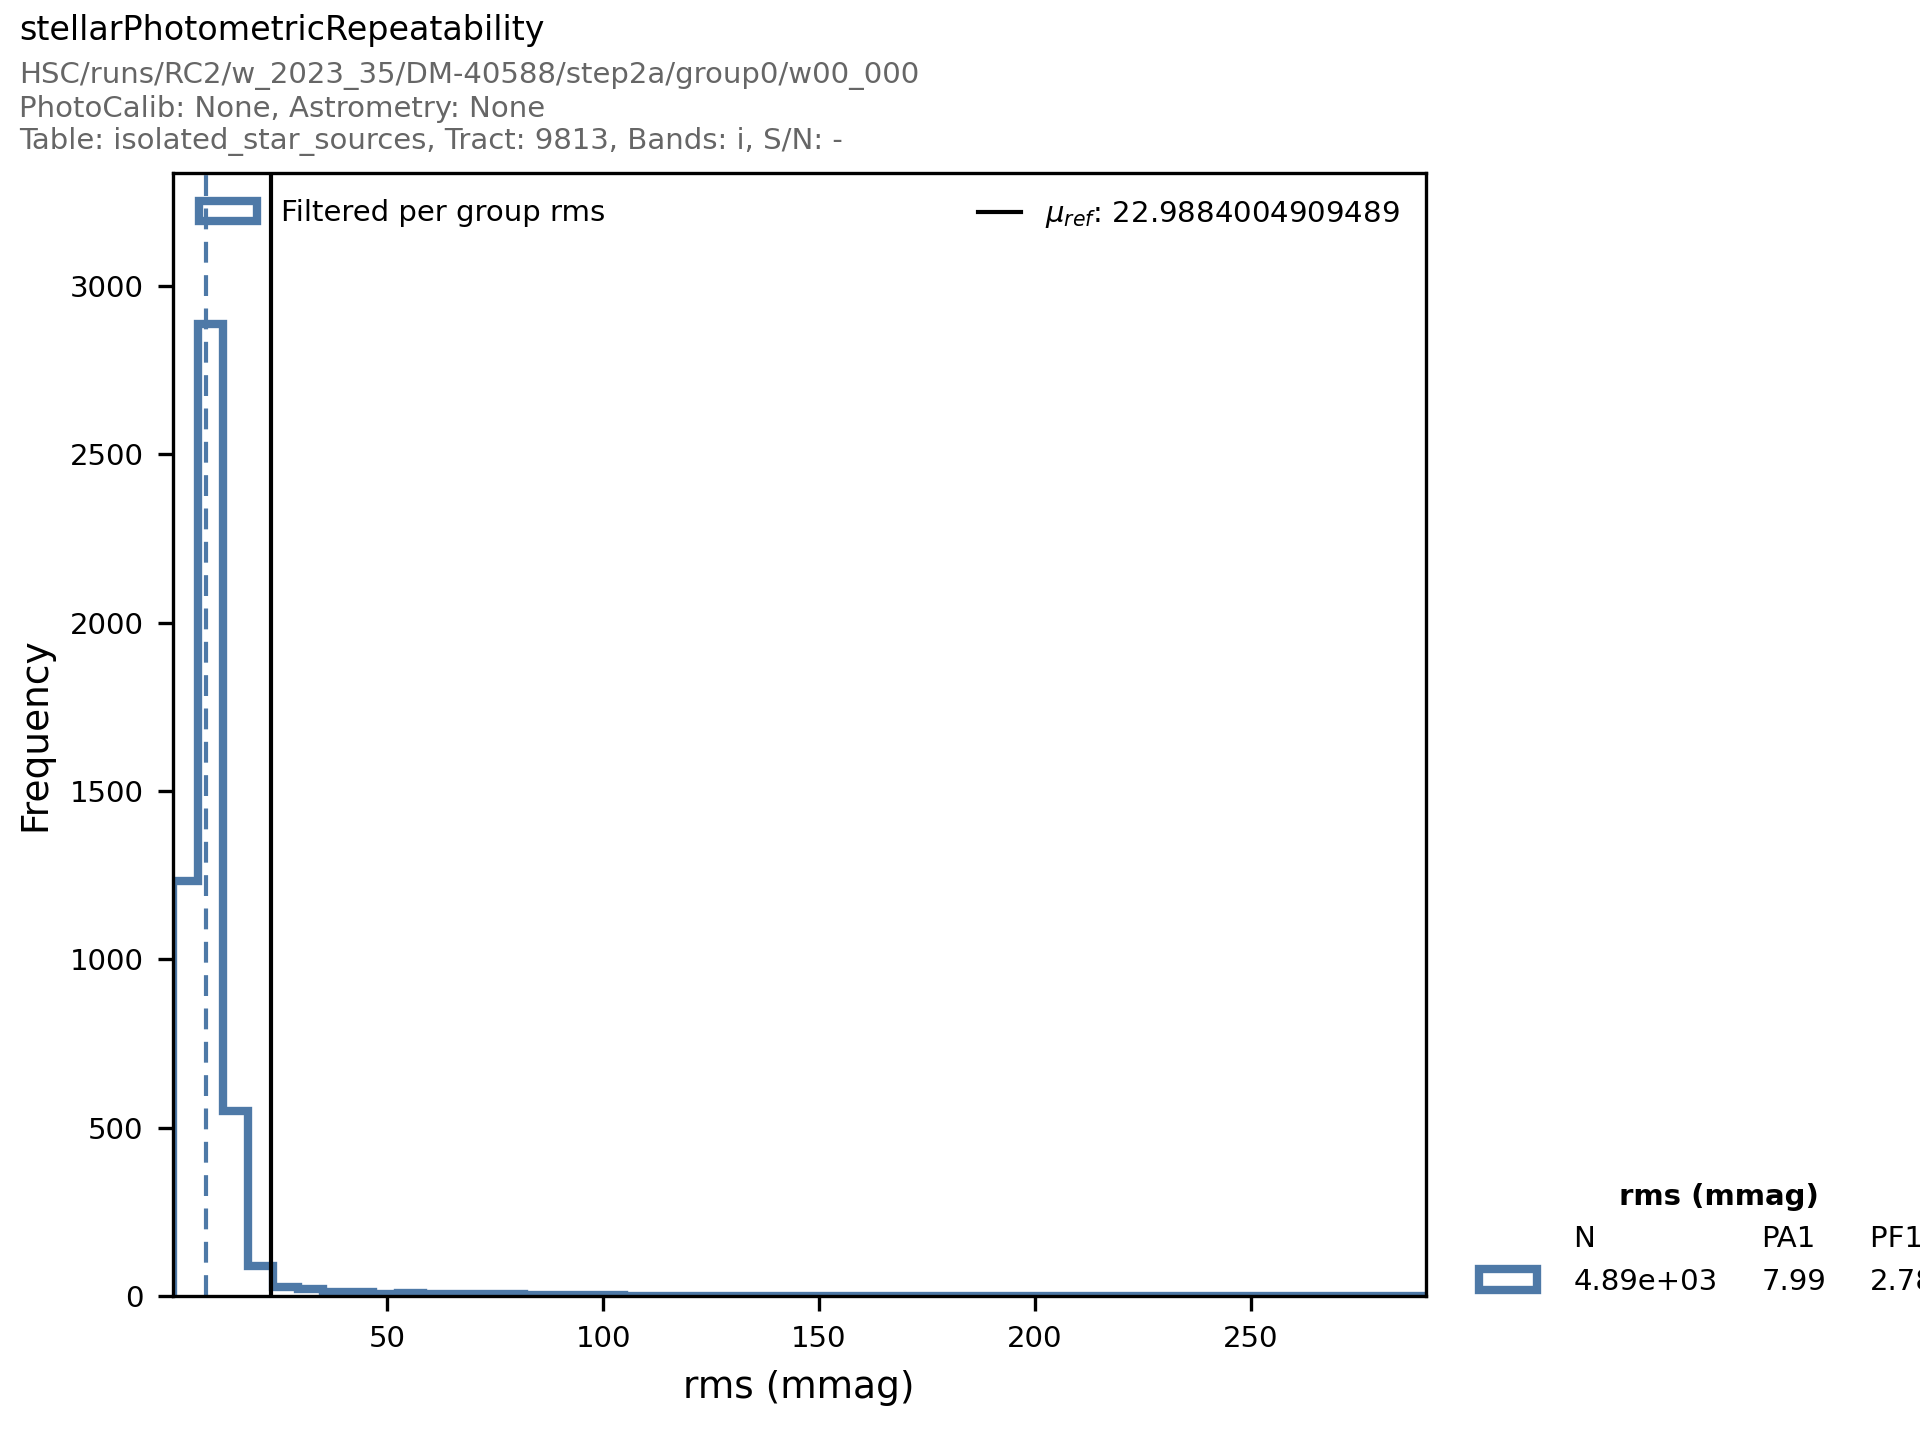
\includegraphics[width=4.66667in, ]{jira_imgs/4828.png}

}
\begin{tabular}{p{2cm}p{14cm}}
\toprule
Step 5 & Step Execution Status: \textbf{ Pass } \\ \hline
\end{tabular}
 Description \\
{\footnotesize
Change the value of the PA2 threshold in the pipeline yaml for
analysis\_tools, then rerun analysis\_tools

}
\hdashrule[0.5ex]{\textwidth}{1pt}{3mm}
  Expected Result \\
{\footnotesize

}
\hdashrule[0.5ex]{\textwidth}{1pt}{3mm}
  Actual Result \\
{\footnotesize
Changed the following line in matchedVisitQualityCore\_changePA2.yaml:\\
atools.stellarPhotometricRepeatability.PA2Value: 25.0\\
\strut \\
then executed:\\
pipetask -\/-long-log run -j 2 -b /repo/main -\/-register-dataset-types
-p matchedVisitQualityCore\_changePA2.yaml -d "band in
(\textquotesingle g\textquotesingle, \textquotesingle r\textquotesingle,
\textquotesingle i\textquotesingle) AND tract=9813 AND
skymap=\textquotesingle hsc\_rings\_v1\textquotesingle{} AND
instrument=\textquotesingle HSC\textquotesingle" -\/-output
u/jcarlin/pa2\_25 -i HSC/runs/RC2/w\_2023\_35/DM-40588 -\/-instrument
lsst.obs.subaru.HyperSuprimeCam 2\textgreater\&1 \textbar{} tee
w35\_2023\_tract9813\_pa2\_25.txt

}
\begin{tabular}{p{2cm}p{14cm}}
\toprule
Step 6 & Step Execution Status: \textbf{ Pass } \\ \hline
\end{tabular}
 Description \\
{\footnotesize
Confirm that the new PA2 threshold has been applied when computing PF1.

}
\hdashrule[0.5ex]{\textwidth}{1pt}{3mm}
  Expected Result \\
{\footnotesize
A JSON file (and/or a report generated from that JSON file)
demonstrating that PF1 has been calculated (and that it used the
requested threshold value of PA2gri).

}
\hdashrule[0.5ex]{\textwidth}{1pt}{3mm}
  Actual Result \\
{\footnotesize
Open a python terminal to check the results:\\
\strut \\
\textgreater\textgreater\textgreater{} from lsst.daf.butler import
Butler\\
\textgreater\textgreater\textgreater{}
repo=\textquotesingle/repo/main\textquotesingle{}\\
\textgreater\textgreater\textgreater{}
collection=\textquotesingle u/jcarlin/pa2\_25\textquotesingle{}\\
\textgreater\textgreater\textgreater{} butler = Butler(repo,
collections=collection)\\
\textgreater\textgreater\textgreater{} dataId =
\{\textquotesingle tract\textquotesingle:9813,
\textquotesingle instrument\textquotesingle:\textquotesingle HSC\textquotesingle,
\textquotesingle skymap\textquotesingle:\textquotesingle hsc\_rings\_v1\textquotesingle\}\\
\textgreater\textgreater\textgreater{} metrics =
butler.get(\textquotesingle matchedVisitCore\_metrics\textquotesingle,
dataId=dataId)\\
\textgreater\textgreater\textgreater{} for m in
metrics{[}\textquotesingle stellarPhotometricRepeatability\textquotesingle{]}:\\
... ~ ~~print(m)\\
...~\\
g\_stellarPhotRepeatStdev: 6.979476571776661 mmag\\
g\_stellarPhotRepeatOutlierFraction: 3.1032885595182953 \%\\
g\_ct: 2159.0 ct\\
r\_stellarPhotRepeatStdev: 8.902557135179485 mmag\\
r\_stellarPhotRepeatOutlierFraction: 3.07610713338637 \%\\
r\_ct: 3771.0 ct\\
i\_stellarPhotRepeatStdev: 7.9884004909489015 mmag\\
i\_stellarPhotRepeatOutlierFraction: 1.859799713876967 \%\\
i\_ct: 4893.0 ct\\
z\_stellarPhotRepeatStdev: nan mmag\\
z\_stellarPhotRepeatOutlierFraction: nan \%\\
z\_ct: 0.0 ct\\
y\_stellarPhotRepeatStdev: nan mmag\\
y\_stellarPhotRepeatOutlierFraction: nan \%\\
y\_ct: 0.0 ct\\
\textgreater\textgreater\textgreater{} metrics\_config =
butler.get(\textquotesingle analyzeMatchedVisitCore\_config\textquotesingle,
dataId=dataId)\\
\textgreater\textgreater\textgreater{} config\_dict =
metrics\_config.toDict()\\
\textgreater\textgreater\textgreater{}
config\_dict{[}\textquotesingle atools\textquotesingle{]}{[}\textquotesingle stellarPhotometricRepeatability\textquotesingle{]}{[}\textquotesingle process\textquotesingle{]}{[}\textquotesingle calculateActions\textquotesingle{]}{[}\textquotesingle photRepeatOutlier\textquotesingle{]}\\
\{\textquotesingle op\textquotesingle:
\textquotesingle ge\textquotesingle,
\textquotesingle threshold\textquotesingle: 25.0,
\textquotesingle vectorKey\textquotesingle:
\textquotesingle perGroupStdevFiltered\textquotesingle,
\textquotesingle percent\textquotesingle: True,
\textquotesingle relative\_to\_median\textquotesingle: True\}\\
\strut \\
We can see from both the butler artifacts seen above, and the figure
below, that the threshold PA2 has been set to 25.0 mmag from the
measured PA1 value, as requested.\\
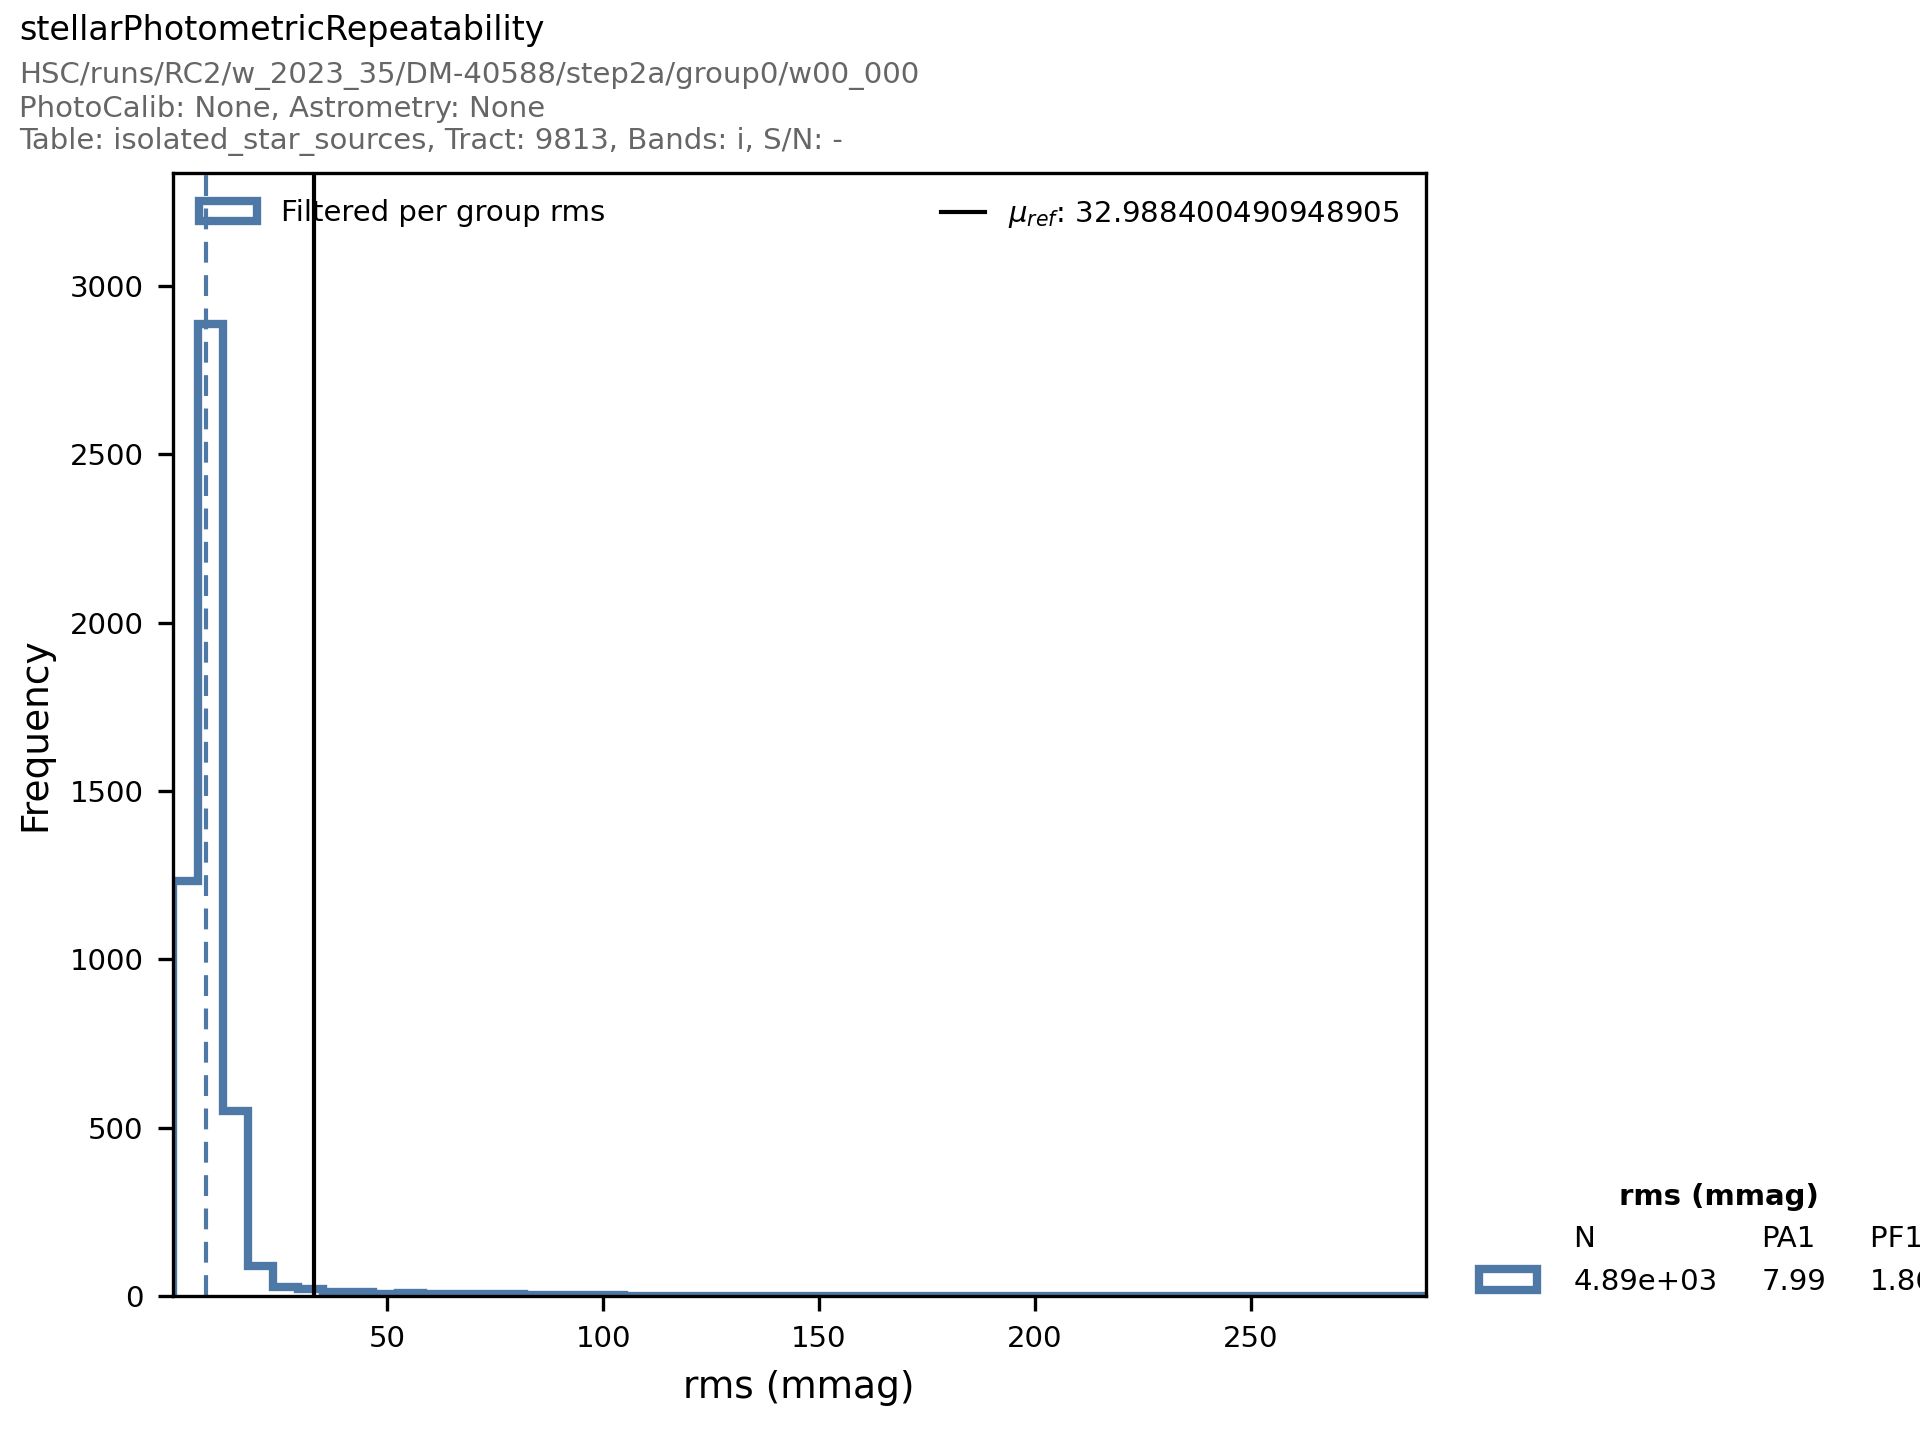
\includegraphics[width=4.26042in, ]{jira_imgs/4829.png}We
have thus demonstrated that the repeatability outlier limit PA2 can be
applied for the gri bands.

}

\paragraph{ LVV-T1758 - Verify that the repeatability outlier limit for isolated bright
non-saturated point sources in the u, z, and y filters (PA2uzy) can be
applied. }\mbox{}\\

Version \textbf{1}.
Status \textbf{Approved}.
Open  \href{https://jira.lsstcorp.org/secure/Tests.jspa#/testCase/LVV-T1758}{\textit{ LVV-T1758 } }
test case in Jira.

Verify that the DM system has provided the code to apply the
repeatability outlier limit for isolated bright non-saturated point
sources in the u, z, and y filters(PA2uzy) to computed values of the PF1
metric.

\textbf{ Preconditions}:\\


Execution status: {\bf Pass }

Final comment:\\Note that because we do not have access to u-band data, this test was
performed for only y- and z-band. The steps would be unchanged for
u-band data.


Detailed steps results:

\begin{tabular}{p{2cm}p{14cm}}
\toprule
Step 1 & Step Execution Status: \textbf{ Pass } \\ \hline
\end{tabular}
 Description \\
{\footnotesize
Identify a dataset containing at least one field in each of the u, z,
and y filters with multiple overlapping visits.

}
\hdashrule[0.5ex]{\textwidth}{1pt}{3mm}
  Expected Result \\
{\footnotesize
A dataset that has been ingested into a Butler repository.

}
\hdashrule[0.5ex]{\textwidth}{1pt}{3mm}
  Actual Result \\
{\footnotesize
For this test we use the most recent reprocessing of the Subaru+HSC RC2
dataset. The data were processed with the w\_2023\_35 pipelines.

}
\begin{tabular}{p{2cm}p{14cm}}
\toprule
Step 2 & Step Execution Status: \textbf{ Pass } \\ \hline
\end{tabular}
 Description \\
{\footnotesize
The `path` that you will use depends on where you are running the
science pipelines. Options:\\
\strut \\

\begin{itemize}
\tightlist
\item
  local (newinstall.sh - based
  install):{[}path\_to\_installation{]}/loadLSST.bash
\item
  development cluster ("lsst-dev"): /software/lsstsw/stack/loadLSST.bash
\item
  LSP Notebook aspect (from a terminal):
  /opt/lsst/software/stack/loadLSST.bash
\end{itemize}

\hfill\break
From the command line, execute the commands below in the example code:\\
\strut \\

}
\hdashrule[0.5ex]{\textwidth}{1pt}{3mm}
  Example Code \\
{\footnotesize
source `path`\\
setup lsst\_distrib

}
\hdashrule[0.5ex]{\textwidth}{1pt}{3mm}
  Expected Result \\
{\footnotesize
Science pipeline software is available for use. If additional packages
are needed (for example, \textquotesingle obs\textquotesingle{} packages
such as `obs\_subaru`), then additional `setup` commands will be
necessary.\\
\strut \\
To check versions in use, type:\\
eups list -s

}
\hdashrule[0.5ex]{\textwidth}{1pt}{3mm}
  Actual Result \\
{\footnotesize
Current weekly stack initialized:\\
\textbf{lsst\_distrib} g4213664e8e+7835acb1bb w\_latest current
w\_2023\_40 setup

}
\begin{tabular}{p{2cm}p{14cm}}
\toprule
Step 3 & Step Execution Status: \textbf{ Pass } \\ \hline
\end{tabular}
 Description \\
{\footnotesize
Execute `analysis\_tools` on a repository containing processed data.
Identify the path to the data, which we will call
\textquotesingle DATA/path\textquotesingle, then execute something
similar to the following (with paths, datasets, and flags replaced or
additionally specified as needed):

}
\hdashrule[0.5ex]{\textwidth}{1pt}{3mm}
  Example Code \\
{\footnotesize
pipetask -\/-long-log run -j 2 -b DATA/path/butler.yaml
-\/-register-dataset-types -p
\$ANALYSIS\_TOOLS\_DIR/pipelines/matchedVisitQualityCore.yaml -d "band
in (\textquotesingle g\textquotesingle,
\textquotesingle r\textquotesingle, \textquotesingle i\textquotesingle)
AND tract=9813 AND
skymap=\textquotesingle hsc\_rings\_v1\textquotesingle{} AND
instrument=\textquotesingle HSC\textquotesingle" -\/-output
u/username/atools\_metrics -i HSC/runs/RC2/w\_2023\_36 -\/-instrument
lsst.obs.subaru.HyperSuprimeCam 2\textgreater\&1 \textbar{} tee
w36\_2023\_tract9813\_atools.txt

}
\hdashrule[0.5ex]{\textwidth}{1pt}{3mm}
  Expected Result \\
{\footnotesize
The output collection (in this case, "u/username/atools\_metrics")
containing metric measurements and any associated extras and metadata is
available via the butler.

}
\hdashrule[0.5ex]{\textwidth}{1pt}{3mm}
  Actual Result \\
{\footnotesize
Changed the value of PA2 in matchedVisitQualityCore\_changePA2.yaml to
15.0:\\
atools.stellarPhotometricRepeatability.PA2Value: 15.0\\
\strut \\
Then, executed the pipeline as follows:\\
pipetask -\/-long-log run -j 2 -b /repo/main -\/-register-dataset-types
-p matchedVisitQualityCore\_changePA2.yaml -d "band in
(\textquotesingle z\textquotesingle, \textquotesingle y\textquotesingle)
AND tract=9813 AND
skymap=\textquotesingle hsc\_rings\_v1\textquotesingle{} AND
instrument=\textquotesingle HSC\textquotesingle" -\/-output
u/jcarlin/pa2\_15\_zy -i HSC/runs/RC2/w\_2023\_35/DM-40588
-\/-instrument lsst.obs.subaru.HyperSuprimeCam 2\textgreater\&1
\textbar{} tee w35\_2023\_tract9813\_zy\_pa2\_15.txt\\
\strut \\

}
\begin{tabular}{p{2cm}p{14cm}}
\toprule
Step 4 & Step Execution Status: \textbf{ Pass } \\ \hline
\end{tabular}
 Description \\
{\footnotesize
Confirm that the PA2uzy threshold has been applied to the assessment of
the computed values of PF1 for filters u,z,y.

}
\hdashrule[0.5ex]{\textwidth}{1pt}{3mm}
  Expected Result \\
{\footnotesize
A JSON file (and/or a report generated from that JSON file)
demonstrating that PF1 has been calculated (and that it used the
requested PA2uzy threshold).

}
\hdashrule[0.5ex]{\textwidth}{1pt}{3mm}
  Actual Result \\
{\footnotesize
Examine the results in a python terminal:\\
\strut \\
\textgreater\textgreater\textgreater{} from lsst.daf.butler import
Butler\\
\textgreater\textgreater\textgreater{}
repo=\textquotesingle/repo/main\textquotesingle{}\\
\textgreater\textgreater\textgreater{}
collection=\textquotesingle u/jcarlin/pa2\_15\_zy\textquotesingle{}\\
\textgreater\textgreater\textgreater{} butler = Butler(repo,
collections=collection)\\
\textgreater\textgreater\textgreater{} dataId =
\{\textquotesingle tract\textquotesingle:9813,
\textquotesingle instrument\textquotesingle:\textquotesingle HSC\textquotesingle,
\textquotesingle skymap\textquotesingle:\textquotesingle hsc\_rings\_v1\textquotesingle\}\\
\textgreater\textgreater\textgreater{} metrics =
butler.get(\textquotesingle matchedVisitCore\_metrics\textquotesingle,
dataId=dataId)\\
\textgreater\textgreater\textgreater{} for m in
metrics{[}\textquotesingle stellarPhotometricRepeatability\textquotesingle{]}:\\
... print(m)\\
...\\
z\_stellarPhotRepeatStdev: 6.924991284071611 mmag\\
z\_stellarPhotRepeatOutlierFraction: 1.9053231192300137 \%\\
z\_ct: 5091.0 ct\\
y\_stellarPhotRepeatStdev: 7.237368762721793 mmag\\
y\_stellarPhotRepeatOutlierFraction: 0.964371818912403 \%\\
y\_ct: 3733.0 ct\\
\textgreater\textgreater\textgreater{} metrics\_config =
butler.get(\textquotesingle analyzeMatchedVisitCore\_config\textquotesingle,
dataId=dataId)\\
\textgreater\textgreater\textgreater{} config\_dict =
metrics\_config.toDict()\\
\textgreater\textgreater\textgreater{}
config\_dict{[}\textquotesingle atools\textquotesingle{]}{[}\textquotesingle stellarPhotometricRepeatability\textquotesingle{]}{[}\textquotesingle process\textquotesingle{]}{[}\textquotesingle calculateActions\textquotesingle{]}{[}\textquotesingle photRepeatOutlier\textquotesingle{]}\\
\{\textquotesingle op\textquotesingle:
\textquotesingle ge\textquotesingle,
\textquotesingle threshold\textquotesingle: 15.0,
\textquotesingle vectorKey\textquotesingle:
\textquotesingle perGroupStdevFiltered\textquotesingle,
\textquotesingle percent\textquotesingle: True,
\textquotesingle relative\_to\_median\textquotesingle: True\}\\
\strut \\
The following figure is output by the pipeline. The threshold (vertical
black line) is set at 15 mmag above the measured PA1 value, as
expected.\\
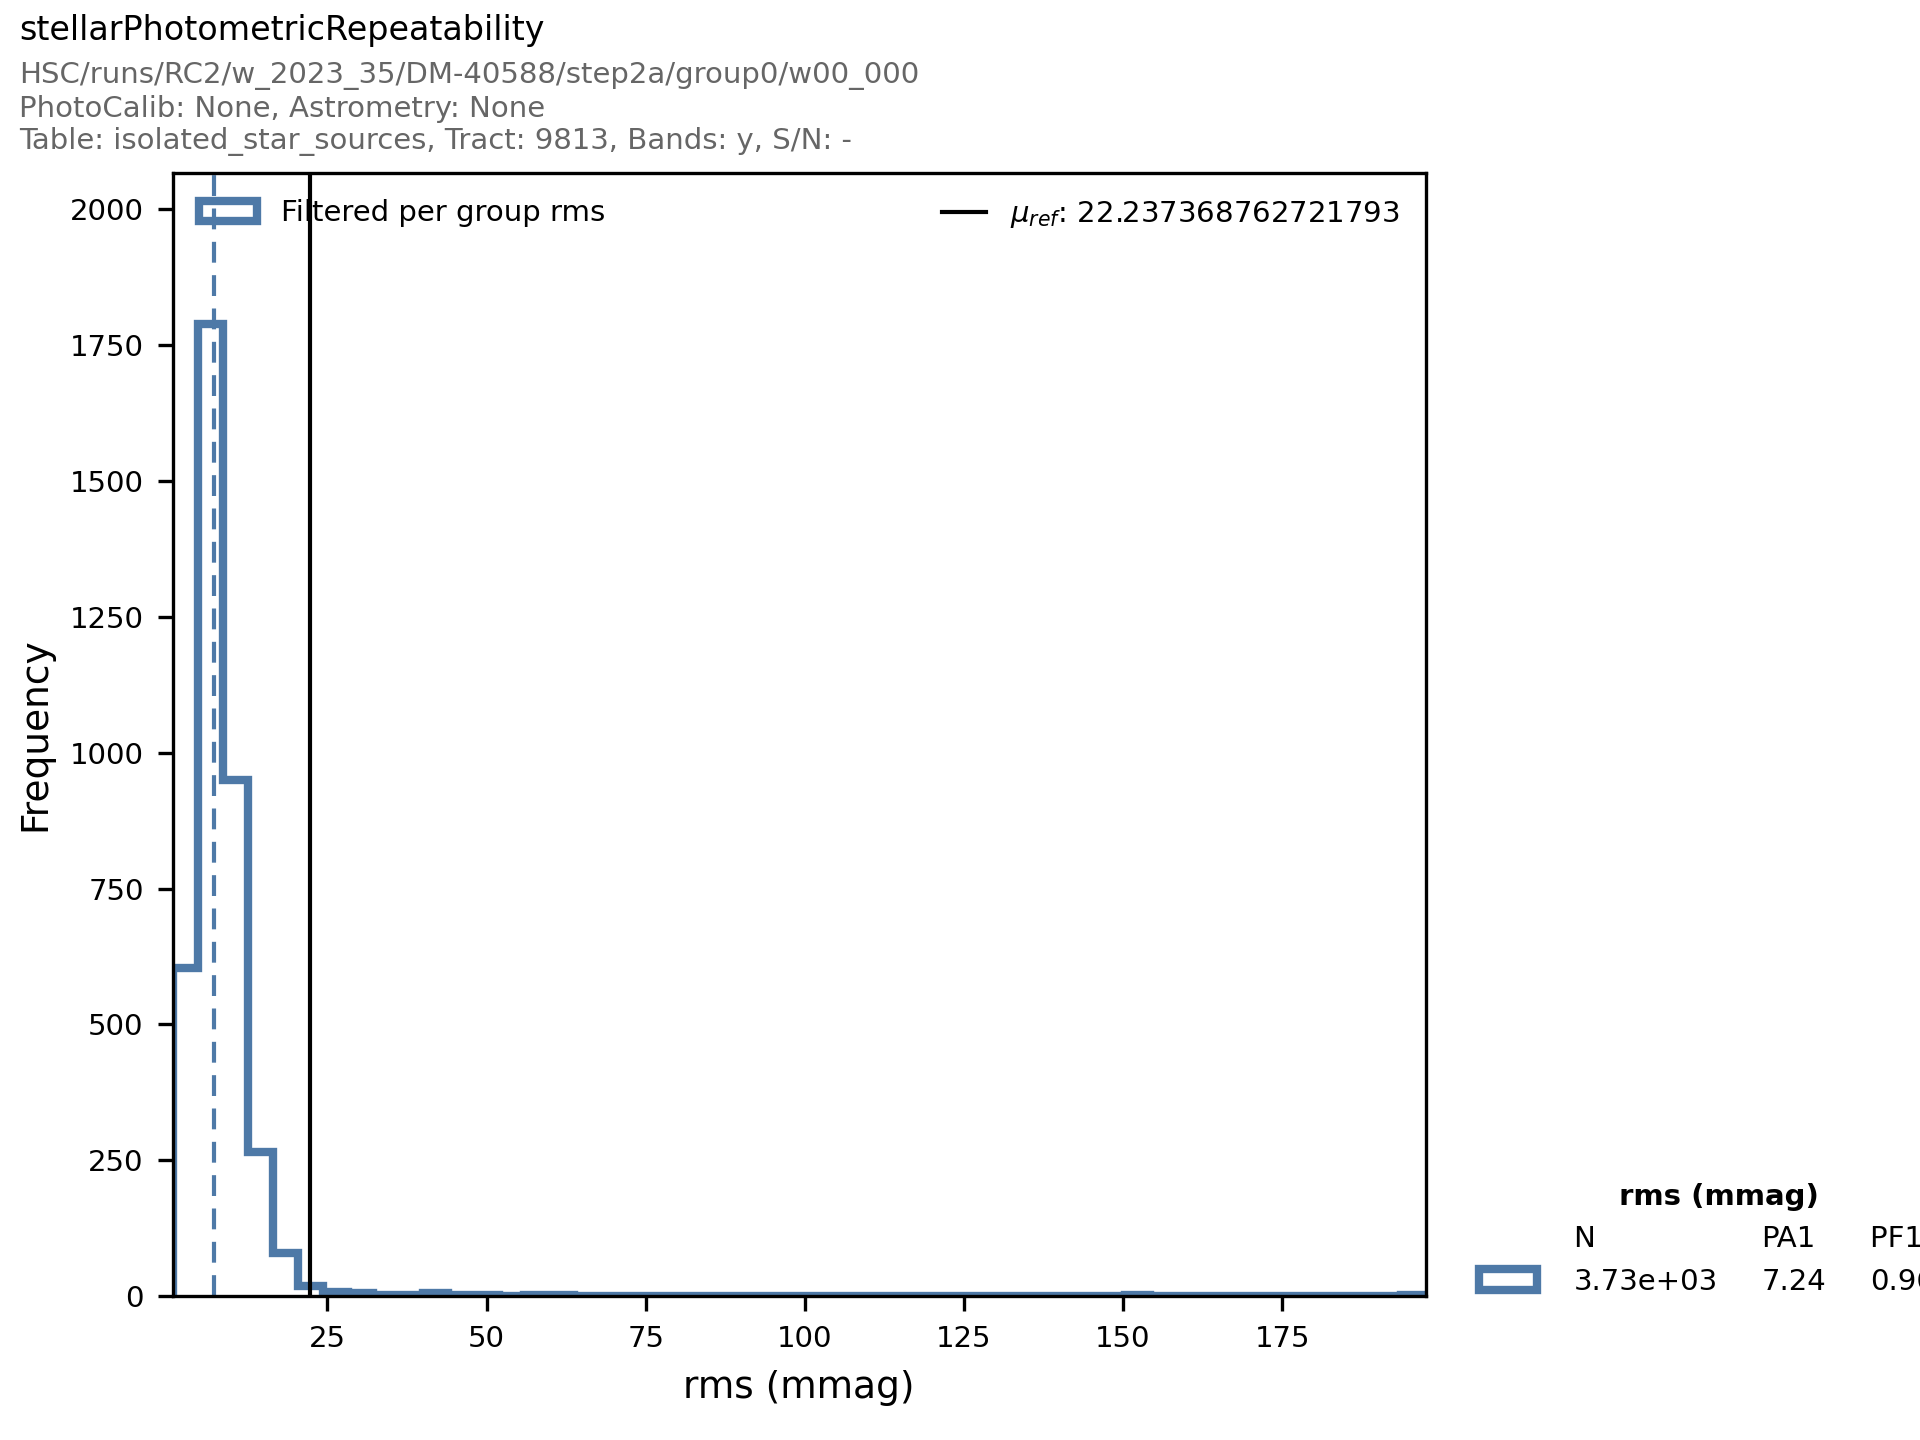
\includegraphics[width=4.33333in, ]{jira_imgs/4830.png}

}
\begin{tabular}{p{2cm}p{14cm}}
\toprule
Step 5 & Step Execution Status: \textbf{ Pass } \\ \hline
\end{tabular}
 Description \\
{\footnotesize
Change the value of the PA2 threshold in the pipeline yaml for
analysis\_tools, then rerun analysis\_tools

}
\hdashrule[0.5ex]{\textwidth}{1pt}{3mm}
  Expected Result \\
{\footnotesize

}
\hdashrule[0.5ex]{\textwidth}{1pt}{3mm}
  Actual Result \\
{\footnotesize
Changed the following line in matchedVisitQualityCore\_changePA2.yaml:\\
atools.stellarPhotometricRepeatability.PA2Value: 25.0\\
\strut \\
then executed:\\
pipetask -\/-long-log run -j 2 -b /repo/main -\/-register-dataset-types
-p matchedVisitQualityCore\_changePA2.yaml -d "band in
(\textquotesingle z\textquotesingle, \textquotesingle y\textquotesingle)
AND tract=9813 AND
skymap=\textquotesingle hsc\_rings\_v1\textquotesingle{} AND
instrument=\textquotesingle HSC\textquotesingle" -\/-output
u/jcarlin/pa2\_25\_zy -i HSC/runs/RC2/w\_2023\_35/DM-40588
-\/-instrument lsst.obs.subaru.HyperSuprimeCam 2\textgreater\&1
\textbar{} tee w35\_2023\_tract9813\_zy\_pa2\_25.txt\\
\strut \\

}
\begin{tabular}{p{2cm}p{14cm}}
\toprule
Step 6 & Step Execution Status: \textbf{ Pass } \\ \hline
\end{tabular}
 Description \\
{\footnotesize
Confirm that the new PA2 threshold has been applied when computing PF1.

}
\hdashrule[0.5ex]{\textwidth}{1pt}{3mm}
  Expected Result \\
{\footnotesize
A JSON file (and/or a report generated from that JSON file)
demonstrating that PF1 has been calculated (and that it used the
requested threshold value of PA2gri).

}
\hdashrule[0.5ex]{\textwidth}{1pt}{3mm}
  Actual Result \\
{\footnotesize
\textgreater\textgreater\textgreater{} from lsst.daf.butler import
Butler\\
\textgreater\textgreater\textgreater{}
repo=\textquotesingle/repo/main\textquotesingle{}\\
\textgreater\textgreater\textgreater{}
collection=\textquotesingle u/jcarlin/pa2\_15\_zy\textquotesingle{}\\
\textgreater\textgreater\textgreater{} butler = Butler(repo,
collections=collection)\\
\textgreater\textgreater\textgreater{} dataId =
\{\textquotesingle tract\textquotesingle:9813,
\textquotesingle instrument\textquotesingle:\textquotesingle HSC\textquotesingle,
\textquotesingle skymap\textquotesingle:\textquotesingle hsc\_rings\_v1\textquotesingle\}\\
\textgreater\textgreater\textgreater{} metrics =
butler.get(\textquotesingle matchedVisitCore\_metrics\textquotesingle,
dataId=dataId)\\
\textgreater\textgreater\textgreater{} for m in
metrics{[}\textquotesingle stellarPhotometricRepeatability\textquotesingle{]}:\\
... print(m)\\
...\\
z\_stellarPhotRepeatStdev: 6.924991284071611 mmag\\
z\_stellarPhotRepeatOutlierFraction: 1.9053231192300137 \%\\
z\_ct: 5091.0 ct\\
y\_stellarPhotRepeatStdev: 7.237368762721793 mmag\\
y\_stellarPhotRepeatOutlierFraction: 0.964371818912403 \%\\
y\_ct: 3733.0 ct\\
\textgreater\textgreater\textgreater{} metrics\_config =
butler.get(\textquotesingle analyzeMatchedVisitCore\_config\textquotesingle,
dataId=dataId)\\
\textgreater\textgreater\textgreater{} config\_dict =
metrics\_config.toDict()\\
\textgreater\textgreater\textgreater{}
config\_dict{[}\textquotesingle atools\textquotesingle{]}{[}\textquotesingle stellarPhotometricRepeatability\textquotesingle{]}{[}\textquotesingle process\textquotesingle{]}{[}\textquotesingle calculateActions\textquotesingle{]}{[}\textquotesingle photRepeatOutlier\textquotesingle{]}\\
\{\textquotesingle op\textquotesingle:
\textquotesingle ge\textquotesingle,
\textquotesingle threshold\textquotesingle: 25.0,
\textquotesingle vectorKey\textquotesingle:
\textquotesingle perGroupStdevFiltered\textquotesingle,
\textquotesingle percent\textquotesingle: True,
\textquotesingle relative\_to\_median\textquotesingle: True\}\\
\strut \\
We can see from both the butler artifacts seen above, and the figure
below, that the threshold PA2 has been set to 25.0 mmag from the
measured PA1 value, as requested.\\
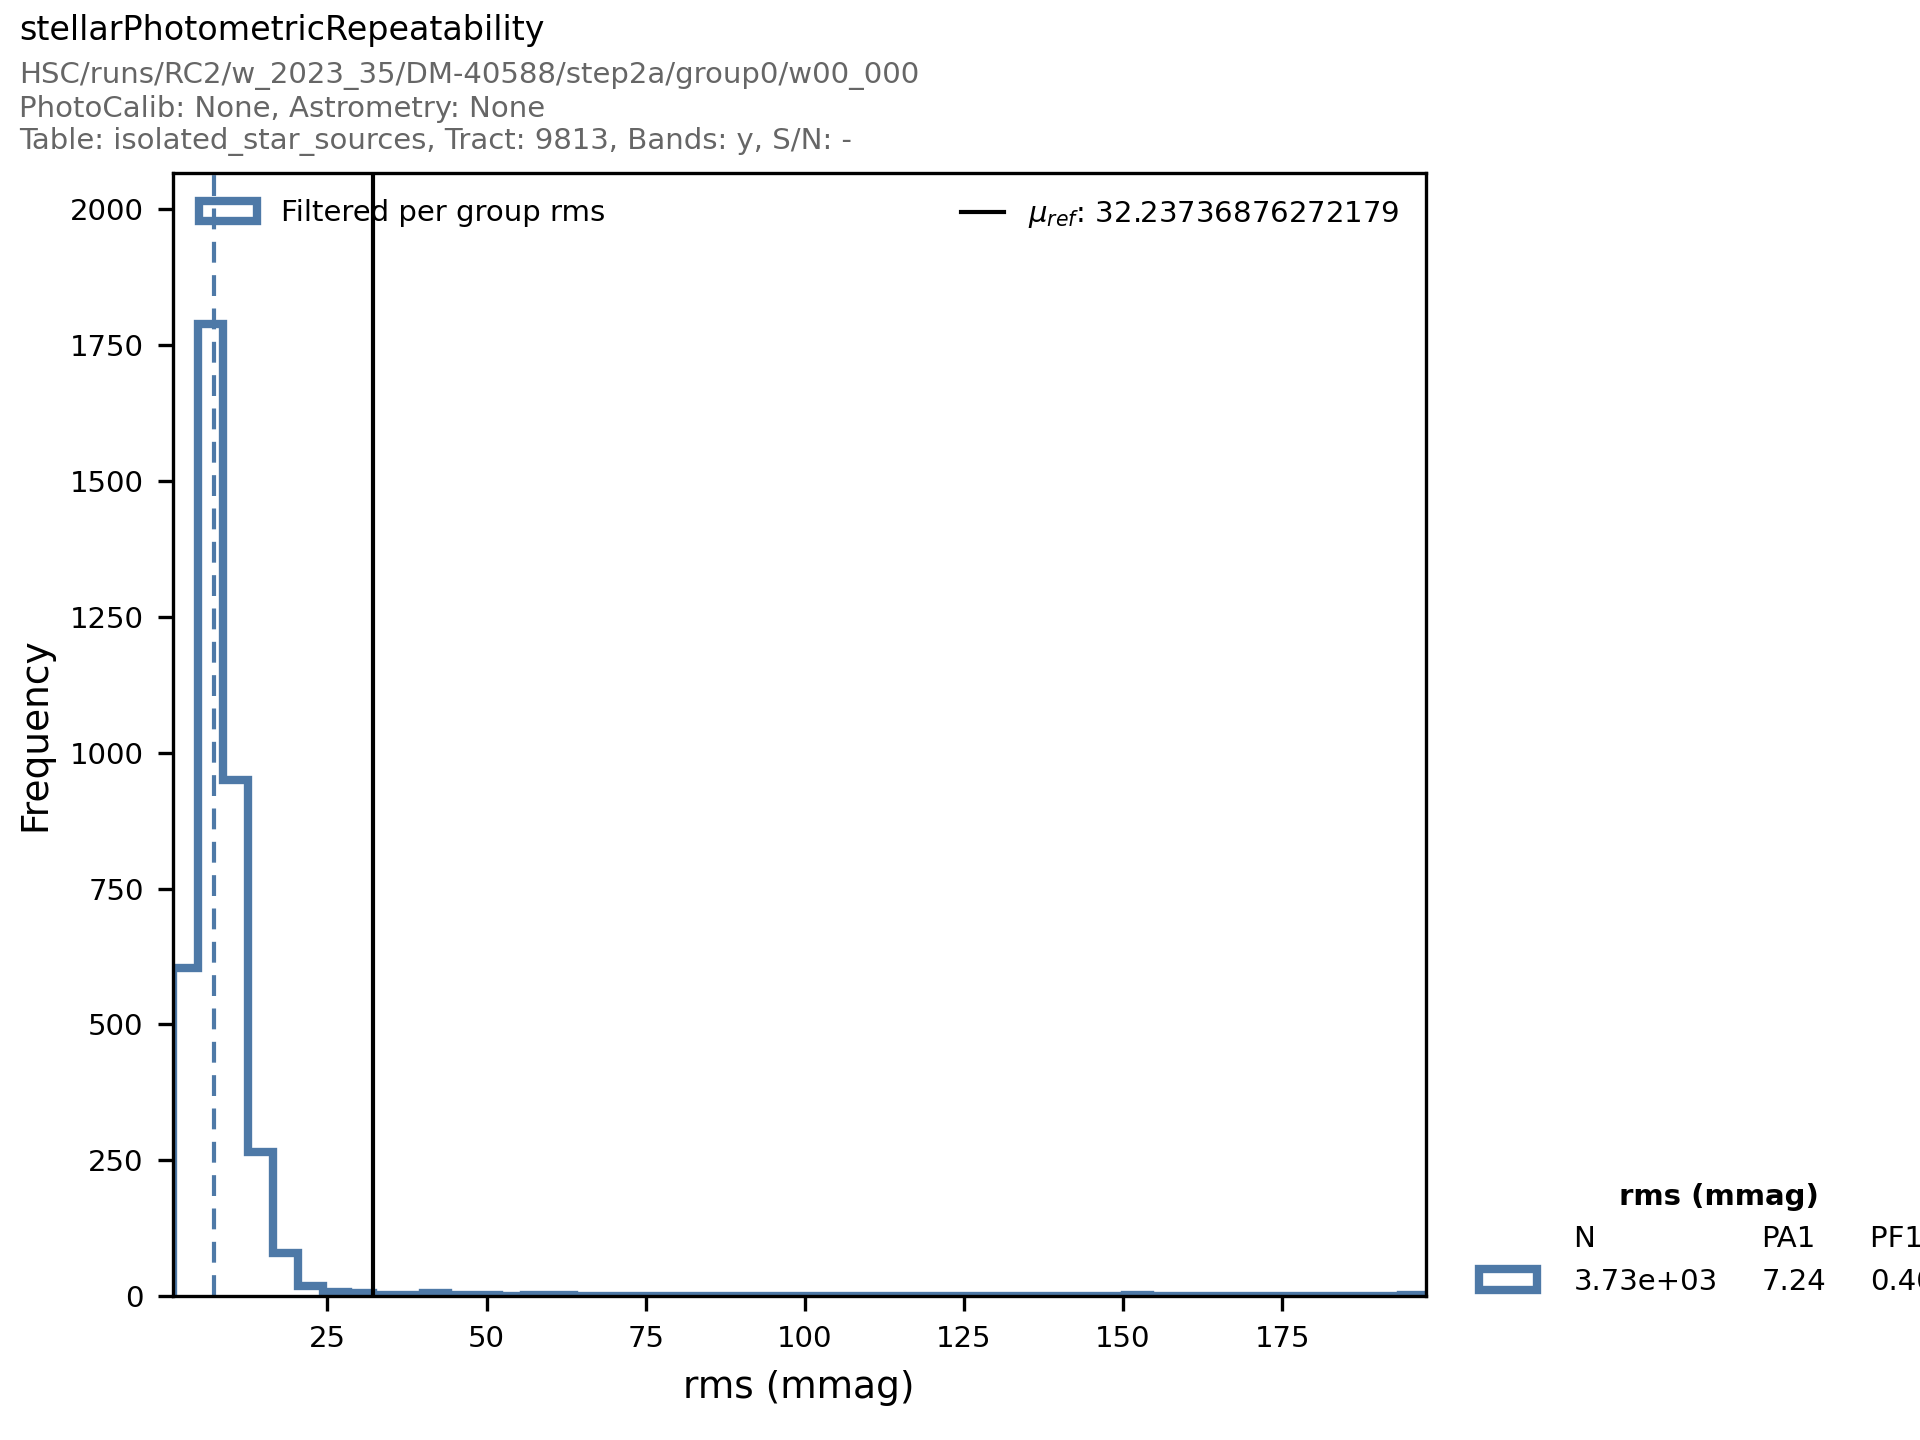
\includegraphics[width=4.48958in, ]{jira_imgs/4831.png}\\
We have thus demonstrated that the repeatability outlier limit PA2 can
be applied for the z and y bands.

}

\paragraph{ LVV-T149 - Verify implementation of Catalog Queries }\mbox{}\\

Version \textbf{1}.
Status \textbf{Approved}.
Open  \href{https://jira.lsstcorp.org/secure/Tests.jspa#/testCase/LVV-T149}{\textit{ LVV-T149 } }
test case in Jira.

Verify that SQL, or a similar structured language, can be used to query
catalogs.

\textbf{ Preconditions}:\\
An operational QSERV database that has been verified via
\href{https://jira.lsstcorp.org/secure/Tests.jspa\#/testCase/LVV-T1085}{LVV-T1085}
and
\href{https://jira.lsstcorp.org/secure/Tests.jspa\#/testCase/LVV-T1086}{LVV-T1086}
and
\href{https://jira.lsstcorp.org/secure/Tests.jspa\#/testCase/LVV-T1087}{LVV-T1087}.

Execution status: {\bf Pass }

Final comment:\\Executed using the IDF Notebook, Portal, and API aspects. For the
notebook execution, we used science pipelines version w\_2023\_34.


Detailed steps results:

\begin{tabular}{p{2cm}p{14cm}}
\toprule
Step 1 & Step Execution Status: \textbf{ Pass } \\ \hline
\end{tabular}
 Description \\
{\footnotesize
Execute a simple query (for example, the one below) and confirm that it
returns the expected result.

}
\hdashrule[0.5ex]{\textwidth}{1pt}{3mm}
  Example Code \\
{\footnotesize
SELECT * FROM dp02\_dc2\_catalogs.Object as obj WHERE
CONTAINS(POINT(\textquotesingle ICRS\textquotesingle, obj.coord\_ra,
obj.coord\_dec), CIRCLE(\textquotesingle ICRS\textquotesingle, 62.0,
-37.0, 0.10)) = 1

}
\hdashrule[0.5ex]{\textwidth}{1pt}{3mm}
  Expected Result \\
{\footnotesize
A catalog of objects satisfying the specified constraints. The catalog
should contain 26,115 results.

}
\hdashrule[0.5ex]{\textwidth}{1pt}{3mm}
  Actual Result \\
{\footnotesize
The query was executed in the notebook "test\_LVV-T149.ipynb" attached
to this document\textquotesingle s Github repository. The query executed
successfully in the notebook, and returned 26,115 results, as expected.

}
\begin{tabular}{p{2cm}p{14cm}}
\toprule
Step 2 & Step Execution Status: \textbf{ Pass } \\ \hline
\end{tabular}
 Description \\
{\footnotesize
Repeat the query from all available access routes (e.g., an external VO
client, the Science Platform query tool, and from within the Notebook
Aspect), confirming in each case that the results are as expected.

}
\hdashrule[0.5ex]{\textwidth}{1pt}{3mm}
  Expected Result \\
{\footnotesize

}
\hdashrule[0.5ex]{\textwidth}{1pt}{3mm}
  Actual Result \\
{\footnotesize
The Notebook query was demonstrated in step 1.\\
\strut \\
To query via the API aspect, we use Topcat, entering
"https://data.lsst.cloud/api/tap/" in the "Select TAP service" window as
seen below. (Note that the user has already set up an access token for
Topcat to access the RSP.)\\
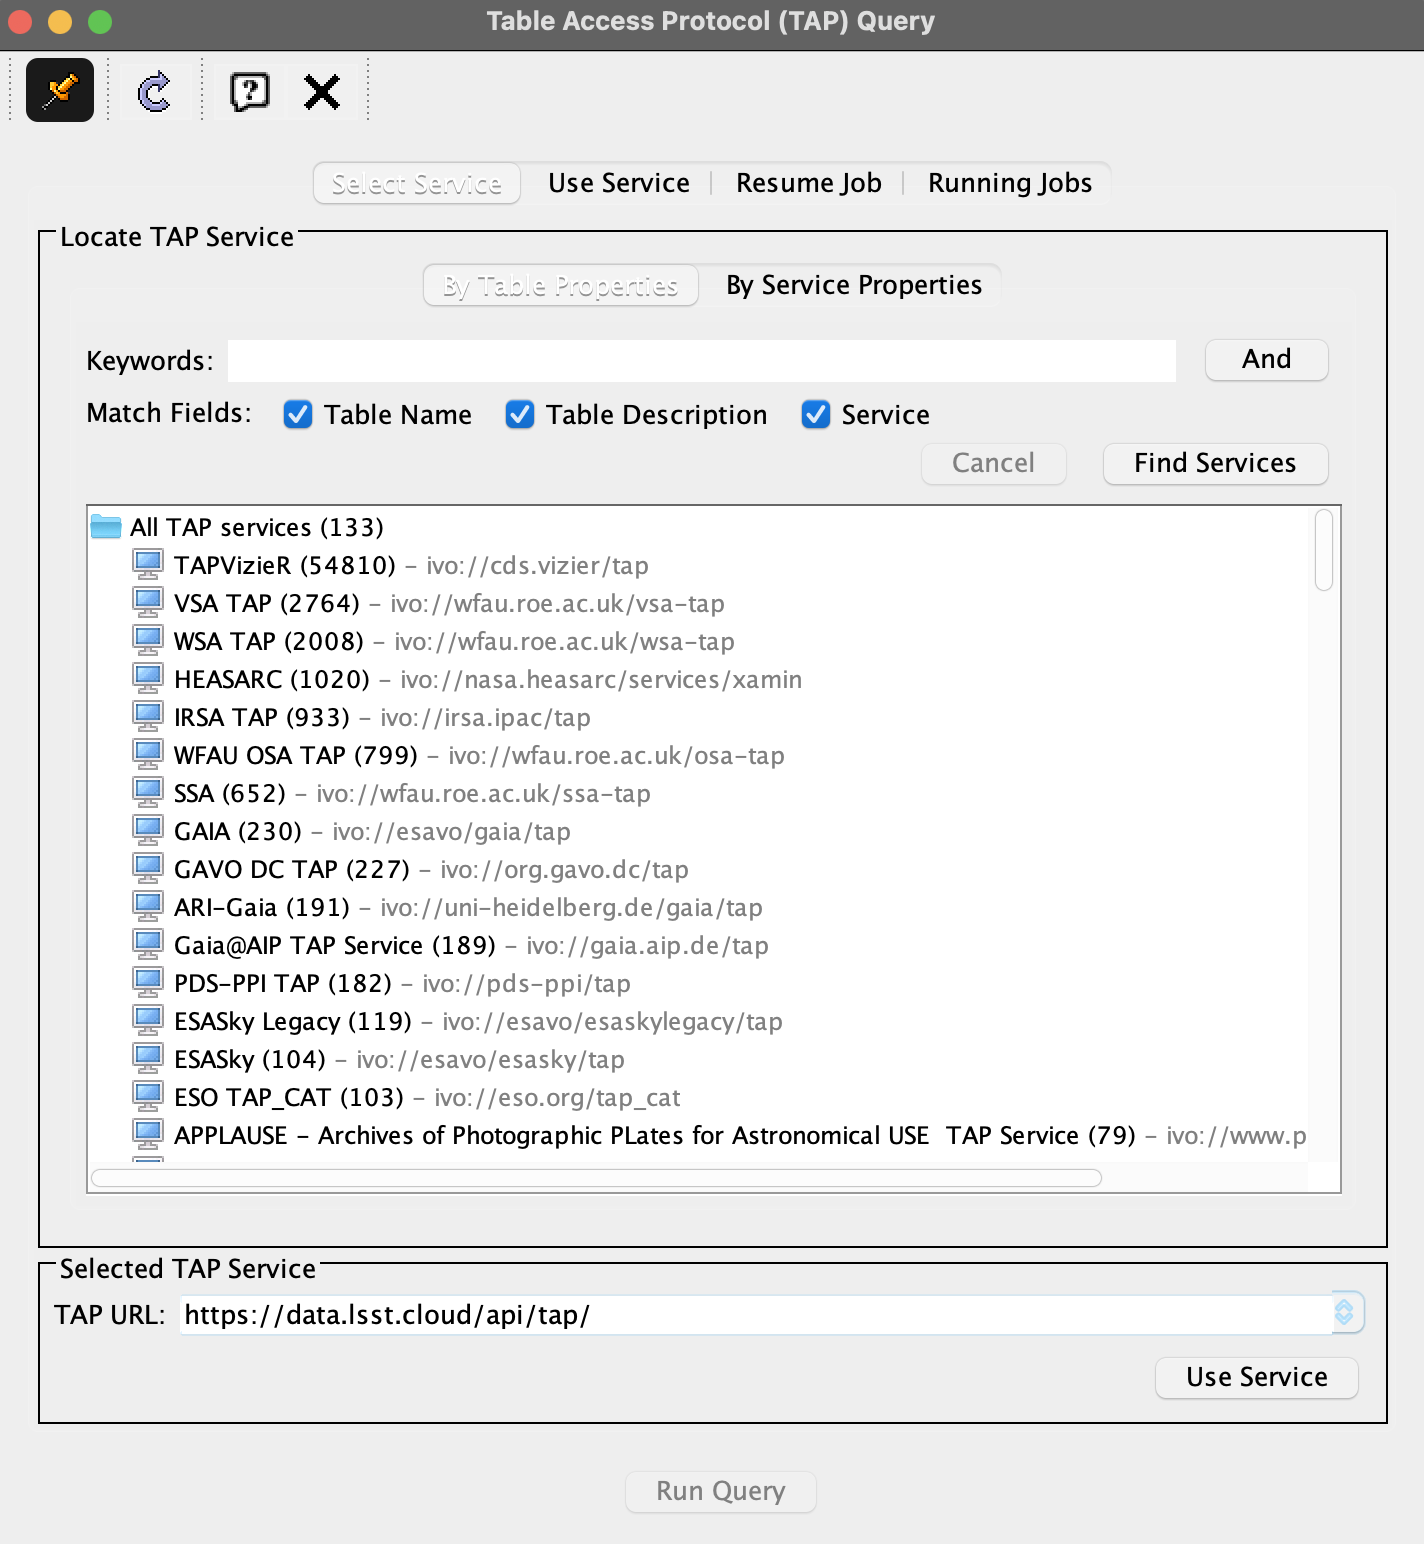
\includegraphics[width=3.79167in, ]{jira_imgs/4609.png}Next
we execute the query from the "Use Service" window as follows:\\
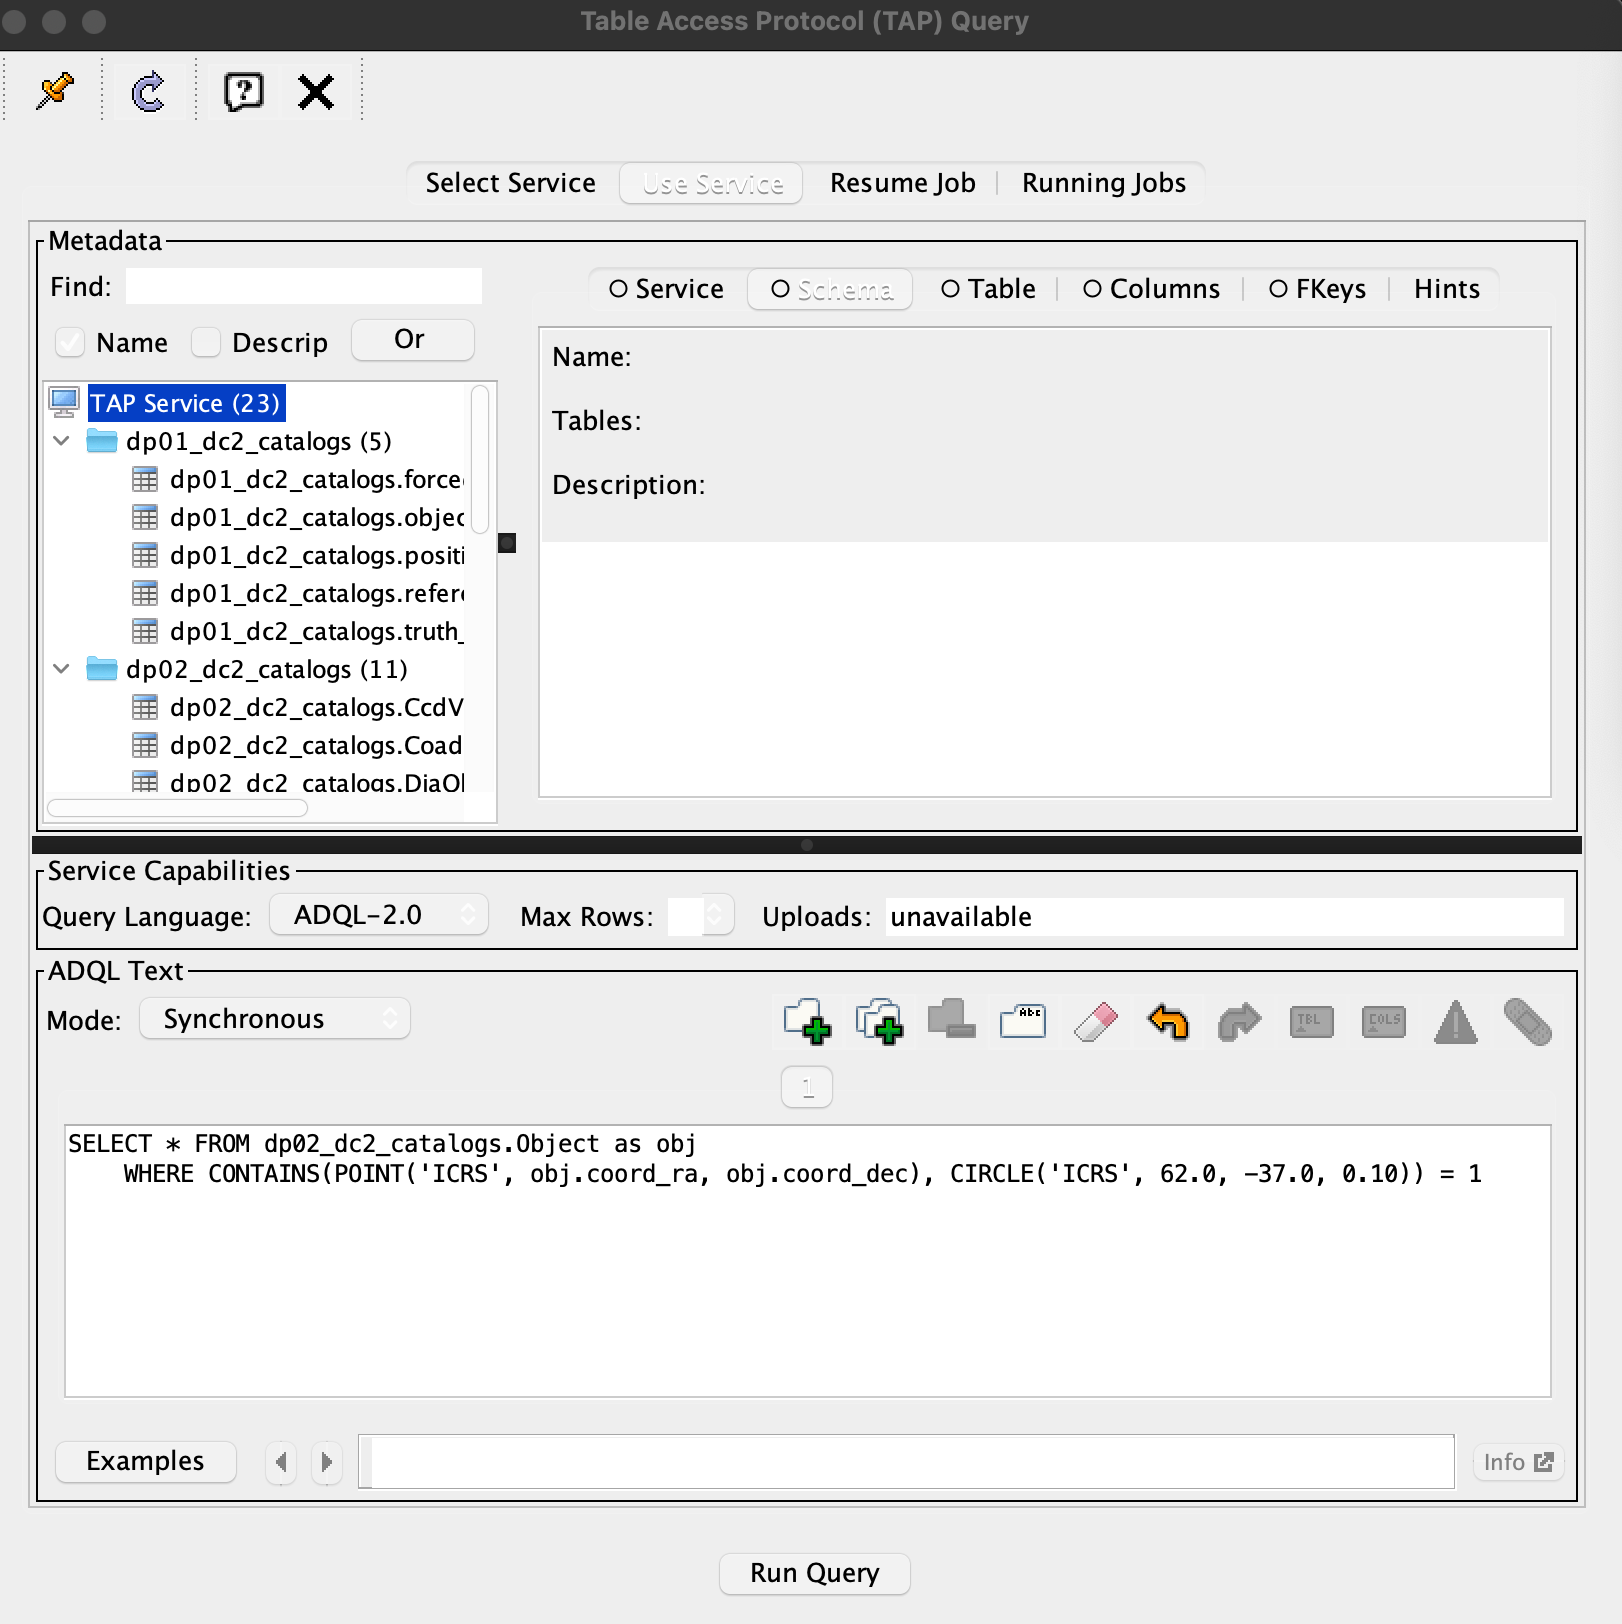
\includegraphics[width=4.41667in, ]{jira_imgs/4610.png}The
following screenshot shows that the query returned 26,115 results (and
991 columns of data), as expected.\\
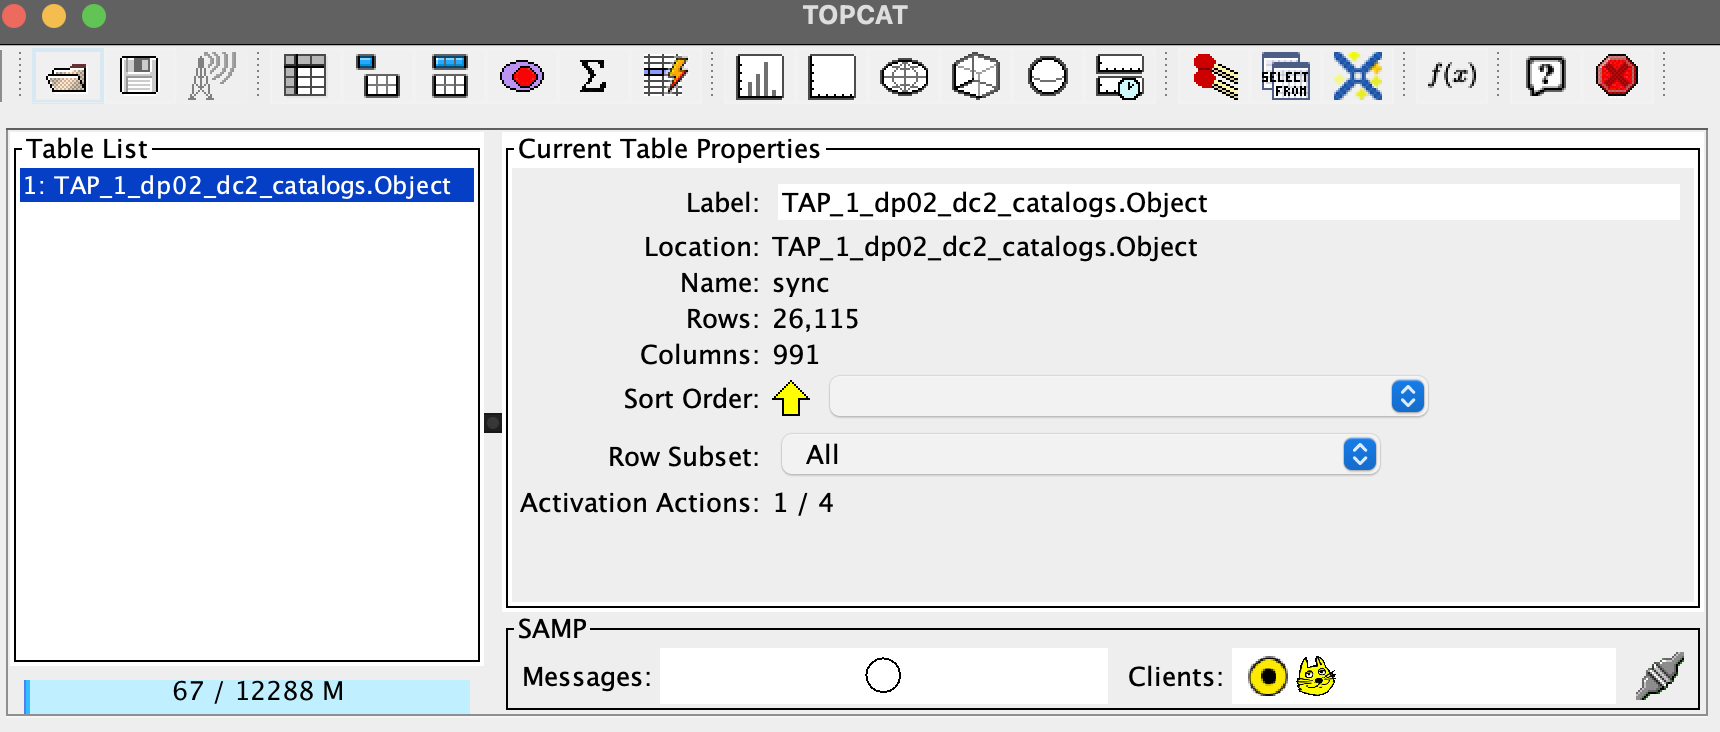
\includegraphics[width=4.78125in, ]{jira_imgs/4611.png}\\
Next we execute the same query from the RSP Portal aspect.\\
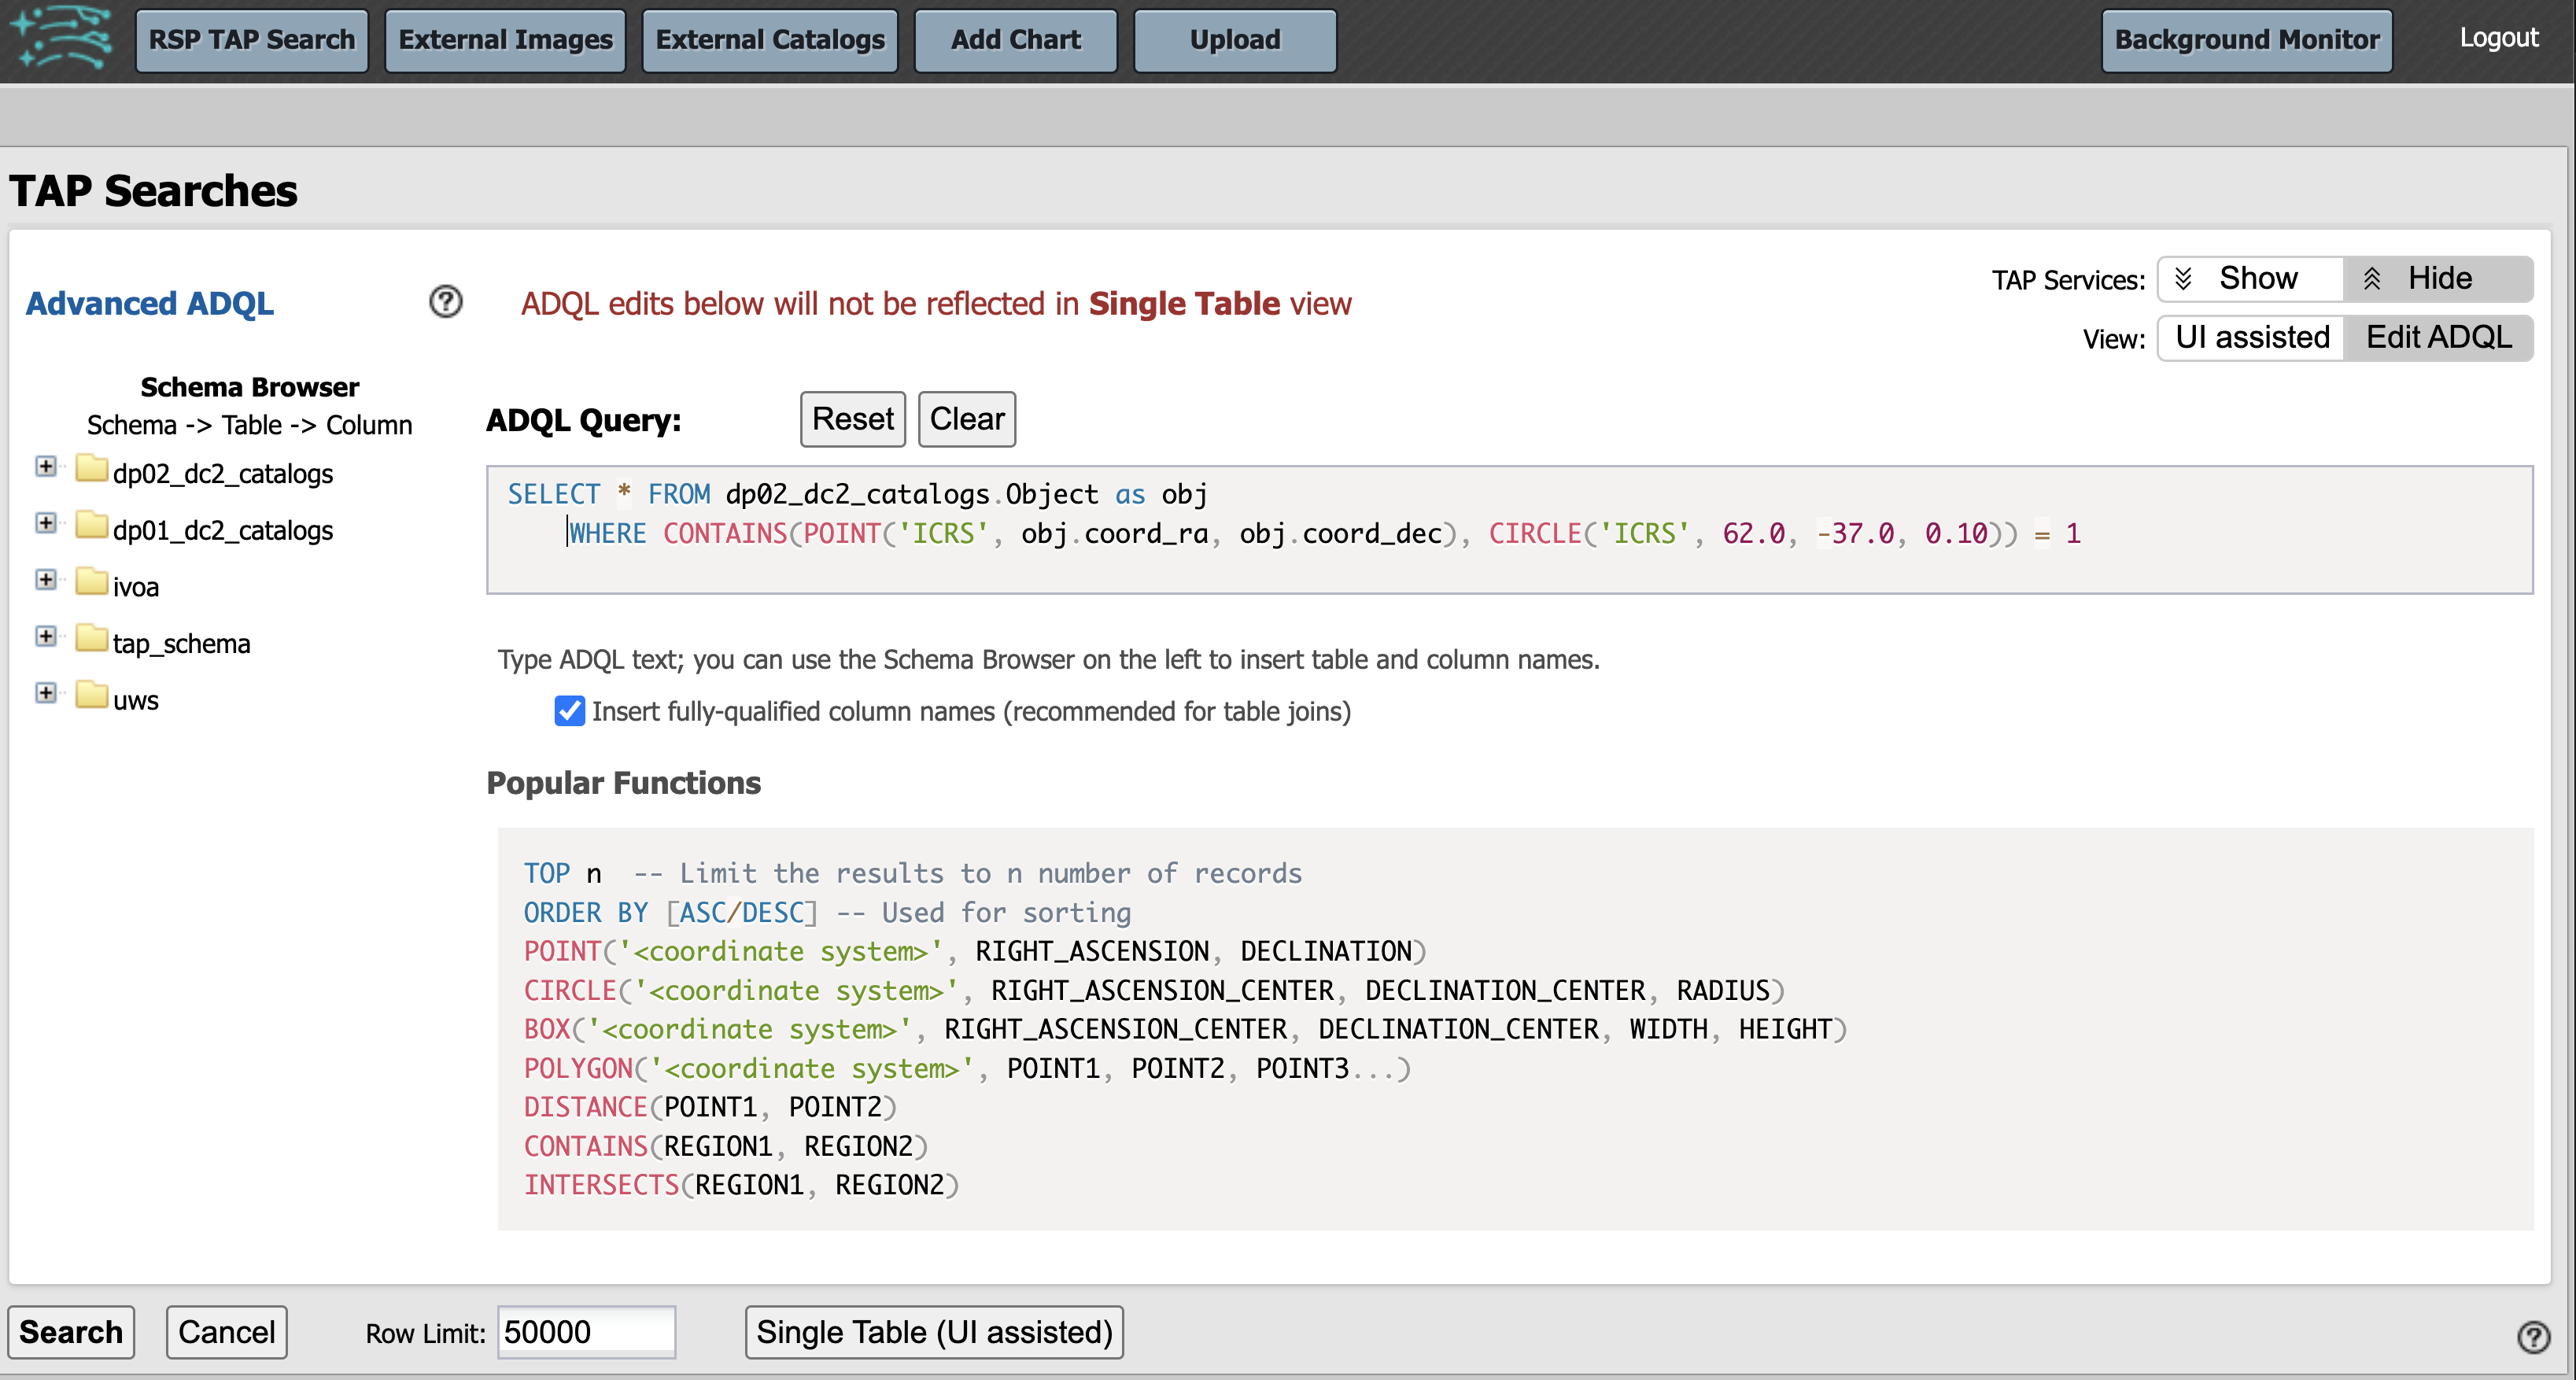
\includegraphics[width=5.16667in, ]{jira_imgs/4612.png}The
following screenshot shows the results, verifying that the query
returned 26,115 results, as expected.\\
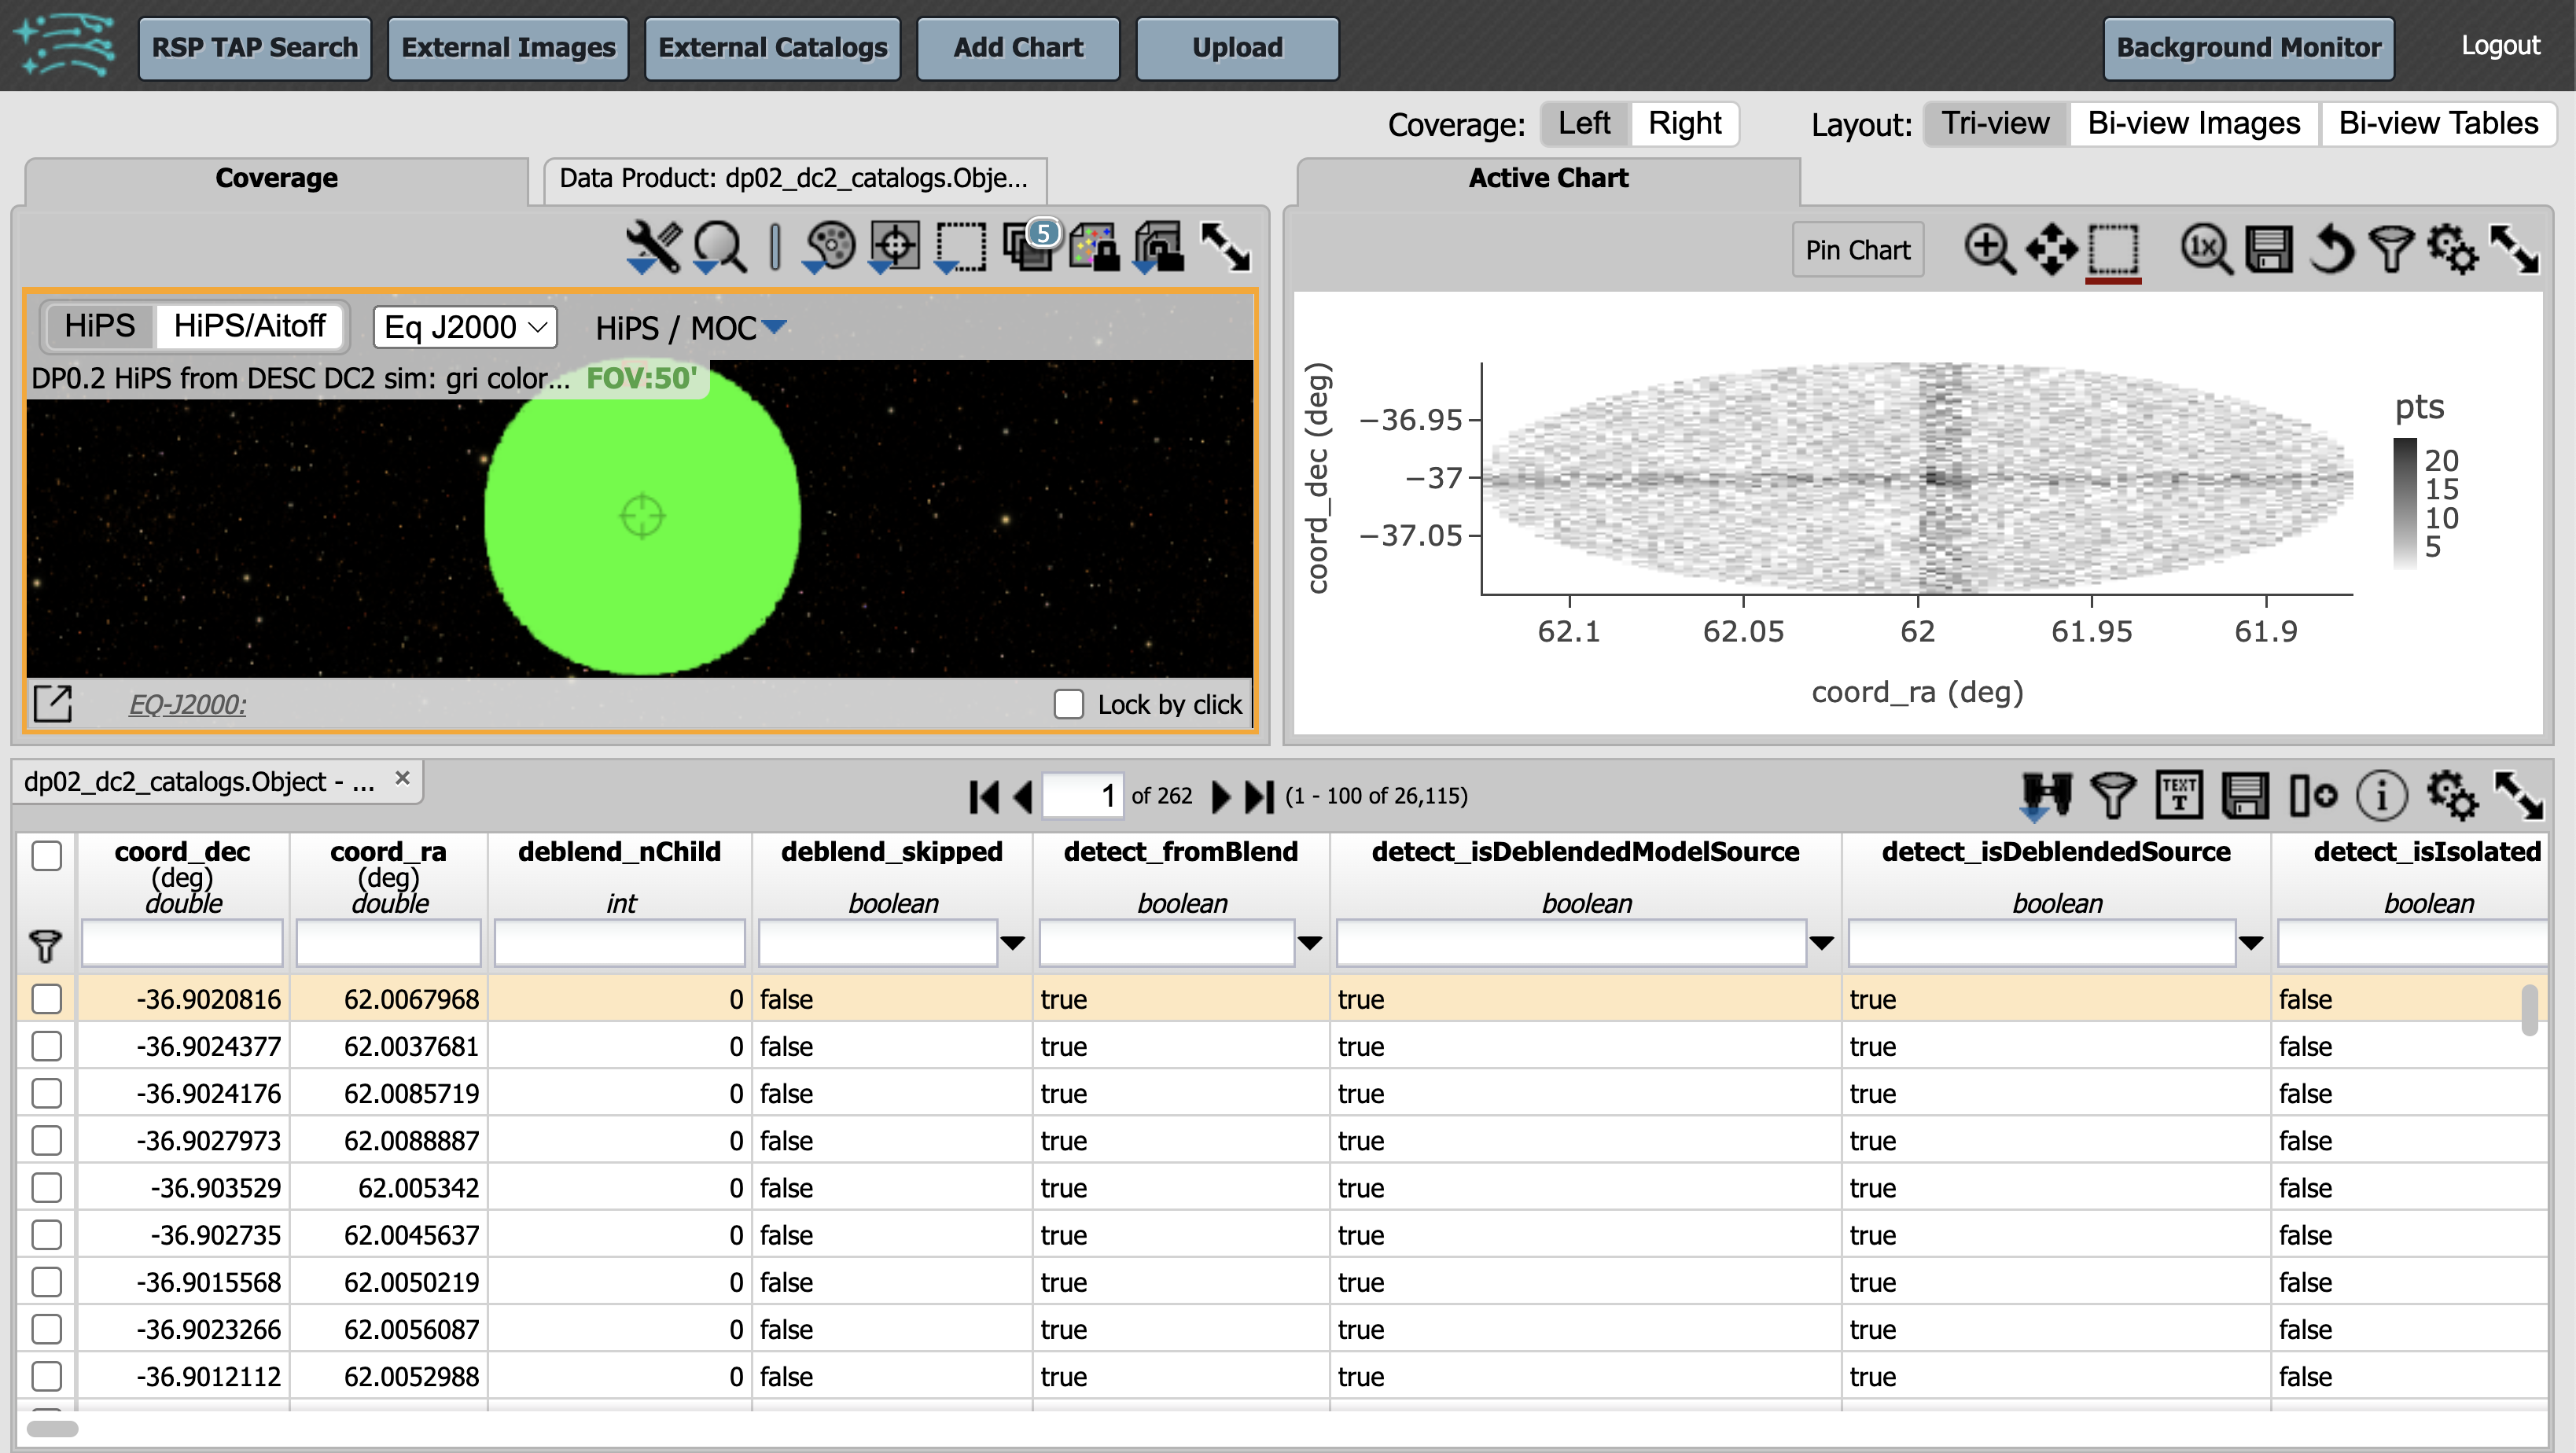
\includegraphics[width=5.20833in, ]{jira_imgs/4613.png}\\
We have thus demonstrated that catalogs can be queried via the Notebook,
Portal, and API aspects using ADQL queries.

}

\paragraph{ LVV-T40 - Verify implementation of Generate WCS for Visit Images }\mbox{}\\

Version \textbf{1}.
Status \textbf{Approved}.
Open  \href{https://jira.lsstcorp.org/secure/Tests.jspa#/testCase/LVV-T40}{\textit{ LVV-T40 } }
test case in Jira.

Verify that Processed Visit Images produced by the AP and DRP pipelines
include FITS WCS accurate to specified \textbf{astrometricAccuracy} over
the bounds of the image.

\textbf{ Preconditions}:\\


Execution status: {\bf Pass }

Final comment:\\Test executed with science pipelines version w\_2023\_37 in the RSP
Notebook aspect at the USDF.\\
\strut \\
The executed notebook was saved in the repository associated with this
campaign's test report as ``notebooks/test\_LVV-T40\_T1240.ipynb''.


Detailed steps results:

\begin{tabular}{p{2cm}p{14cm}}
\toprule
Step 1 & Step Execution Status: \textbf{ Pass } \\ \hline
\end{tabular}
 Description \\
{\footnotesize
Identify an appropriate repo containing processed HSC data for this
test.

}
\hdashrule[0.5ex]{\textwidth}{1pt}{3mm}
  Expected Result \\
{\footnotesize
A dataset with Processed Visit Images available.

}
\hdashrule[0.5ex]{\textwidth}{1pt}{3mm}
  Actual Result \\
{\footnotesize
For this test we use the most recent reprocessing of the Subaru+HSC RC2
dataset. The data were processed with the w\_2023\_32 pipelines.

}
\begin{tabular}{p{2cm}p{14cm}}
\toprule
Step 2 & Step Execution Status: \textbf{ Pass } \\ \hline
\end{tabular}
 Description \\
{\footnotesize
Identify the path to the data repository, which we will refer to as
\textquotesingle DATA/path\textquotesingle, then execute the following:

}
\hdashrule[0.5ex]{\textwidth}{1pt}{3mm}
  Example Code \\
{\footnotesize
\begin{verbatim}
from lsst.daf.butler import Butler
repo = 'Data/path'
collection = 'collection'
butler = Butler(repo, collections=collection)
\end{verbatim}

}
\hdashrule[0.5ex]{\textwidth}{1pt}{3mm}
  Expected Result \\
{\footnotesize
Butler repo available for reading.

}
\hdashrule[0.5ex]{\textwidth}{1pt}{3mm}
  Actual Result \\
{\footnotesize
Butler access is as follows:\\
repo = \textquotesingle/repo/main\textquotesingle{}\\
rc2\_collection =
\textquotesingle HSC/runs/RC2/w\_2023\_32/DM-40356\textquotesingle{}\\
butler = Butler(repo, collections=rc2\_collection)

}
\begin{tabular}{p{2cm}p{14cm}}
\toprule
Step 3 & Step Execution Status: \textbf{ Pass } \\ \hline
\end{tabular}
 Description \\
{\footnotesize
Select a single visit from the dataset, and extract its WCS object and
the source list.

}
\hdashrule[0.5ex]{\textwidth}{1pt}{3mm}
  Expected Result \\
{\footnotesize
A table containing detected sources, and a WCS object associated with
that catalog.

}
\hdashrule[0.5ex]{\textwidth}{1pt}{3mm}
  Actual Result \\
{\footnotesize
This was done 500 times, extracting the source list and WCS for 500
randomly-selected CCD/visit combinations from the repository.

}
\begin{tabular}{p{2cm}p{14cm}}
\toprule
Step 4 & Step Execution Status: \textbf{ Pass } \\ \hline
\end{tabular}
 Description \\
{\footnotesize
Confirm that each CCD within the visit image contains at
least~\textbf{astrometricMinStandards~}astrometric standards that were
used in deriving the astrometric solution.

}
\hdashrule[0.5ex]{\textwidth}{1pt}{3mm}
  Expected Result \\
{\footnotesize
At least \textbf{astrometricMinStandards} from each CCD\textbf{~}were
used in determining the WCS solution.

}
\hdashrule[0.5ex]{\textwidth}{1pt}{3mm}
  Actual Result \\
{\footnotesize
It was confirmed that all CCDs selected had more than
astrometricMinStandards=5 standards used in their WCS solutions.\\
\strut \\
This was done using the following code to extract the number of
astrometric standards for each image:\\
\strut \\
astrom\_selection = np.where(src{[}'calib\_astrometry\_used'{]} ==
True)\\
num\_calib\_astrom.append(np.size(astrom\_selection))\\
\strut \\
In the end, we calculate the fraction of fields that met this
requirement, using:\\
wcsFlagsPercent = (np.size(np.where(num\_calib\_astrom \textgreater{}
5))/np.size(num\_calib\_astrom))*100.0*u.percent\\
\strut \\
The result (from the notebook) is:\\
Percentage of fields with \textgreater{} astrometricMinStandards=5:
100.0 \% -\/- True

}
\begin{tabular}{p{2cm}p{14cm}}
\toprule
Step 5 & Step Execution Status: \textbf{ Pass } \\ \hline
\end{tabular}
 Description \\
{\footnotesize
Starting from the XY pixel coordinates of the sources, apply the WCS to
obtain RA, Dec coordinates.\\
\strut \\

}
\hdashrule[0.5ex]{\textwidth}{1pt}{3mm}
  Expected Result \\
{\footnotesize
A list of RA, Dec coordinates for all sources in the catalog.

}
\hdashrule[0.5ex]{\textwidth}{1pt}{3mm}
  Actual Result \\
{\footnotesize
Executed the following (for each CCD/visit) to create a list of RA, Dec
coords from XY:\\
\strut \\
xxx = src.getX()\\
yyy = src.getY()\\
radec = {[}wcs.pixelToSky(xxx{[}i{]}, yyy{[}i{]}) for i in
range(len(xxx)){]}\\
radec\_arr = np.array({[}(coo.getRa().asDegrees(),
coo.getDec().asDegrees()) for coo in radec{]})\\
\strut \\
This yields an array with RA, Dec coordinates.

}
\begin{tabular}{p{2cm}p{14cm}}
\toprule
Step 6 & Step Execution Status: \textbf{ Pass } \\ \hline
\end{tabular}
 Description \\
{\footnotesize
We will assume that Gaia provides a source of "truth." Match the source
list to Gaia DR3, and calculate the positional offset between the test
data and the Gaia catalog.

}
\hdashrule[0.5ex]{\textwidth}{1pt}{3mm}
  Expected Result \\
{\footnotesize
A matched catalog of sources in common between the test source list and
Gaia DR3.

}
\hdashrule[0.5ex]{\textwidth}{1pt}{3mm}
  Actual Result \\
{\footnotesize
Used astroquery to extract Gaia sources, then Astropy utilities to match
the catalogs:\\
\strut \\
gaia\_mch = Gaia.query\_object\_async(coordinate=cen, width=width,
height=height)\\
sc\_src = SkyCoord(radec\_arr{[}:,0{]}*u.deg,
radec\_arr{[}:,1{]}*u.deg)\\
sc\_gaia = SkyCoord(gaia\_mch{[}'ra'{]}, gaia\_mch{[}'dec'{]})\\
src\_match = sc\_src.match\_to\_catalog\_sky(sc\_gaia)\\
sep\_match = src\_match{[}1{]}\\
\strut \\
Filtered the matched catalog to keep only matches with \textless0.5''
separation and with magnitude difference \textless{} 1.0 (relative to
the median magnitude difference of all sources, to account for different
filters):\\
\strut \\
okmch = (sep\_match.arcsec \textless{} 0.5)\\
matchsep = sep\_match{[}okmch{]}\\
\# Require the matches to have similar magnitudes:\\
gaia\_gmag = gaia\_mch{[}'phot\_g\_mean\_mag'{]}\\
magdiff =
src\_mag{[}okmch{]}{[}:,0{]}-gaia\_gmag{[}src\_match{[}0{]}{[}okmch{]}{]}\\
okmagdiff = (np.abs(magdiff - np.median(magdiff)) \textless{} 1.0)\\
okmatchsep = matchsep{[}okmagdiff{]}\\
\strut \\
This yields the final matched list.

}
\begin{tabular}{p{2cm}p{14cm}}
\toprule
Step 7 & Step Execution Status: \textbf{ Pass } \\ \hline
\end{tabular}
 Description \\
{\footnotesize
Apply appropriate cuts to extract the optimal dataset for comparison,
then calculate statistics (median, 1-sigma range, etc.; also plot a
histogram) of the offsets in milliarcseconds. Confirm that the offset is
less than \textbf{astrometricAccuracy}.

}
\hdashrule[0.5ex]{\textwidth}{1pt}{3mm}
  Expected Result \\
{\footnotesize
Histogram and relevant statistics needed to confirm that the WCS
transformation is accurate.

}
\hdashrule[0.5ex]{\textwidth}{1pt}{3mm}
  Actual Result \\
{\footnotesize
Figures shown in the notebook. Rather than histograms, we used
comparisons of the various extracted parameters.\\
\strut \\
In addition to figures, we calculated the percentage of images that
satisfied the requirement on astrometricAccuracy. This was less than
100\% in all trials, likely due to some deep (or problematic) images
having few Gaia matches. The results printed in the notebook are as
follows:\\
\strut \\

\begin{verbatim}
Percentage of fields meeting the threshold:  95.99198396793587 %  --  False
\end{verbatim}

\hfill\break
Some brief exploration into reasons for a few images having large
astrometric residuals is included in the notebook
(`test\_LVV-T40\_T1240.ipynb`). These explorations suggest that the
small fraction of ``failing'' images are not meeting the requirement due
to inherent limitations in the data, and not a problem with the DM
algorithms. Thus, we grant this test a ``Pass.''

}
\begin{tabular}{p{2cm}p{14cm}}
\toprule
Step 8 & Step Execution Status: \textbf{ Pass } \\ \hline
\end{tabular}
 Description \\
{\footnotesize
Repeat Step 5, but for subregions of the image, to confirm that the
accuracy criterion is met at all positions.

}
\hdashrule[0.5ex]{\textwidth}{1pt}{3mm}
  Expected Result \\
{\footnotesize
\textbf{astrometricAccuracy~}requirement is met over the entire image.

}
\hdashrule[0.5ex]{\textwidth}{1pt}{3mm}
  Actual Result \\
{\footnotesize
Upon examination, we find that many images have only \textless50 Gaia
matches over the entire frame. This is too few stars to get
statistically meaningful results from subregions, so we did not perform
this portion of the test.\\
\strut \\
We denote this test step as ``Pass,'' as it is likely the requirement
text will need to be removed or changed to account for the paucity of
Gaia sources in many fields, and it is thus likely that this step will
not be executed in the future. Nonetheless, this particular step does
not have any bearing on the overall requirement being tested.

}

\paragraph{ LVV-T129 - Verify implementation of Provide Calibrated Photometry }\mbox{}\\

Version \textbf{1}.
Status \textbf{Approved}.
Open  \href{https://jira.lsstcorp.org/secure/Tests.jspa#/testCase/LVV-T129}{\textit{ LVV-T129 } }
test case in Jira.

Verify that the DMS provides photometry calibrated in AB mags and fluxes
(in nJy) for all measured objects and sources. Must be tested for both
DRP and AP products.

\textbf{ Preconditions}:\\


Execution status: {\bf Not Executed }

Final comment:\\


Detailed steps results:

\begin{tabular}{p{2cm}p{14cm}}
\toprule
Step 1 & Step Execution Status: \textbf{ Not Executed } \\ \hline
\end{tabular}
 Description \\
{\footnotesize
Identify the path to the data repository, which we will refer to as
\textquotesingle DATA/path\textquotesingle, then execute the following:

}
\hdashrule[0.5ex]{\textwidth}{1pt}{3mm}
  Example Code \\
{\footnotesize
\begin{verbatim}
from lsst.daf.butler import Butler
repo = 'Data/path'
collection = 'collection'
butler = Butler(repo, collections=collection)
\end{verbatim}

}
\hdashrule[0.5ex]{\textwidth}{1pt}{3mm}
  Expected Result \\
{\footnotesize
Butler repo available for reading.

}
\hdashrule[0.5ex]{\textwidth}{1pt}{3mm}
  Actual Result \\
{\footnotesize

}
\begin{tabular}{p{2cm}p{14cm}}
\toprule
Step 2 & Step Execution Status: \textbf{ Not Executed } \\ \hline
\end{tabular}
 Description \\
{\footnotesize
Ingest the data products from an appropriate DRP-processed dataset.

}
\hdashrule[0.5ex]{\textwidth}{1pt}{3mm}
  Expected Result \\
{\footnotesize

}
\hdashrule[0.5ex]{\textwidth}{1pt}{3mm}
  Actual Result \\
{\footnotesize

}
\begin{tabular}{p{2cm}p{14cm}}
\toprule
Step 3 & Step Execution Status: \textbf{ Not Executed } \\ \hline
\end{tabular}
 Description \\
{\footnotesize
Confirm that AB-calibrated magnitudes and fluxes are available for all
measured Sources and Objects. {[}An enhanced verification could include
matching the sources to an external source catalog and comparing the
magnitudes to show that they are well-calibrated.{]}

}
\hdashrule[0.5ex]{\textwidth}{1pt}{3mm}
  Expected Result \\
{\footnotesize
Calibrated fluxes and magnitudes are available for all sources, as well
as tools to convert measured fluxes to magnitudes (and vice-versa).

}
\hdashrule[0.5ex]{\textwidth}{1pt}{3mm}
  Actual Result \\
{\footnotesize

}
\begin{tabular}{p{2cm}p{14cm}}
\toprule
Step 4 & Step Execution Status: \textbf{ Not Executed } \\ \hline
\end{tabular}
 Description \\
{\footnotesize
Ingest the data products from an appropriate AP processing dataset.

}
\hdashrule[0.5ex]{\textwidth}{1pt}{3mm}
  Expected Result \\
{\footnotesize

}
\hdashrule[0.5ex]{\textwidth}{1pt}{3mm}
  Actual Result \\
{\footnotesize

}
\begin{tabular}{p{2cm}p{14cm}}
\toprule
Step 5 & Step Execution Status: \textbf{ Not Executed } \\ \hline
\end{tabular}
 Description \\
{\footnotesize
Confirm that AB-calibrated magnitudes and fluxes are available for all
measured Sources, DIASources, and Objects. {[}An enhanced verification
could include matching the sources to an external source catalog and
comparing the magnitudes to show that they are well-calibrated.{]}

}
\hdashrule[0.5ex]{\textwidth}{1pt}{3mm}
  Expected Result \\
{\footnotesize
Calibrated fluxes and magnitudes are available for all Sources,
DIASources, and Objects, as well as tools to convert measured fluxes to
magnitudes (and vice-versa).

}
\hdashrule[0.5ex]{\textwidth}{1pt}{3mm}
  Actual Result \\
{\footnotesize

}

\paragraph{ LVV-T115 - Verify implementation of Calibration Production Processing }\mbox{}\\

Version \textbf{1}.
Status \textbf{Approved}.
Open  \href{https://jira.lsstcorp.org/secure/Tests.jspa#/testCase/LVV-T115}{\textit{ LVV-T115 } }
test case in Jira.

Execute CPP on a variety of representative cadences, and verify that the
calibration pipeline correctly produces necessary calibration products.

\textbf{ Preconditions}:\\


Execution status: {\bf Not Executed }

Final comment:\\


Detailed steps results:

\begin{tabular}{p{2cm}p{14cm}}
\toprule
Step 1 & Step Execution Status: \textbf{ Not Executed } \\ \hline
\end{tabular}
 Description \\
{\footnotesize
Identify a suitable set of calibration frames, including biases, dark
frames, and flat-field frames.

}
\hdashrule[0.5ex]{\textwidth}{1pt}{3mm}
  Expected Result \\
{\footnotesize

}
\hdashrule[0.5ex]{\textwidth}{1pt}{3mm}
  Actual Result \\
{\footnotesize

}
\begin{tabular}{p{2cm}p{14cm}}
\toprule
Step 2 & Step Execution Status: \textbf{ Not Executed } \\ \hline
\end{tabular}
 Description \\
{\footnotesize
Execute the Calibration Products Production payload. The payload uses
raw calibration images and information from the Transformed EFD to
generate a subset of Master Calibration Images and Calibration Database
entries in the Data Backbone.

}
\hdashrule[0.5ex]{\textwidth}{1pt}{3mm}
  Expected Result \\
{\footnotesize

}
\hdashrule[0.5ex]{\textwidth}{1pt}{3mm}
  Actual Result \\
{\footnotesize

}
\begin{tabular}{p{2cm}p{14cm}}
\toprule
Step 3 & Step Execution Status: \textbf{ Not Executed } \\ \hline
\end{tabular}
 Description \\
{\footnotesize
Confirm that the expected Master Calibration images and Calibration
Database entries are present and well-formed.

}
\hdashrule[0.5ex]{\textwidth}{1pt}{3mm}
  Expected Result \\
{\footnotesize

}
\hdashrule[0.5ex]{\textwidth}{1pt}{3mm}
  Actual Result \\
{\footnotesize

}
\begin{tabular}{p{2cm}p{14cm}}
\toprule
Step 4 & Step Execution Status: \textbf{ Not Executed } \\ \hline
\end{tabular}
 Description \\
{\footnotesize
Confirm that the expected data products are created, and that they have
the expected properties.

}
\hdashrule[0.5ex]{\textwidth}{1pt}{3mm}
  Expected Result \\
{\footnotesize
Repos containing valid calibration products that are well-formed and
ready to be applied to processed datasets.

}
\hdashrule[0.5ex]{\textwidth}{1pt}{3mm}
  Actual Result \\
{\footnotesize

}

\paragraph{ LVV-T1862 - Verify determining effectiveness of dark current frame }\mbox{}\\

Version \textbf{1}.
Status \textbf{Draft}.
Open  \href{https://jira.lsstcorp.org/secure/Tests.jspa#/testCase/LVV-T1862}{\textit{ LVV-T1862 } }
test case in Jira.

Verify that the DMS can determine the effectiveness of a dark correction
and determine how often it should be updated.

\textbf{ Preconditions}:\\


Execution status: {\bf Not Executed }

Final comment:\\


Detailed steps results:

\begin{tabular}{p{2cm}p{14cm}}
\toprule
Step 1 & Step Execution Status: \textbf{ Not Executed } \\ \hline
\end{tabular}
 Description \\
{\footnotesize
Identify the path to a dataset containing dark frames (i.e., exposures
taken with the shutter closed).

}
\hdashrule[0.5ex]{\textwidth}{1pt}{3mm}
  Expected Result \\
{\footnotesize

}
\hdashrule[0.5ex]{\textwidth}{1pt}{3mm}
  Actual Result \\
{\footnotesize

}
\begin{tabular}{p{2cm}p{14cm}}
\toprule
Step 2 & Step Execution Status: \textbf{ Not Executed } \\ \hline
\end{tabular}
 Description \\
{\footnotesize
Execute the Calibration Products Production payload. The payload uses
raw calibration images and information from the Transformed EFD to
generate a subset of Master Calibration Images and Calibration Database
entries in the Data Backbone.

}
\hdashrule[0.5ex]{\textwidth}{1pt}{3mm}
  Expected Result \\
{\footnotesize

}
\hdashrule[0.5ex]{\textwidth}{1pt}{3mm}
  Actual Result \\
{\footnotesize

}
\begin{tabular}{p{2cm}p{14cm}}
\toprule
Step 3 & Step Execution Status: \textbf{ Not Executed } \\ \hline
\end{tabular}
 Description \\
{\footnotesize
Confirm that the expected Master Calibration images and Calibration
Database entries are present and well-formed.

}
\hdashrule[0.5ex]{\textwidth}{1pt}{3mm}
  Expected Result \\
{\footnotesize

}
\hdashrule[0.5ex]{\textwidth}{1pt}{3mm}
  Actual Result \\
{\footnotesize

}
\begin{tabular}{p{2cm}p{14cm}}
\toprule
Step 4 & Step Execution Status: \textbf{ Not Executed } \\ \hline
\end{tabular}
 Description \\
{\footnotesize
Determining whether the dark correction is being done properly will
require on-sky science data. The dark correction can be applied to these
frames and the results inspected to ensure that the correction was
correctly measured and applied.

}
\hdashrule[0.5ex]{\textwidth}{1pt}{3mm}
  Expected Result \\
{\footnotesize
Applying the dark correction to a dataset produces noticeable
differences between the original frame(s) and the corrected outputs.

}
\hdashrule[0.5ex]{\textwidth}{1pt}{3mm}
  Actual Result \\
{\footnotesize

}

\paragraph{ LVV-T89 - Verify implementation of Calibration Image Provenance }\mbox{}\\

Version \textbf{1}.
Status \textbf{Defined}.
Open  \href{https://jira.lsstcorp.org/secure/Tests.jspa#/testCase/LVV-T89}{\textit{ LVV-T89 } }
test case in Jira.

Verify that the DMS records the required provenance information for the
Calibration Data Products.

\textbf{ Preconditions}:\\


Execution status: {\bf Not Executed }

Final comment:\\


Detailed steps results:

\begin{tabular}{p{2cm}p{14cm}}
\toprule
Step 1 & Step Execution Status: \textbf{ Not Executed } \\ \hline
\end{tabular}
 Description \\
{\footnotesize
Ingest an appropriate precursor calibration dataset into a Butler repo.

}
\hdashrule[0.5ex]{\textwidth}{1pt}{3mm}
  Expected Result \\
{\footnotesize

}
\hdashrule[0.5ex]{\textwidth}{1pt}{3mm}
  Actual Result \\
{\footnotesize

}
\begin{tabular}{p{2cm}p{14cm}}
\toprule
Step 2 & Step Execution Status: \textbf{ Not Executed } \\ \hline
\end{tabular}
 Description \\
{\footnotesize
Execute the Calibration Products Production payload. The payload uses
raw calibration images and information from the Transformed EFD to
generate a subset of Master Calibration Images and Calibration Database
entries in the Data Backbone.

}
\hdashrule[0.5ex]{\textwidth}{1pt}{3mm}
  Expected Result \\
{\footnotesize

}
\hdashrule[0.5ex]{\textwidth}{1pt}{3mm}
  Actual Result \\
{\footnotesize

}
\begin{tabular}{p{2cm}p{14cm}}
\toprule
Step 3 & Step Execution Status: \textbf{ Not Executed } \\ \hline
\end{tabular}
 Description \\
{\footnotesize
Confirm that the expected Master Calibration images and Calibration
Database entries are present and well-formed.

}
\hdashrule[0.5ex]{\textwidth}{1pt}{3mm}
  Expected Result \\
{\footnotesize

}
\hdashrule[0.5ex]{\textwidth}{1pt}{3mm}
  Actual Result \\
{\footnotesize

}
\begin{tabular}{p{2cm}p{14cm}}
\toprule
Step 4 & Step Execution Status: \textbf{ Not Executed } \\ \hline
\end{tabular}
 Description \\
{\footnotesize
Load the relevant database/Butler data product, and observe that all
provenance information has been retained.

}
\hdashrule[0.5ex]{\textwidth}{1pt}{3mm}
  Expected Result \\
{\footnotesize
A dataset consisting of calibration images, with provenance information
recorded and properly associated with the calibration images.

}
\hdashrule[0.5ex]{\textwidth}{1pt}{3mm}
  Actual Result \\
{\footnotesize

}

\paragraph{ LVV-T88 - Verify implementation of Calibration Data Products }\mbox{}\\

Version \textbf{1}.
Status \textbf{Defined}.
Open  \href{https://jira.lsstcorp.org/secure/Tests.jspa#/testCase/LVV-T88}{\textit{ LVV-T88 } }
test case in Jira.

Verify that the DMS can produce and archive the required Calibration
Data Products: cross talk correction, bias, dark, monochromatic dome
flats, broad-band flats, fringe correction, and illumination
corrections.

\textbf{ Preconditions}:\\


Execution status: {\bf Not Executed }

Final comment:\\


Detailed steps results:

\begin{tabular}{p{2cm}p{14cm}}
\toprule
Step 1 & Step Execution Status: \textbf{ Not Executed } \\ \hline
\end{tabular}
 Description \\
{\footnotesize
Identify a suitable set of calibration frames, including biases, dark
frames, and flat-field frames.

}
\hdashrule[0.5ex]{\textwidth}{1pt}{3mm}
  Expected Result \\
{\footnotesize

}
\hdashrule[0.5ex]{\textwidth}{1pt}{3mm}
  Actual Result \\
{\footnotesize

}
\begin{tabular}{p{2cm}p{14cm}}
\toprule
Step 2 & Step Execution Status: \textbf{ Not Executed } \\ \hline
\end{tabular}
 Description \\
{\footnotesize
Execute the Calibration Products Production payload. The payload uses
raw calibration images and information from the Transformed EFD to
generate a subset of Master Calibration Images and Calibration Database
entries in the Data Backbone.

}
\hdashrule[0.5ex]{\textwidth}{1pt}{3mm}
  Expected Result \\
{\footnotesize

}
\hdashrule[0.5ex]{\textwidth}{1pt}{3mm}
  Actual Result \\
{\footnotesize

}
\begin{tabular}{p{2cm}p{14cm}}
\toprule
Step 3 & Step Execution Status: \textbf{ Not Executed } \\ \hline
\end{tabular}
 Description \\
{\footnotesize
Confirm that the expected Master Calibration images and Calibration
Database entries are present and well-formed.

}
\hdashrule[0.5ex]{\textwidth}{1pt}{3mm}
  Expected Result \\
{\footnotesize

}
\hdashrule[0.5ex]{\textwidth}{1pt}{3mm}
  Actual Result \\
{\footnotesize

}
\begin{tabular}{p{2cm}p{14cm}}
\toprule
Step 4 & Step Execution Status: \textbf{ Not Executed } \\ \hline
\end{tabular}
 Description \\
{\footnotesize
Confirm that the expected data products are created, and that they have
the expected properties.

}
\hdashrule[0.5ex]{\textwidth}{1pt}{3mm}
  Expected Result \\
{\footnotesize
A full set of calibration data products has been created, and they are
well-formed.

}
\hdashrule[0.5ex]{\textwidth}{1pt}{3mm}
  Actual Result \\
{\footnotesize

}
\begin{tabular}{p{2cm}p{14cm}}
\toprule
Step 5 & Step Execution Status: \textbf{ Not Executed } \\ \hline
\end{tabular}
 Description \\
{\footnotesize
Test that the calibration products are archived, and can readily be
applied to science data to produce the desired corrections.

}
\hdashrule[0.5ex]{\textwidth}{1pt}{3mm}
  Expected Result \\
{\footnotesize
Confirmation that application of the calibration products to processed
data has the desired effects.

}
\hdashrule[0.5ex]{\textwidth}{1pt}{3mm}
  Actual Result \\
{\footnotesize

}

\paragraph{ LVV-T85 - Verify implementation of Crosstalk Correction Matrix }\mbox{}\\

Version \textbf{1}.
Status \textbf{Defined}.
Open  \href{https://jira.lsstcorp.org/secure/Tests.jspa#/testCase/LVV-T85}{\textit{ LVV-T85 } }
test case in Jira.

Verify that the DMS can generate a cross-talk correction matrix from
appropriate calibration data.\\
Verify that the DMS can measure the effectiveness of the cross-talk
correction matrix.

\textbf{ Preconditions}:\\


Execution status: {\bf Not Executed }

Final comment:\\


Detailed steps results:

\begin{tabular}{p{2cm}p{14cm}}
\toprule
Step 1 & Step Execution Status: \textbf{ Not Executed } \\ \hline
\end{tabular}
 Description \\
{\footnotesize
Identify an appropriate calibration dataset that can be used to derive
the crosstalk correction matrix.

}
\hdashrule[0.5ex]{\textwidth}{1pt}{3mm}
  Expected Result \\
{\footnotesize

}
\hdashrule[0.5ex]{\textwidth}{1pt}{3mm}
  Actual Result \\
{\footnotesize

}
\begin{tabular}{p{2cm}p{14cm}}
\toprule
Step 2 & Step Execution Status: \textbf{ Not Executed } \\ \hline
\end{tabular}
 Description \\
{\footnotesize
Execute the Calibration Products Production payload. The payload uses
raw calibration images and information from the Transformed EFD to
generate a subset of Master Calibration Images and Calibration Database
entries in the Data Backbone.

}
\hdashrule[0.5ex]{\textwidth}{1pt}{3mm}
  Expected Result \\
{\footnotesize

}
\hdashrule[0.5ex]{\textwidth}{1pt}{3mm}
  Actual Result \\
{\footnotesize

}
\begin{tabular}{p{2cm}p{14cm}}
\toprule
Step 3 & Step Execution Status: \textbf{ Not Executed } \\ \hline
\end{tabular}
 Description \\
{\footnotesize
Confirm that the expected Master Calibration images and Calibration
Database entries are present and well-formed.

}
\hdashrule[0.5ex]{\textwidth}{1pt}{3mm}
  Expected Result \\
{\footnotesize

}
\hdashrule[0.5ex]{\textwidth}{1pt}{3mm}
  Actual Result \\
{\footnotesize

}
\begin{tabular}{p{2cm}p{14cm}}
\toprule
Step 4 & Step Execution Status: \textbf{ Not Executed } \\ \hline
\end{tabular}
 Description \\
{\footnotesize
Confirm that the crosstalk correction matrix is produced and persisted.

}
\hdashrule[0.5ex]{\textwidth}{1pt}{3mm}
  Expected Result \\
{\footnotesize
A correction matrix quantifying what fraction of the signal detected in
any given amplifier on each sensor in the focal plane appears in any
other amplifier.

}
\hdashrule[0.5ex]{\textwidth}{1pt}{3mm}
  Actual Result \\
{\footnotesize

}
\begin{tabular}{p{2cm}p{14cm}}
\toprule
Step 5 & Step Execution Status: \textbf{ Not Executed } \\ \hline
\end{tabular}
 Description \\
{\footnotesize
Apply the crosstalk correction to simulated images, and confirm that the
correction is performing as expected.

}
\hdashrule[0.5ex]{\textwidth}{1pt}{3mm}
  Expected Result \\
{\footnotesize
A noticeable difference between images before and after applying the
correction.

}
\hdashrule[0.5ex]{\textwidth}{1pt}{3mm}
  Actual Result \\
{\footnotesize

}

\paragraph{ LVV-T83 - Verify implementation of Bad Pixel Map }\mbox{}\\

Version \textbf{1}.
Status \textbf{Defined}.
Open  \href{https://jira.lsstcorp.org/secure/Tests.jspa#/testCase/LVV-T83}{\textit{ LVV-T83 } }
test case in Jira.

Verify that the DMS can produce a map of detector pixels that suffer
from pathologies, and that these pathologies are encoded in at least
32-bit values.

\textbf{ Preconditions}:\\


Execution status: {\bf Not Executed }

Final comment:\\


Detailed steps results:

\begin{tabular}{p{2cm}p{14cm}}
\toprule
Step 1 & Step Execution Status: \textbf{ Not Executed } \\ \hline
\end{tabular}
 Description \\
{\footnotesize
Interrogate the calibRegistry for the metadata associated with a bad
pixel map, where the validity range contains the date of interest.

}
\hdashrule[0.5ex]{\textwidth}{1pt}{3mm}
  Expected Result \\
{\footnotesize
A bad pixel map for the requested date has been returned.

}
\hdashrule[0.5ex]{\textwidth}{1pt}{3mm}
  Actual Result \\
{\footnotesize

}
\begin{tabular}{p{2cm}p{14cm}}
\toprule
Step 2 & Step Execution Status: \textbf{ Not Executed } \\ \hline
\end{tabular}
 Description \\
{\footnotesize
Check that the bad pixel pathologies are encoded as at least 32-bit
values, and that the various pathologies are represented by different
encoding.

}
\hdashrule[0.5ex]{\textwidth}{1pt}{3mm}
  Expected Result \\
{\footnotesize
Bad pixel values can be decoded to determine their pathologies using
their 32-bit values.

}
\hdashrule[0.5ex]{\textwidth}{1pt}{3mm}
  Actual Result \\
{\footnotesize

}




% This appendix is put in as part of the template. You may edit and add to it.
% It is not overwritten by Docsteady.

\newpage
\appendix
\section{Documentation}
The verification process is defined in \citeds{LSE-160}.
The use of Docsteady to format Jira information in various test and planing documents is
described in \citeds{DMTN-140} and practical commands are given in \citeds{DMTN-178}.

\section{Acronyms used in this document}\label{sec:acronyms}
\input{acronyms.tex}

\newpage

% Uncomment this if Docsteady makes you additional appendix
%\input{DMTR-401.appendix.tex}

\end{document}
